\documentclass[thesis=B, czech]{FITthesis}[2019/03/06]
\usepackage[utf8]{}
%\usepackage[utf8]{inputenc}
\usepackage[dvipsnames,table,xcdraw]{xcolor}

\usepackage{dirtree}
\usepackage{url}
%todo ramecky
%\usepackage[disable,colorinlistoftodos]{todonotes} % - schovano
\usepackage[colorinlistoftodos]{todonotes}
\usepackage{musicography}

\usepackage{booktabs}
%\usepackage[table,xcdraw]{xcolor}
\usepackage[justification=centering]{caption}
\usepackage{subcaption}
\usepackage{graphicx}
% % list of acrondisable,yms
\usepackage[acronym,nonumberlist,toc,numberedsection=autolabel]{glossaries}
\iflanguage{czech}{\renewcommand*{\acronymname}{Seznam pou{\v z}it{\' y}ch zkratek}}{}
\makeglossaries

\newacronym{mir}{MIR}{Music information retrieval}
\newacronym{api}{API}{Application Programming Interface}
\newacronym{html}{HTML}{Hypertext Markup Language}
\newacronym{css}{CSS}{Cascading Style Sheets}
\newacronym{gui}{GUI}{Graphical User Interface}
\newacronym{midi}{MIDI}{Musical Instrument Digital Interface}
\newacronym{ifs}{IFS}{Iterated function system}
\newacronym{rest}{REST}{Representational State Transfer}


\newacronym{CVUT}{{\v C}VUT}{{\v C}esk{\' e} vysok{\' e} u{\v c}en{\' i} technick{\' e} v Praze}
\newacronym{FIT}{FIT}{Fakulta informa{\v c}n{\' i}ch technologi{\' i}}

\makeglossaries

\usepackage{array}
\setlength\extrarowheight{5pt}

% https://tex.stackexchange.com/questions/66820/how-to-create-highlight-boxes-in-latex
\usepackage[most]{tcolorbox}
\tcbset{textmarker/.style={%
        enhanced,
        parbox=false,boxrule=0mm,boxsep=0mm,arc=0mm,
        outer arc=0mm,left=6mm,right=3mm,top=7pt,bottom=7pt,
        toptitle=1mm,bottomtitle=1mm,oversize}}
\newtcolorbox{noteBox}{textmarker,
    borderline west={6pt}{0pt}{gray},
    colback=gray!10!white}
\newcommand{\note}[1]{\begin{noteBox} \textbf{Poznámka:} #1 \end{noteBox}}

%%%%%%%%%%%%%%%%

	\definecolor{ForestGreen(traditional)}{rgb}{0.0, 0.27, 0.13}
	\definecolor{Gray}{gray}{0.9}
	
\usepackage{enumitem}
%\setlist[description]{leftmargin=\parindent,labelindent=\parindent}

\usepackage{multicol}
\department{Katedra softwarového inženýrství}
\title{Fraktální audio vizualizér}
%\title{Vizualizace hudby pomocí procedurálního modelování}
\authorGN{Radka} %(křestní) jméno (jména) autora
\authorFN{Hošková} %příjmení autora
\authorWithDegrees{Radka Hošková} %jméno autora včetně současných akademických titulů
\author{Radka Hošková} %jméno autora bez akademických titulů
\supervisor{Ing. Radek Richtr, Ph.D.}
\acknowledgements{
Mé díky patří Ing. Radku Richtrovi, PhD. za vedení a pomoc při psaní bakalářské práce. Díky patří i všem, kteří se mnou práci diskutovali, nebo už jen byli inspirací.
}

% kde hudební produkce a vizualizace jsou úzce spjaty

\abstractCS{Tématem práce je vizualizace hudby s pomocí fraktální geometrie. Získávání dat z hudby se věnuje rozvíjející se a mezioborová vědecká oblast \textit{Music Information Retrieval}. Základy zpracování signálu, vlastnosti hudebních signálů a Fourierova transformace jsou úvodem pro rešerši tohoto oboru v rámci této práce. Práce představuje stávající nástroje pro analýzu hudby a uvádí příklady hudebních vizualizací, kde hudební produkce a vizualizace jsou úzce spjaty. Následně analyzuje tyto nástroje a také vybrané způsoby generování fraktálů. Poté navrhuje způsoby, jakými fraktály animovat a tak použít pro hudební vizualizaci. Z několika vytvořených verzí je pak klíčovou finální verze používající aplikační rozhraní společnosti \textit{Spotify} pro získávání dat a různé způsoby generování fraktálů včetně L-systémů.

}

\abstractEN{Music visualization by fractal geometry is the topic of this work. The first phase of the music visualization process is obtaining data for visualization. Evolving and interdisciplinary scientific field Music Information Retrieval (MIR) is specializing on this type of tasks. The basics of signal processing, properties of music signals and Fourier transform (presented in this work) were the introduction to make a brief research of this field for this work. Existing tools for music analysis and examples of music visualizations were introduced. Approaches to animate fractals in order to use them for music visualizations were proposed while presenting selected approaches to generate fractal objects. Several versions of music visualizations were implemented and discussed, including the final version which is using the Spotify application user interface and various methods of generating fractals, including L-systems.

}
\placeForDeclarationOfAuthenticity{V~Praze}
\declarationOfAuthenticityOption{4} %volba Prohlášení (číslo 1-6)
\keywordsCS{
vizualizace hudby, získávání dat z hudby (Music information retrieval), fraktály, IFS, L-systémy, Fourierova transformace, FFT, Spotify API, Threejs
}
\keywordsEN{
music vizualization, Music information retrieval (MIR), fractals, IFS, L-Systems, Fourier transform, FFT, Spotify API, Threejs
}





%%%%%%RR: quotes%%%%%%%%


\let\oldquote\quote
\let\endoldquote\endquote
\renewenvironment{quote}[2][]
  {\if\relax\detokenize{#1}\relax
     \def\quoteauthor{#2}%
   \else
     \def\quoteauthor{#2~---~#1}%
   \fi
   \oldquote}
  {\par\nobreak\smallskip\hfill(\quoteauthor)%
   \endoldquote\addvspace{\bigskipamount}}

%%%%%%%%%%%%%%%%%%%%%%%%

\newenvironment{verze}[6]{ 
    \begin{table}[] 
    \begin{tabular}[t]{@{}ll@{}} 
    \toprule
      \multicolumn{2}{c}{#1}  \\ \midrule
    \multicolumn{2}{c}{          \ \ \ \ \ \ \ \
    \includegraphics[width=0.8\textwidth]{#5}         \ \ \  \ \ \ \ \ 
    }         \\
    verze:            & #2      \\
    technologie:      & #3     \\
    parametry:         & \begin{tabular}[c]{@{}l@{}}#4\end{tabular}       \\ [15pt]
    krátký popis:         & \begin{tabular}[c]{@{}l@{}} #6 \end{tabular}       \\\bottomrule
    \end{tabular}
    \end{table}
    }

\begin{document}

\begin{introduction}

Hudba má nespočetné množství podob a použití. Kromě zvuku samotného můžeme hodnotit ale i subjektivní zážitek při poslechu. Jedním ze způsobů, jak vyjádřit zalíbení v námi vnímané hudbě, může být odevzdání se tanci a reagování na změny v hudbě každým pohybem těla prostorem. Ať už pohupováním do rytmu, nebo snahou zachycení melodie naší představivostí se můžeme na okamžik cítit součástí hudební produkce.

Tanec, představivost a ani samotný sluch ovšem není v moci každého člověka. Schopnost vnímat, porozumět a užít si hudbu je dána limity našeho těla a naší mysli. Kromě různých sluchových a pohybových obtíží můžeme být omezeni i vizuální představivostí (tzv. aphantasia).

Existuje množství způsobů, jak doprovodit poslech o další vjemy a tím tak učinit hudbu záživnější a přístupnější. S nárůstem elektronické hudby, kde mnohdy roli nástrojů zastane mixážní pult, lidé stále více usilují o doplnění zvuku digitálními vizuálními efekty. Právě analyzováním hudebních nahrávek a volbou algoritmů pro generování vizuálů se věnuje tato práce.

\newpage

\section*{Cíle práce}

Práce se věnuje způsobům získávání hudebních dat a možnostem využití fraktální geometrie k vizualizacím. Kromě výsledného prototypu si práce klade za cíl provedení analýzy problematiky, současných řešení a technologiích možných pro realizaci. Analýza zvuku má spojit hudební teorii a analýzu hudby jako zvukového signálu a závěrem určit jaká data je validní pro uživatele aplikace vizualizovat. Další analýza je průzkumem možností generování fraktálů a možnosti animování takových útvarů. Rešerše by se měli spojit v prototyp implementující závěry analýz.

%V úvodu do problematiky bude průzkum současných řešení na poli analýzy a vizualizaci hudby. 
%Následovat by měla analýza možností procedurálně generované grafiky a volba algoritmu pro vizualizaci parametrů získaných v předchozí části. Závěrem teoretické části je analýza technologických řešení.

\section*{Struktura}

Bakalářská práce je rozdělena na teoretickou a realizační část. Předmětem teoretické části je získávání dat z hudby, možnosti využití fraktálů ve vizualizacích a analýza současných řešení zobrazování hudby.

Část realizační navazuje na teoretickou část rozborem možností implementace a popisuje postupný vývoj implementace zvoleného postupu. Následuje testování a ukázka vizualizací výsledného prototypu.

\end{introduction}

% ========================================================= %

\part{Teoretická část}

\chapter{Hudba}

% // vysvětlení (možná dále používaných) pojmů

Hudba je organizovaný systém zvuků a lze na ní pohlížet z hlediska technického i uměleckého. Fyzikálně je zvuk mechanické vlnění v látkovém prostředí, které je schopno vyvolat sluchový vjem. Organizovaný sled zvuků, který tvoří hudbu je ale zkoumána spíše subjektivně a umělecky. Tato kapitola se věnuje možnostem získání pro člověka relevantních informací z digitálního záznamu.
% Při pohledu na individuální zvuk, jejichž sled tvoří hudbu, můžeme analyzovat jeho délku, sílu (hlasitost) a barvu (témbr). Barva je jednoduše řečeno ovlivňována nástrojem, který zvuk hraje. Dále můžeme rozpoznávat výšku\footnote{\ Anglicky pitch}. Výška je subjektivní vlastnost zvuků, umožňující jejich uspořádání do řady podle stupnice. 

%\todo[color=green, fancyline]{kdyby tu byly citace bylo by to super, ale potreba to neni}

% Poznámky \cite{mir-notes} o MIR, které jsou využívány univerzitami jako jsou například MIT a Hardvard.

% Způsobů, jak získat audio záznam není málo. Za správných podmínek, vybavení a programů je to možné i zpětnou rekonstrukcí z videa bez zvuku. \cite{visual-microphone} Ovšem pro pozdější manipulaci je vhodné mít kvalitní zvuk ve formátu, vhodném pro pozdější zpracování.

\section{Digitalizace zvuku}

% \todo[fancyline, color=green]{tohle je skvely kus textu!}
Analogový signál má svůj půvab. Přidává do nahrávky zkreslení daného nahrávacího zařízení, média i reprodukčního zařízení. Přenášena a uchovávána tak není jenom samotná zvuková nahrávka, ale i informace o použité technice a tedy potažmo i době, ve které byla nahrána. Pro lepší ukládání, přehrávání a případnou pozdější manipulaci se zvukem, se však analogový signál  převádí na signál digitální. Digitalizace není bezztrátová a při nevhodně zvolených parametrech mohou vzniknout i nechtěné aliasy.

% \cite{analog-vs-digital} 

% \begin{figure}[h]
%     \centering
%     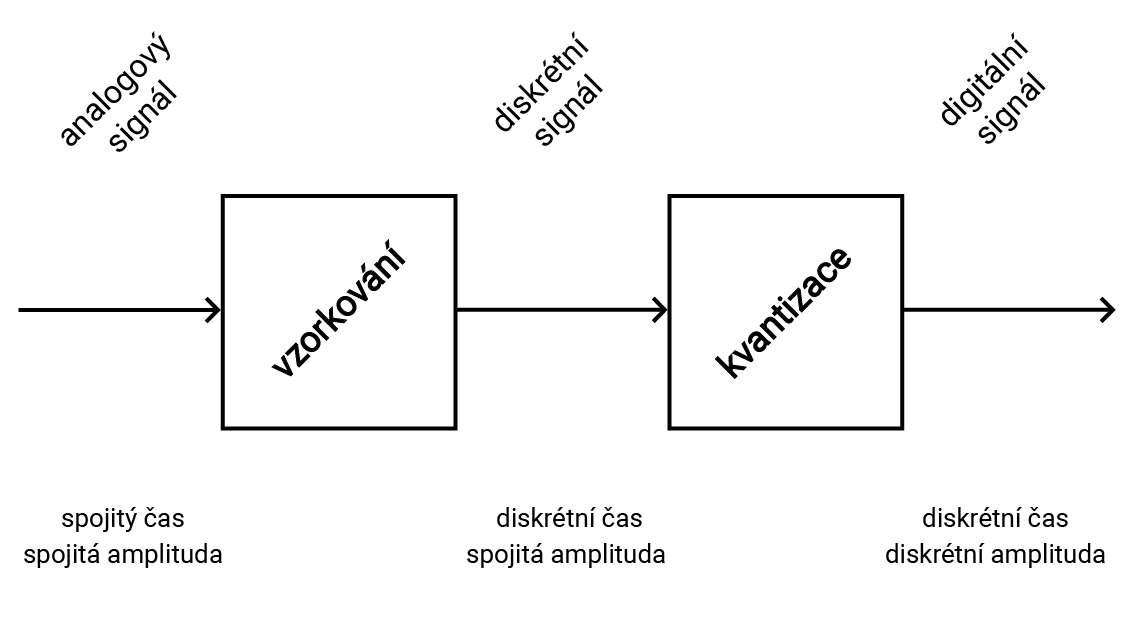
\includegraphics[width=340pt]{images/digitalizace.png}
%         \caption[]{\label{}Digitalizace zvuku.}
% \end{figure}



\pagebreak

%\begin{figure}[h]
 %   \centering
 %   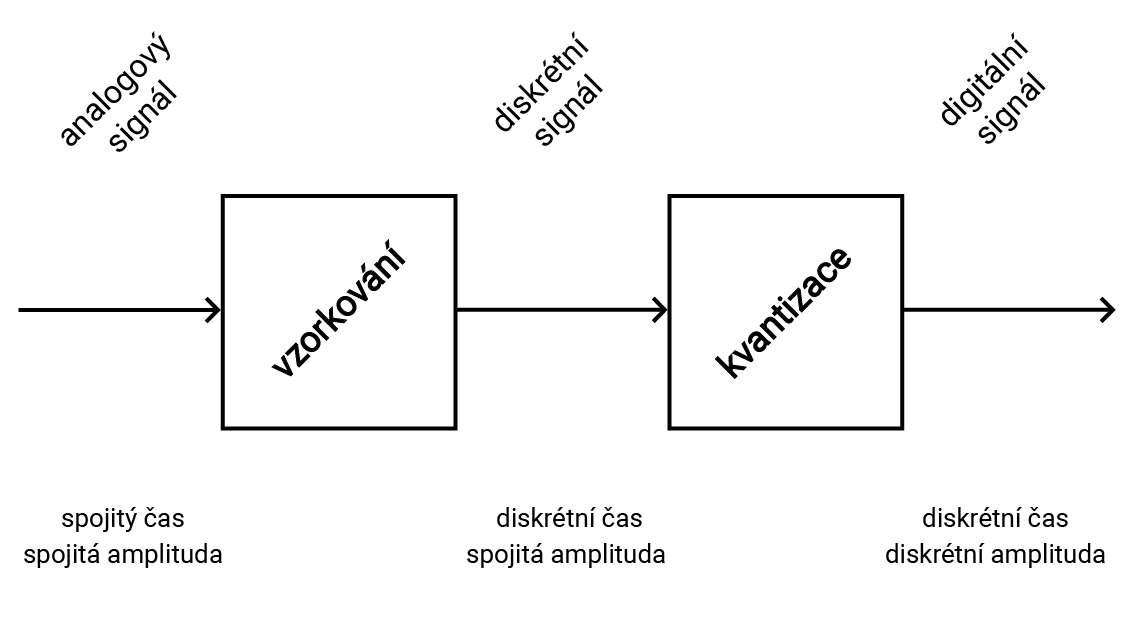
\includegraphics[width=340pt]{images/digitalizace.png}
  %      \caption[]{\label{}Digitalizace zvuku.}
%\end{figure}

\subsection*{Vzorkování}

Prvním krokem v digitalizaci zvuku je vzorkování, nebo-li diskretizace signálu v čase. Nižší vzorkovací frekvence způsobí, že nebude slyšet celé slyšitelné spektrum původní nahrávky, nebo budou vyšší frekvence již zkreslené. Jaká by měla být správně vzorkovací frekvence udává \textbf{Nyquistův–Shannonův vzorkovací teorém} \cite{nyquist}:
%\todo[fancyline]{ref az nekde jinam do textu} %\ref{eq:1}

\begin{equation} \label{eq:1}
    {\displaystyle f_{v}>2f_{\max }\left[s^{-1}\right]} \enspace .
\end{equation}

V doslovném znění: „Přesná rekonstrukce spojitého, frekvenčně omezeného signálu z jeho vzorků je možná tehdy, pokud byla vzorkovací frekvence vyšší než dvojnásobek nejvyšší harmonické složky vzorkovaného signálu.“ V případě použití nižší vzorkovací frekvence může dojít k tzv. aliasingu, kdy rekonstruovaný signál je výrazně odlišný od původního vzorkovaného signálu.

\subsection*{Kvantování}

Kvantování je diskretizace signálu v oboru hodnot, čili v amplitudě. Pokud kvantování není dostatečně jemné, vznikají falešné kvantizační hrany a tedy kvantizační šum.

\begin{figure}[h]
\def\svgwidth{0.8\textwidth}
  \captionsetup{justification=centering}
    \centering
    \input{images/dig.eps_tex}
        \caption[Digitalizace signálu.]{ 
        Schématické znázornění digitalizace zvuku s časem na ose \textit{x}. Zleva původní analogový signál s elektrickým napětím na ose\textit{ y}, uprostřed znázornění vzorkování signálu a vpravo kvantování, které bude následně reprezentováno bitově.}
        % https://www.ux1.eiu.edu/~cfadd/1150/16Waves/char.html
        % https://ux1.eiu.edu/~cfadd/3050/Adventures/chapter_12/ch12_3.htm
    \label{fig:digitalization}
\end{figure}

\section{Způsob zaznamenání zvuku}

Nynější digitální forma záznamu na audio soubor musela ujít dlouhou cestu. Namátkou například přes kamenné desky, notové zápisy, děrné pásky pianoly, gramofonové desky, magnetické pásky atd. Některé způsoby jako třeba notové zápisy stále mají svůj nenahraditelný význam. Záleží tudíž na výhodách, jaké konkrétní interpretace přinese a jak jich využít\footnote{Zvuk může být obsažen i v kvalitně pořízeném videu bez zvuku. Podle \cite{visual-microphone} lze zvuk z videa zpětnou rekonstrukcí získat, ovšem výsledná kvalita zvuku se samozřejmě nedá uvažovat jako optimální k účelům vizualizace hudby.}. 


\paragraph*{Audio soubor}

% \cite{Kabelka} 


reprezentace pro digitální použití nejtypičtější. Dle \cite{Kabelka4122018} má soubor daný formát a skládá se většinou ze tří částí: hlavičky, metadat a samotných zvukových dat. Hlavička identifikuje formát souboru a parametry zvukových dat (vzorkovací frekvence, bitová hloubka, počet kanálů). \emph{Metadata} obsahují informace o autorovi, v případě hudební stopy ještě např. název skladby, alba apod. {Zvuková data} reprezentují samotný zvukový záznam. Způsob ukládání zvukových dat je závislý na počtu kanálů zvuku. Vícekanálové audio, ať už stereo (dva kanály), nebo prostorové (5 kanálů), má většinou v souboru pro každý kanál vyhrazené příslušné místo. 

%\todo[fancyline, color=green]{jen vsuvka - standartni zvyrazneni je pomoci \emph{\\emph} - ktere dela v romro pripade (da se predefinovat) italiku. v zasade je ale jendo co a jak pouzijete, pokud se toho budete drzet (tedy klicova slova / terminy, odstavce, atd.).}

\paragraph{\gls{midi}}
%
% \todo[fancyline, color=green]{na drurazneni klicovych slov ktere nechcete ale v obsahu se taky da pouzivat paragraph (https://en.wikibooks.org/wiki/LaTeX/Paragraph\_Formatting)}
%
je rozhraní (standard) používané pro komunikaci elektronických hudebních nástrojů. \gls{midi} je digitálním popisem zvukového záznamu, tzn. souborem informací o výšce jednotlivých tónů, jejich intenzitě, délce, nejrůznějších efektech a jiných informací charakterizujících výsledný sluchový efekt zvukového záznamu. Tyto informace pak zpracovává výstupní zvukové zařízení, které je schopné vytvářet nejrůznější zvuky (zvuková karta či syntezátor).

% http://shellin.wz.cz/midi.php

Tento digitální popis zvukového záznamu je vhodný pro vizualizace. Otázkou jen zůstává, jak se takový záznam získá. Některá zařízení, jako jsou například \gls{midi} klávesy, poskytují snadný způsob získávání \gls{midi} not přímo z hrané hudby. V případě hudby získané bez speciálních zařízení (tradičních hudebních nástrojů, zpěvu, ...) může být pro \gls{midi} reprezentace provedena konverze pomocí specializovaných programů\footnote{Základní rozpoznávání tónů poskytuje i ladička na kytaru.}. Například software \textit{Dubler Studio Kit \cite{DublerStudioKit}} převádí v reálném čase zpěv na \gls{midi} reprezentaci.

% http://www.shellin.wz.cz/midi1.htm

\paragraph*{Stem}

je audio formát od německé firmy \textit{Native Instruments}. Jde o vícekanálový zvukový formát, který usnadňuje práci se zvukem. Obsahuje kromě standardní stereo stopy ještě další čtyři vrstvy audiosignálu. Jednotlivé vrstvy v praxi zastupují čtveřici zvukových „stop“, které dohromady tvoří kompletní skladbu – typicky například bicí-basa-synth-vokál a pomocí kompatibilních ovladačů je lze samostatně ovládat.

% http://www.muzikus.cz/pro-muzikanty-novinky/Native-Instruments-novy-audio-format-STEM~10~srpen~2015/



%\begin{figure}
% \centering
%  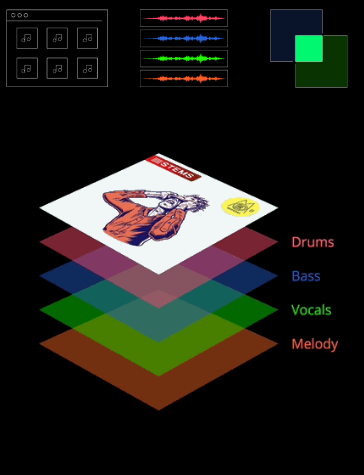
\includegraphics[width=290pt]{images/stem.png}
%  \caption{Znázornění obsahu STEM formátu}
%  \label{fig:stem}
%\end{figure}

% \section{Vlastnosti hudby}

%\begin{description}
%  \item [Dynamika]\hfill \\
%Průběh hlasitosti v čase.

%Na žánru je také závislý dynamický
%rozsah, což je rozdíl hlasitostí mezi nejtišším a nejhlasitejším bodem nahrávky
%  \item [Tempo] \hfill \\
%BPM


%\item [Vzorkovací frekvence, počet bitů] \hfill \\
%Vychází ze vzorkování a kvantování.

% http://www-labs.iro.umontreal.ca/~pift6080/H09/documents/papers/scheirer_jasa.pdf
%\end{description}

%\todo[fancyline,color=red]{nezapomente na klasicke 440 Hz, 880 Hz, 1320 Hz, 1760 Hz (ladeni)}

\newpage

\section{Vlastnosti hudebních signálů}
% https://is.muni.cz/th/blifg/dp.pdf

Existují subjektivní atributy, které jsou při charakterizaci hudebních signálů obzvláště užitečné. Jsou jimi: výška, síla (hlasitost) a témbr (barva)\footnote{Diplomová práce \cite{Holcik2009} popisuje vlastnosti hudebních signálů podrobněji.}.

\paragraph{Výška}

 je charakteristika, která umožňuje seřazení zvuků na frekvenční stupnici zespodu nahoru. Přesněji je výška definovaná jako frekvence sinusové křivky, která je přiřazena zdrojovému zvuku lidským posluchačem.

\paragraph{Hlasitost}

 se v počítačovém zpracování hudby se často udává v decibelech, logaritmické fyzikální jednotce, jelikož lidské tělo vnímá podněty logaritmicky jejich intenzitě.

\paragraph{Barva} \label{tebr}

 je vlastnost, díky které můžeme od sebe rozeznat např. zvuky houslí a flétny, které mohou být identické co do výšky, hlasitosti a délky. Koncept této vlastnosti se nedá jednoduše vyjádřit nějakou fyzikální vlastností zvuku, ale spíše souvisí s rozložením spektrální energie a její distribucí v čase jak je ukázáno na obrázku \ref{fig:tebr}.
 

%  "Zatímco výška, hlasitost a délka zvuku mohou být jednoduše zaznamenány skalární hodnotou, barva je vícerozměrný koncept a je typicky reprezentována vektorem charakteristik. S barvou zvuku velice úzce souvisí tzv. vyšší harmonické frekvence (alikvotní tóny), které nástroje generují."  \cite{Holcik2009} 


% \todo[fancyline]{pouzil bych citacni prostredi} => Cely text vychazi z prace Holcika, nejen tento jeden odstavec

% \begin{quote}[Spektrální analýza hudební skladby \cite{Holcik2009}]{Lukáš Holčík}
% \end{quote}
\begin{figure}[h]
\def\svgwidth{0.65\textwidth}
    \centering
    \input{images/timbre.eps_tex}
        \caption{Náčrt průběhu signálu noty C hrané na různé nástroje.}
        % https://www.ux1.eiu.edu/~cfadd/1150/16Waves/char.html
        % https://ux1.eiu.edu/~cfadd/3050/Adventures/chapter_12/ch12_3.htm
    \label{fig:tebr}
\end{figure}

 Zatímco výška, hlasitost a délka zvuku mohou být jednoduše zaznamenány skalární hodnotou, barva je vícerozměrný koncept a je typicky reprezentována vektorem charakteristik. S barvou zvuku velice úzce souvisí tzv. vyšší harmonické frekvence (alikvotní tóny), které nástroje generují.


\newpage

\section{Fourierova transformace} \label{fourier}


%\begin{figure}[]
  %\centering
  %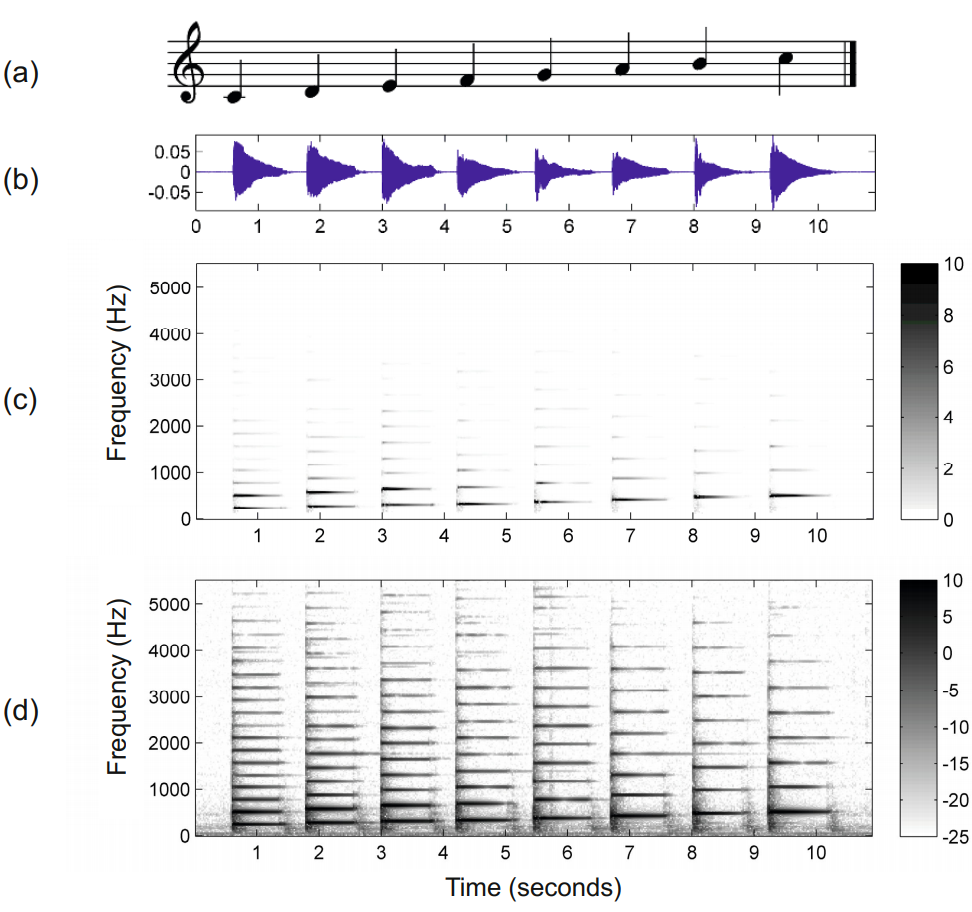
\includegraphics[width=385pt]{images/notes.png}
%  \caption{Waveform and spectrogram of a music recording of a C-major scale played on a piano.
%  (a) The recording’s underlying musical score. (b) Waveform. (c) Spectrogram. (d) Spectrogram
%  with the magnitudes given in dB. \cite{cmajor}}
%  \label{fig:cmajor}
%\end{figure}


\par
% http://boemers.de/personal/thesis.pdf !!!!!!!!!!!!!!!!!!!!!!!!!!!!!!!!
% https://is.muni.cz/th/blifg/dp.pdf


Fourierova transformace je ve vizualizaci hudby hojně využívaná. Za jejím vznikem stojí původně kontroverzní myšlenka Jeana Baptisty Josefa Fouriera (1768-1830), že spojitý periodický signál může být reprezentován součtem správně zvolených sinusových vln. Dnes víme, že tomu tak opravdu je (zvolených sinusových vln může být nekonečně mnoho).

Běžné signály jsou tvořeny směsí signálů o různých frekvencích. Postupy, které slouží k výpočtu frekvenčního spektra, jsou označovány jako \emph{Fourierova analýza}. Toto souhrnné označení se rozděluje do kategorií podle druhu signálu. Singál může být diskrétní, či spojitý a periodický, či neperiodický. 

Pro analýzu hudební nahrávky je vhodné použít \emph{diskrétní Fourierovu transformaci\footnote{Discrete Fourier Transform}} (DFT) pro periodicky opakující se signály definované na diskrétních bodech v čase. V praxi se používá \emph{rychlá Fourierova transformace\footnote{Fast Fourier Transform}} (FFT), jakožto efektivní algoritmus pro výpočet diskrétní Fourierovi transformace.

\begin{figure}[h]
\def\svgwidth{1\textwidth}
    \centering
    \input{images/fourier.eps_tex}
        \caption[Fourierova transformace.]{
        Znázornění Fourierovy transformace.}
    \label{fig:fourier}
\end{figure}

Pomocí Fourierovi transformace lze převést signál z reprezentace závislé na čase na reprezentaci závislé na frekvenci (což je schématicky znázorněno na obrázku \ref{fig:fourier}\footnote{Zdroj: \url{https://tech.liuchao.me/2018/05/polynomial-multiplication/}}). Na zpětnou transformaci lze použít inverzní Fourierovu transformaci. Fourierova transformace $S(\omega )$
funkce $s(t)$ je definována integrálním vztahem \ref{eq:2}, a to jako:
%S(\omega )}S(\omega )  {\displaystyle s(t)}s(t) je d



\begin{equation} \label{eq:2}
    S(\omega ) = \int_{-\infty}^{\infty}{s(t)e^{-i\omega t}dt}\enspace .
    % {\displaystyle f_{v}>2f_{\max }\left[s^{-1}\right]} 
\end{equation}





\newpage


% \begin{figure}[]
%    \centering
%    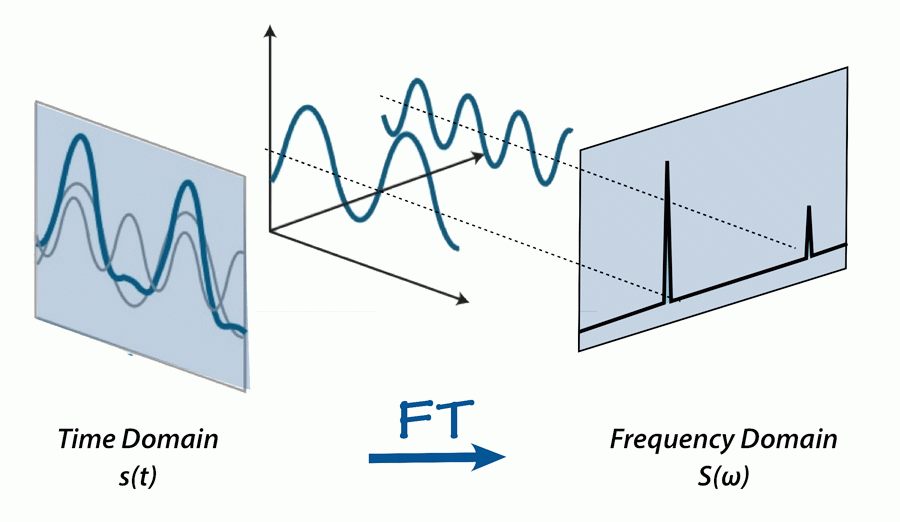
\includegraphics[width=300pt]{images/fourier.png}
%        \caption{Fourierova transformace}
%        \label{fig:fourier}
%\end{figure}

% \subsection*{Vlnková trasnformace}

% Efekt zvuků slyšitelný na různých frekvencí je zhruba následující:

% \begin{description}
%  \item [Sub-bass]        20 až 60 Hz \hfill \\
%  The sub bass provides the first usable low frequencies on most recordings. The deep bass produced in this range is usually felt more than it is heard, providing a sense of power. Many instruments struggle to enter this frequency range, with the exception of a few bass heavy instruments, such as the bass guitar which has a lowest achievable pitch of 41 Hz. It is difficult to hear any sound at low volume level around the sub bass range due to the Fletcher Munson curves (Equal Loudness Curves).
  %\item [Bass]            60 až 250 Hz \hfill \\
%  The bass range determines how fat or thin the sound is. The fundamental notes of rhythm are centered on this area. Most bass signals in modern music tracks lie around the 90-200 Hz area. The frequencies around 250 Hz can add a feeling of warmth to the bass without loss of definition.
%  \item [Low midrange]    250 až 500 Hz \hfill \\
%  The low midrange contains the low order harmonics of most instruments and is generally viewed as the bass presence range.
%  \item [Midrange]        500 Hz až 2 kHz \hfill \\
  %The midrange determines how prominent an instrument is in the mix. Boosting around 1000 Hz can give instruments a horn like quality. Excess output at this range can sound tinny and may cause ear fatigue. If boosting in this area, be very cautious, especially on vocals. The ear is particularly sensitive to how the human voice sounds and its frequency coverage.
 % \item [Upper midrange]  2 až 4 kHz \hfill \\
 % Human hearing is extremely sensitive at the high midrange frequencies, with the slightest boost around here resulting in a huge change in the sound timbre. The high midrange is responsible for the attack on percussive and rhythm instruments. If boosted, this range can add presence. However, too much boost around the 3 kHz range can cause listening fatigue.
 % \item [Presence]        4 až 6 kHz \hfill \\
  %The presence range is responsible for clarity and definition of a sound. It is the range at which most home stereos center their treble control on.
 % \item [Brilliance]      6 až 20 kHz \hfill \\
  %The brilliance range is composed entirely of harmonics and is responsible for sparkle and air of a sound.
%\end{description}


%%%%%%%%%%%%%%%%%%%%%%%%%%%%%%%%%%%%%%%%%%%%%%%%%% POZNAMKY Z TEXTU:
%\section{Analysis and Visualisation of Music}
%\section{Music Visualization Based on Spherical Projection With Adjustable Metrics}
%\section{Isochords}

% \section{Detekce rytmu}

% Problematika detekce rytmu a určení BPM je důležitá například pro světelné efekty, DJ, úpravu audia, ale i doporučování hudby hudebními aplikacemi například na sport.

% https://en.wikipedia.org/wiki/Beat_detection
% https://www.eecs.qmul.ac.uk/~markp/2011/RobertsonStarkPlumbleyICMC2011_accepted.pdf
%https://www.teachmeaudio.com/mixing/techniques/audio-spectrum/
\section{Music Information Retrieval} \label{MIR}

\gls{mir} je zatím malý, ale rostoucí výzkumný obor s mnoho využitími. Je možné zde využít znalosti z muzikologie, psychoakustiky, psychologie, akademické hudební teorie, zpracování signálu, informatiky, strojového učení, optického rozpoznávání hudby, computational intelligence a kombinace těchto oborů. Mezi typické problémy řešené v oboru \gls{mir} patří:

\begin{itemize}
    \item systémy doporučování hudby,
    \item oddělování stop ze skladby a rozpoznávání nástrojů,
    \item automatický přepis hudby,
    \item automatická kategorizace,
    \item generování hudby.
\end{itemize}

\begin{figure}[h]
\centering
  \begin{subfigure}[b]{0.4\textwidth}
    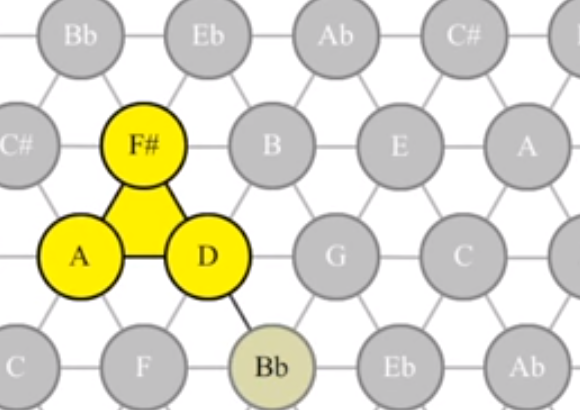
\includegraphics[width=\textwidth]{images/isochords.png}
    \caption{Tonnetz diagram}
  % https://www.youtube.com/watch?v=NQ7LkWCzKxI
    \label{fig:tonnetz}
  \end{subfigure}
  %
  \begin{subfigure}[b]{0.4\textwidth}
    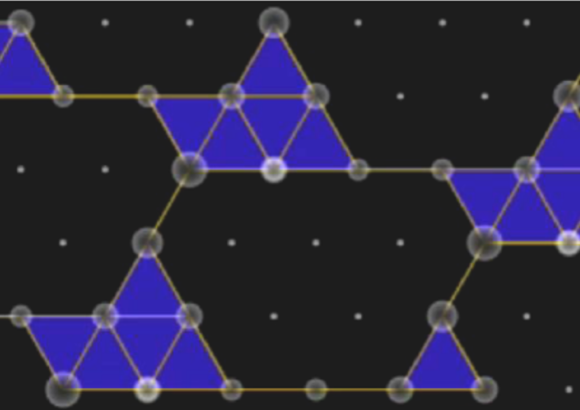
\includegraphics[width=\textwidth]{images/isochords2.png}
    \caption{Isochords}
    \label{fig:iso}
  \end{subfigure}
    \label{fig:isochords}
    \caption{Isochords a Tonnetz diagram.}
\end{figure}

\subsection*{Isochords - vizualizace struktury v hudbě}
Je mnoho prací, týkajících se tématiky MIR. Jednou z nich je práce \cite{isochords} z roku 2007 představující \textit{Isochords}. Jde o vizualizaci, která pomáhá při klasifikaci hudebních struktur.
Předává informace o kvalitě intervalu, kvalitě akordu a průběhu akordu při přehrávání digitální hudby. Nabízí posluchači způsob uchopení základní struktury hudby bez nutnosti rozsáhlého tréninku. Pro vizualizaci používá Tonnetz\footnote{Tonnetz (německy zvuková síť) reprezentuje tonální prostor, který poprvé popsal Leonhard Euler roku 1739.} - konceptuální mřížkový diagram. Na obrázku \ref{fig:tonnetz}\footnote{Zdroj: \url{youtu.be/NQ7LkWCzKxI}} je ukázka Tonnetz diagramu a na \ref{fig:iso} Isochords představené v práci \cite{isochords}.

\pagebreak

\begin{figure}[t]
  \centering
  \captionsetup{justification=centering}
  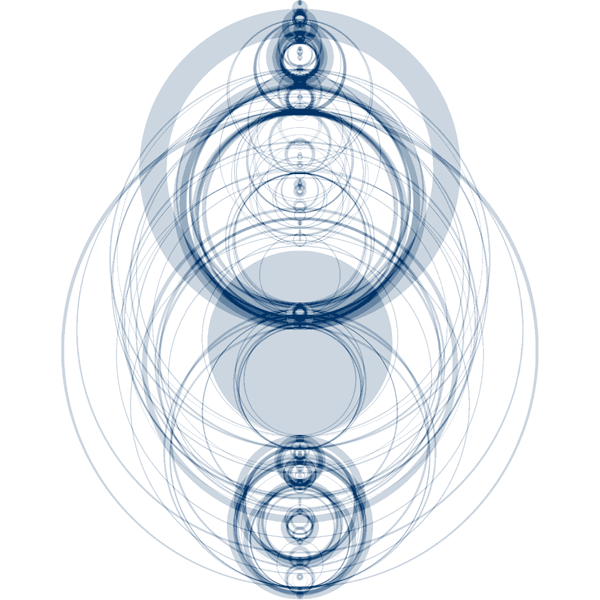
\includegraphics[width=360pt]{images/vivaldi.png}
  \caption[Arc diagram.]{\textit{Arc diagram} vizualizující Vivaldiho Podzim ze Čtvera ročních období}
  % http://www.bewitched.com/song.html
  \label{fig:vivaldi}
\end{figure}

\subsection*{Vizualizace sémantických struktur v klasické hudbě}
Wingova práce \cite{Wing} z roku 2009 je jedno z mnoha prací navrhující zajímavý způsob, jak vizualizovat klasickou hudbu. Obsahuje objemnou rešerši, ve které kromě \textit{Isochords} a mnohých dalších projektů a možností vizualizace hudby autor zmiňuje tzv. \textit{arc diagram}\footnote{Obloukový diagram}.

\textit{Arc diagram} lze použít na zobrazení opakujících se struktur spojením stejných podřetězců polokruhem. Na obrázku \ref{fig:vivaldi}\footnote{Zdroj: \url{http://www.bewitched.com/song.html}} je znázorněna klasická skladba Podzim od Antonia Vivaldiho (s použitím kruhů místo polokruhů).



\newpage

\subsection*{Současný postup získávání informací z hudebních dat} \label{chroma}


Lopez-Rinconova práce \cite{Rincon} z roku 2019 rovněž diskutuje existující možnosti vizualizace hudby (jakými jsou například \textit{ImproViz} a \textit{MIDIVis}) a navrhuje vlastní způsob, na jehož počátku je \gls{midi} soubor. 

Postupnými kroky je obdržen 12-rozměrný vektor, jehož dimenze postupně reprezentují noty chromatické stupnice\footnote{Stupnice, rozdělující oktávu, interval mezi dvěma tóny, jejichž poměr frekvencí je 2:1, na dvanáct stupňů, mezi nimiž je vzdálenost jeden půltón.}: \textit{[C, C\sh, D, D\sh, E, F, F\sh, G, G\sh, A, A\sh, B]}. Hodnoty vektoru jsou binární a v případě, že je nota v daný čas přítomna, je na její pozici hodnota 1. Například pokud je sekvence not \textit{C, E, G} vypadají hodnoty vektoru následovně: \textit{[1, 0, 0, 0, 1, 0, 0, 1, 0, 0, 0, 0]}. Výsledné hodnoty jsou v práci mapovány pomocí sférické projekce.

Poptávka po algoritmech tohoto typu je především ze stran velkých společností pro streamovanou\footnote{Streamování je technologie kontinuálního přenosu audiovizuálního materiálu mezi zdrojem a koncovým uživatelem.} hudbu jako jsou \textit{Spotify}, \textit{Deezer}, \textit{Apple Music}, \textit{Google Play Music} a další. Některé společnosti jako je \textit{Spotify} umožňují vývojářům používat své nástroje pro analýzu, nebo alespoň výstupy z analýzy zkrze \gls{api}, zpřístupněného pro veřejnost.


% Následují novější práce z roku 2019. Práce \cite{Rincon} od autorů O. Lopez-Rincon a O. Starostenko navrhuje způsob, jak normalizovat data v MIDI souborech pomocí 12 dimenzionálního vektoru popisující získanou tonalitu, techniku redukce dimenzí a vizualizace získaných hudebních dat 3D projekcí.

% \subsection*{Analýza a vizualizace hudby}

% Práce \cite{Taenzer} analyzuje a vizualizuje hudbu pomocí jednoduchých světel pohybujících se podle výšky melodie hrané nástroji, nebo vokálů. Z toho důvodu byly zkoumány možnosti oddělení zdrojů zvuku a \textit{pitch detektor} pro odhad základních frekvencí.

% \subsection*{Vizualizace hudebních kolekcí}

%  Vizualizovat lze i hudební kolekce, jak bylo ukázáno v krátké práci \cite{Langer2008}.

\subsection*{Organizace a události}

Vyhodnocování výsledků v oblasti \gls{mir} a dalšímu zkoumání tohoto oboru se věnuje hned několik organizací, pracovišť a jednotlivců, například organizace ISMIR\footnote{International Society for Music Information Retrieval} a událost MIREX\footnote{Music Information Retrieval Evaluation eXchange}: 

\begin{description}
    \item [ISMIR] je nezisková organizace, mimo jiného dohlížející na organizaci \textit{\mbox{ISMIR}} konference. Tato každoroční konference je předním světovým fórem ve zpracování, hledání, organizování a přístupu k datům souvisejícím s hudbou.
    \item [MIREX] je každoroční vyhodnocování MIR algoritmů, spojené s \textit{ISMIR} konferencí. Je to soubor komunitně definovaných formálních hodnocení, prostřednictvím kterých je vyhodnocována široká škála nejmodernějších systémů, algoritmů a technik za kontrolovaných podmínek.
\end{description}

% \todo[color=green]{prosel jsem to a beru kapitolu jako kompletni}
% http://www.mmi.ifi.lmu.de/lehre/ws0809/hs/docs/langer.pdf



\chapter{Nástroje pro hudební analýzu}

V této kapitole lze nalézt několik vybraných nekomerčních programů, knihoven a \gls{api} pro analýzu hudby. Často v nějaké podobě využívají Fourierovu transformaci stručně popsanou v sekci \ref{fourier} předchozí kapitoly. 

% \todo[color=green]{prosel jsem to a beru kapitolu jako kompletni}

\section{Sonic visualiser}

Sonic Visualiser \cite{SonicVisualiser} je aplikace pro zobrazování a analyzování hudebních souborů. Je dostupný zadarmo pro Linux, OS X i Windows a distribuovaný pod GNU licencí. V základu nabízí různé možnosti vizualizace skladby:
\begin{description}
    \item [waveform] - průběh signálu; vzhled grafu zachycujího závislost okamžité hodnoty signálu na čase,
    \item [spectrogram] - vizuální reprezentace spektra frekvencí,
    \item [melodic range spectrogram] - spektrogram melodického rozsahu,
    \item [peak frequency spectrogram] - spektrogram nejvyšších frekvencí,
    \item [spectrum] - amplitudy frekvencí v daném čase.
\end{description}
%\newpage

Výhodou je sbírka specializovaných \emph{pluginů}\footnote{Plugin je doplňkový modul aplikace rozšiřující její funkčnost.} třetích stran, vhodných pro výzkumnou analýzu i pro hudebníky. Na obrázku \ref{fig:sonic} je vizualizováno prvních 5 vteřin skladby Hurt od Johnyho Cashe a použití pluginu \textit{Chordino} k odhadu akordů.


\begin{figure}[h]
  \centering
  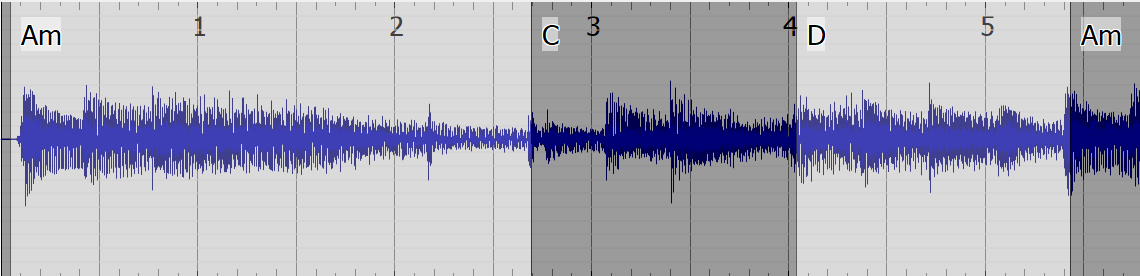
\includegraphics[width=360pt]{images/cash_chords.png}
  \caption{Program \textit{Sonic Visualiser} a plugin \textit{Chordino} pro odhad akordů}
  \label{fig:sonic}
\end{figure}


% https://code.soundsoftware.ac.uk/projects/sonic-visualiser
% https://sonicvisualiser.org/sv2010.pdf

% https://www.youtube.com/watch?v=IRrUdywsrNU
% https://github.com/willianjusten/awesome-audio-visualization


\section{Spleeter}

Běžná audio nahrávka má všechny nástroje a vokály neoddělitelně spojeny a je proto těžké manipulovat například pouze se zvukem klavíru. Francouzská online streamovací služba \textit{Deezer} představila svoji open-source knihovnu, která dokáže audio rozložit na několik částí. State-of-the-art\footnote{Obecně nejmodernější, nejvyšší stupeň vývoje v oboru.} knihovna Spleeter\cite{spleeter2019} je napsána v programovacím jazyce Python a používá platformu pro strojové učení TensorFlow. Poskytuje natrénovaný model pro separaci audia na následující části:

\begin{itemize}
  \item vokály / doprovod (2 stems)
  \item vokály / bicí / basy / ostatní (4 stems)
  \item vokály / bicí / basy / klavír / ostatní (5 stems)
\end{itemize}

Rozdělení audia pomocí Spleeteru lze bez nutnosti instalování knihoven na různých webových stránkách, či lokálně na svém počítači. V dokumentaci programu Spleeter \cite{spleeterDoc} je například uvedeno, že při spuštění na GPU lze oddělit zvukové soubory na 4 stems 100 krát rychleji, než v reálném čase.


\section{WaoN}

WaoN (neboli Wave-to-Notes) je program, který napsal Kengo Ichiki. Slouží jako Unixový nástroj pro převod zvuku do not. Kód je dostupný pod licencí \textit{GNU General Public License v2.0}. Je složen ze tří programů:
\begin{description}
    \item [waon] -- konvertor z WAV do \gls{midi} formátu 
    \item [pv] -- fázový vokodér\footnote{Z anglického \textit{voice encoder}; slouží k syntéze zvuku a řeči} pro \textit{time-streching}, neboli proces pro změnu rychlosti či trvání audio signálu za zachování stejné výšky (\textit{pitch}) a \textit{pitch-shifting}, neboli transpozice
    \item [gwaon] -- \gls{gui} pro programy \textit{WaoN} a \textit{pv}
\end{description}


\begin{figure}[t]
\def\svgwidth{0.9\textwidth}
    \centering
  \captionsetup{justification=centering}
    \input{images/spotify_export.eps_tex}
        \caption[Znázornění \textit{Spotify API} intervalů ve skladbě.]{
        Dvacet sekund skladby "Around the World" od Daft Punk a vizualizace odhadovaných událostí v hudbě.}
        % https://www.ux1.eiu.edu/~cfadd/1150/16Waves/char.html
        % https://ux1.eiu.edu/~cfadd/3050/Adventures/chapter_12/ch12_3.htm
    \label{fig:spotify}
\end{figure}


\section{Spotify API}
\label{spotify}

\textit{Spotify} je jedna z mnoha služeb, nabízející streamovanou hudbu a podcasty. Uživatelé mohou kromě přehrávání zvukových záznamů například vytvářet veřejné, soukromé a sdílené playlisty.

\textit{The Echo Nest}, platforma, kterou od roku 2014 vlastní \textit{Spotify}, se specializuje na vývoj v oblasti hudby, umožňuje vytvářet algoritmická hudební doporučení, a tím tak předpovídat, jaká skladba se uživateli bude líbit. 
% https://developer.spotify.com/community/news/2014/06/17/say-hello-new-web-api/

%Uživatel může ovládat službu z jiného zařízení, než na kterém je přihlášen, což v kombinaci se Spotify \gls{api} dostupným pro veřejnost otevírá možnosti pro integrování \textit{Spotify} do vlastních aplikací.





% Po červnu 2014 příchod Web API umožnil vývojářům třetích stran integrovat Spotify obsah do jejich vlastních aplikací. Používá REST principy a ovládání pomocí HTTP požadavků, která vracejí data ve formátu JSON. Možnsoti Spotify API jsou následující:

% https://developer.spotify.com/documentation/web-api/reference-beta/#endpoint-get-audio-analysis

% \subsection*{Spotify \gls{api}}

% \gls{api} specifikuje způsob, jakým jsou data přenášena mezi platformami. Spotify \gls{api} využívá styl architektury REST\footnote{Representational State Transfer} používající pro výměnu dat HTTP\footnote{Hypertext Transfer Protocol} požadavky. Kromě očekávaných \textit{endpointů}\footnote{Endpointem je myšlena adresa pro posílání HTTP požadavků.} pro přihlašování a přehrávání hudby umožňuje vývojářům přistupovat k \textit{endpointům} pro analýzu skladby a informace o skladbě. Spotify \gls{api} tudíž umožňuje nejen vytvořit vlastní plnohodnotný přehrávač, ale disponuje nástroji pro hudební analýzu a tedy i vizualizace.
% https://developer.spotify.com/community/showcase/

\subsubsection*{Analýza skladby (Get Audio Analysis)}
% Get a detailed audio analysis for a single track identified by its unique Spotify ID.
% http://docs.echonest.com.s3-website-us-east-1.amazonaws.com/_static/AnalyzeDocumentation.pdf

Některé ze \textit{Spotify} \gls{api} \textit{endpointů} jsou vhodné k vizualizaci skladeb. Analýza skladby mezi ně patří, jelikož poskytuje odhadované události v konkrétní skladbě. Skladbu dělí na \textit{bars} (takty), \textit{beats} (doby), \textit{sections} (sekce), \textit{segments} (segmenty) a \textit{tatums} (tatumy). Význam rozdělení je popsán v tabulce \ref{table:sections} a graficky zakreslen v obrázku \ref{fig:spotify}.




%For completeness however, the first dimension represents the average loudness of the segment; second emphasizes brightness; third is more closely correlated to the flatness of a sound; fourth to sounds with a stronger attack; etc

% \begin{figure}[h]
%   \centering
%   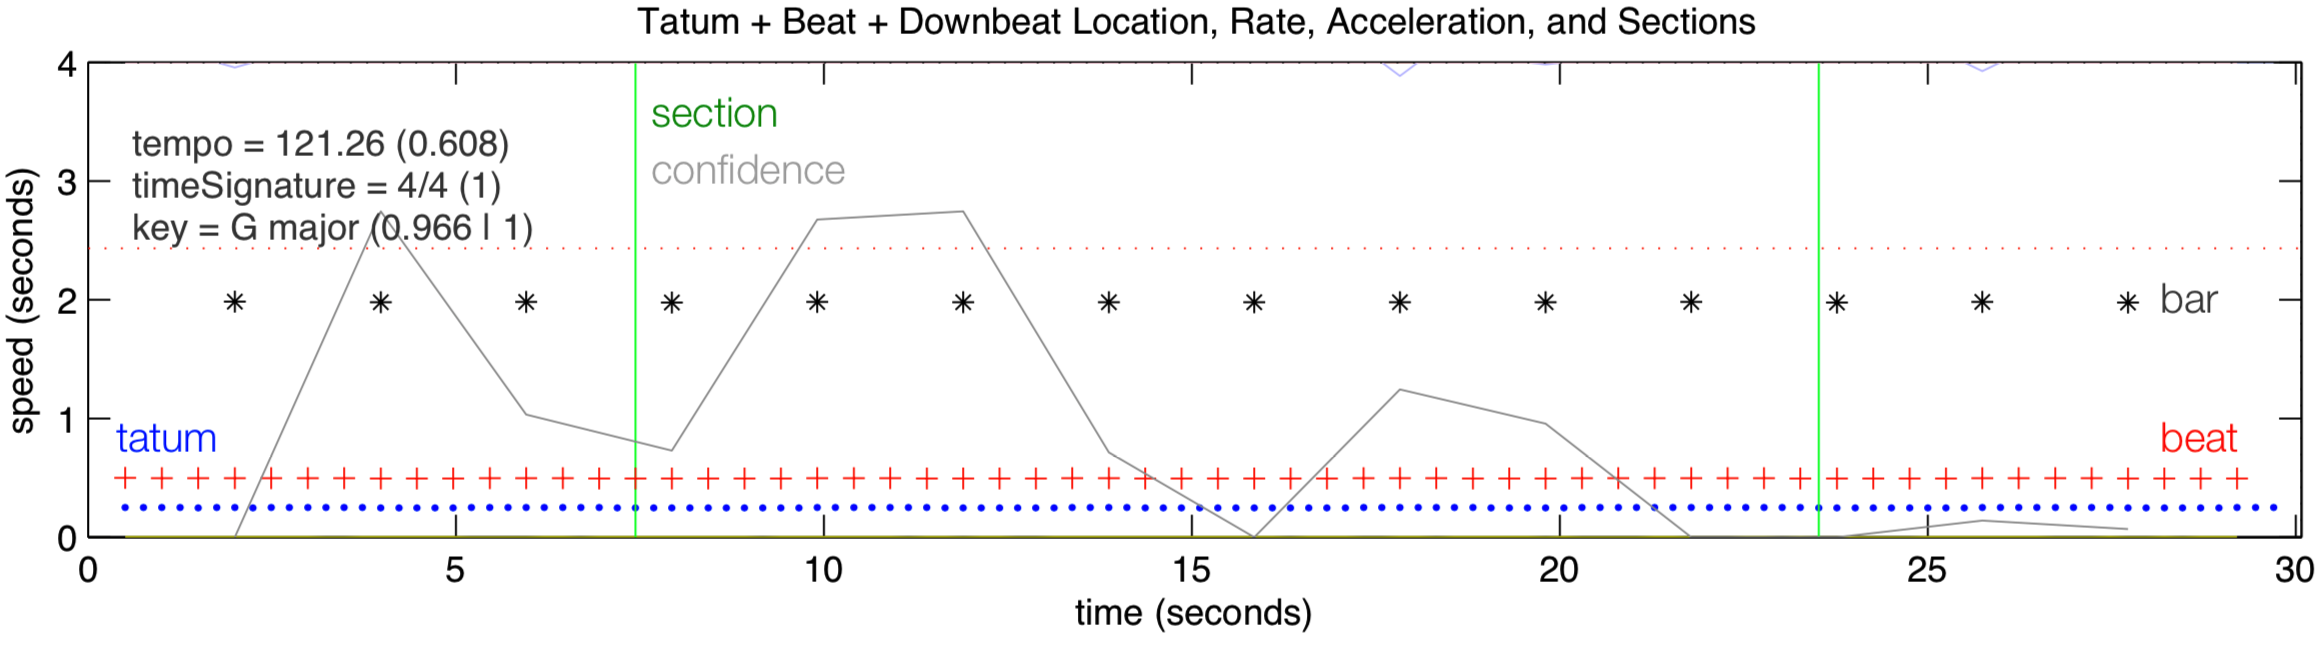
\includegraphics[width=370pt]{images/Rhythm.png}
%   \centering
%   \caption{Třicet sekund skladby "Around the World" od Daft Punk a vizualizace odhadovaných událostí v hudbě}
%   \label{fig:spotify}
% \end{figure}

% \vspace{6mm}

\begin{table}[]
\begin{tabular}{@{}ll@{}}
\toprule
Dělení skladby   & Popis objektů rozdělující skladbu \\ \midrule
Sekce & \begin{tabular}[c]{@{}l@{}}Nejdelší rozlišení skladby. Sekcí bývá označena například\\sloka, verš, kytarové sólo a tak dále.\end{tabular}  \\
Takty     & \begin{tabular}[c]{@{}l@{}}Označuje začátek taktu,  skládá se z několika dob.\end{tabular}                                                 \\
Doby    & \begin{tabular}[c]{@{}l@{}}Beat, neboli česky doba, je základní časová jednotka hudby. \\ Například tik metronomu.\end{tabular}                   \\
Segmenty & \begin{tabular}[c]{@{}l@{}}Segmenty, do kterých je skladba rozdělena, obsahují \\ zhruba konzistentní zvuk po dobu svého trvání.\end{tabular} \\
Tatumy   & \begin{tabular}[c]{@{}l@{}}Tatum reprezentuje nejnižší intuitivně slyšitelný\\pravidelný puls.\end{tabular}                                \\ \bottomrule
\end{tabular}
\caption{\label{table:sections}Význam objektů získaných z analýzy skladby přes \textit{Spotify} \gls{api}.}
\end{table}

% \begin{table}[b]
%   \captionsetup{justification=centering}
% \begin{tabular}{ 
% |p{\dimexpr.15\linewidth-2\tabcolsep-1.3333\arrayrulewidth}% column 1
% |p{\dimexpr.85\linewidth-2\tabcolsep-1.3333\arrayrulewidth}% column 2
% |}
% \hline
%     sections &   Nejdelší rozlišení skladby. Sekcí bývá označena například sloka, verš, kytarové sólo a tak dále. \\
% \hline
%     bars    &	Označuje začátek taktu. A skládá se z několika dob. \\
% \hline
%     beats   &	Beat, či česky doba je základní časová jednotka hudby. Například tik metronomu.  \\
% \hline
%     segments  &	Segmenty, do kterých je skladba rozdělena obsahují zhruba konzistentní zvuk po dobu svého trvání. \\
% \hline
%     tatums    &	Tatum reprezentuje nejnižší intuitivně slyšitelný pravidelný puls. \\
% \hline
% \end{tabular}
% \caption{\label{table:sections}Význam objektů získaných z analýzy skladby přes \textit{Spotify} \gls{api}.}
% \end{table}



\newpage



% https://github.com/spotify/web-api/issues/920
% https://github.com/spotify/web-api/issues/947

Skladba je rozdělena na překrývající se úseky (viz. \tablename~\ref{table:sections}) od nejdéle trvajících úseků po ty nejkratší. \textbf{Sekce}, \textbf{takty}, \textbf{doby}, \textbf{segmenty} a \textbf{tatumy} mají všechny atributy \textit{start} (začátek konkrétního objektu), \textit{duration} (dobu trvání) a \textit{confidence} (jistotu správného označení). 

\paragraph*{Sekce}

sekce v sobě obsahuje navíc atribut celkové hlasitosti v decibelech vhodný pro porovnávání relativní hlasitosti sekcí. Další atributy jako tonalita (mollová či durová), tempo, tónina a taktové předznamenání obsahují každý po jednom dalším atributu \textit{confidence} udávající jistotu odhadu.

% \begin{itemize}
%     \item loudness
%     \item tempo
%     \item tempo confidence
%     \item key
%     \item key confidence
%     \item mode
%     \item mode confidence
%     \item time signature
%     \item time signature confidence
% \end{itemize}

\paragraph*{Segment}

obsahuje navíc atributy podrobněji definující hlasitost segmentu (počáteční, nejvyšší a koncovou hlasitost segmentu v decibelech a čas ve kterém hlasitost segmentu dosáhne maxima) a přidává chromatický vektor určující \textit{pitch} podobný vektoru zmíněném v kapitole \ref{chroma} o \gls{mir}.

Barva (témbr) segmentu je určena ze spektrogramů a má tedy vysokou úroveň abstrakce. Je získána jako 12-dimenzionální vektor a pro správnou interpretaci je vyžedována znalost či intuice ve čtení spektrogramů. Dokumentace popisuje první dimenzi jako reprezentující průměrnou hlasitost segmentu, druhá dimenze vyjadřuje "jas", třetí nejvíce koreluje s "plochostí" \ zvuku, čtvrtá zvuky se silnějším "attackem". Na obrázku \ref{fig:timbre_spotify} je vektor a jeho dimenze. Vodorovná osa udává čas, svislá osa frekvenci a vynesena je pak amplituda v daném čase a frekvenci.
%\footnote{Zdroj: https://developer.spotify.com/documentation/web-api/reference/tracks/get-audio-analysis/}



% \begin{quote}[Objasnění dimenzí vektoru popisujícího barvu.]{Spotify dokumentace}
% % ZDROJ   : https://developer.spotify.com/documentation/web-api/reference/tracks/get-audio-analysis/
%  the first dimension represents the average loudness of the segment; second emphasizes brightness; third is more closely correlated to the flatness of a sound; fourth to sounds with a stronger attack; 
% \end{quote}

% \begin{quote}[Dodatečné informace (odpověď na platformě \textit{github})]{Mark Koh}
% % ZDROJ:     https://github.com/spotify/web-api/issues/947
% These basis functions were generated using a PCA\footnote{Principal Component Analysis} over the segment's spectrogram. The description of the first four dimensions is simply a human interpretation of the basis functions. While interpreting the other dimensions requires knowledge/intuition of spectrograms, you can get a sense of what each basis function evaluates by trying to imagine what the sound of the spectrogram representation would be.
% \end{quote}

\begin{figure}[h]
  \captionsetup{justification=centering}
  \centering
  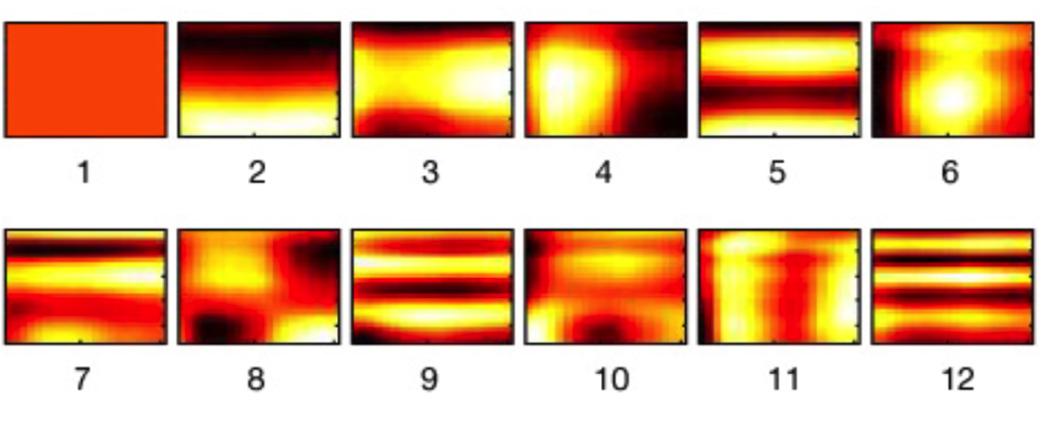
\includegraphics[width=280pt]{images/Timbre_basis_functions.png}
  \caption[Dvanáct bazických funkcí vektoru reprezentující barvu segmentu.]{Dvanáct bazických funkcí vektoru reprezentující barvu segmentu.}
  \label{fig:timbre_spotify}
\end{figure}


% \subsubsection*{Vlastnosti skladby (Get Audio Features)}

% Ke každé skladbě je možné získat dobu trvání, tóninu, tonalitu a taktové předznamenání\footnote{Připomenutí: vše kromě doby trvání je pouze odhad. Přesné algoritmy, které Spotify používá nejsou známy, ale lze se domnívat, že jde o podobné postupy, jako jsou použity v práci \cite{Rincon}.}. Mezi další atributy patří ty, popsané v tabulce \ref{table:features}\footnote{Dané termíny v tabulce \ref{table:features} se nepřekládají, aby se předešlo vzniku podivných neologismů. Místo toho je uveden jejich význam.}.  Ukázka průběhu zde pak demonstruje \figurename~\ref{fig:danceability}. Grafy k dalším atributům viz Přílohy. 

%Další informace např. o vztahu daných atributů a jejich rozsahu viz grafy ke každému atributu (Přilohy).

% \todo[fancyline]{j \imagee fajn priznavat ze je to spotify odhad, ale alespon bych napsal odhad na zaklade... nebo expertni odhad atp. }


% Get audio feature information for a single track identified by its unique Spotify ID.


% \begin{table}
% \begin{tabular}{ 
% |p{\dimexpr.25\linewidth-2\tabcolsep-1.3333\arrayrulewidth}% column 1
% |p{\dimexpr.75\linewidth-2\tabcolsep-1.3333\arrayrulewidth}% column 2
% |}
% \hline
%     acousticness    &	Pravděpodobnostní odhad akustičnosti skladby. Spotify API dokáže celkem sebejistě odadnout skladby, které akutické nejsou. \\
% \hline
%     danceability    &	Odhad jak moc je skladba vhodná k tanci v závislosti na kombinaci ukazatelů jako je tempo, stabilita rytmu, síla, and celková pravidelnost. \\
% \hline
%     energy  &	Energetické skladby působí rychle, hlasitě a hlučně. Mezi vjemové rysy přispívající k tomuto atributu patří dynamický rozsah, vnímaná hlasitost, zabarvení a rychlost nástupu.\\
% \hline
%     instrumentalness    &	Atribut dává pravděpodobností předpověď, jestli skladba je bez vokálů. Když je hodnota hodně blízko 1.0, patrně jde o skladbu beze slov. \\
% \hline
%     liveness    &	Snaha o rozhodnutí přítomnosti publika v nahrávce.  \\
% \hline
%     loudness    &	Hladina intenzity zvuku v decibelech (dB). Užitečné pro porovnání relativní hlasitosti stop.\\
% \hline
%     speechiness     &	Detekuje přítomnost mluveného slova. \\
% \hline
%     valence     &	Vysoká valence znamená pozitivní (šťastné, radostné, euforické) skladby, nízká negativní (smutné, depresivní, rozhněvané). \\
% \hline
%     tempo   &	Odhadované celkové tempo v BPM (beats per minute). \\
% \hline
% \end{tabular}
% \caption{\label{table:features}Tabulka odhadovaných vlastností skladby.}
% \end{table}

\begin{table}[]

\begin{tabular}{@{}ll@{}}
\toprule
Zkoumaná doména   & Popis upřesňující zkoumanou doménu  \\ \midrule
Acousticness    & \begin{tabular}[c]{@{}l@{}}
Pravděpodobnostní odhad akustičnosti skladby.  \end{tabular}  \\
Danceability & \begin{tabular}[c]{@{}l@{}}
Odhad jak moc je skladba vhodná k tanci v závislosti\\
na kombinaci ukazatelů jako je tempo, stabilita rytmu,\\
síla, a celková pravidelnost. \end{tabular}  \\
Energy          & \begin{tabular}[c]{@{}l@{}}
Mezi vjemové rysy přispívající k tomuto atributu\\
patří dynamický rozsah, vnímaná hlasitost, zabarvení\\
a rychlost nástupu. Energetické skladby působí rychle, \\ 
hlasitě a hlučně.\\ \end{tabular}  \\
Instrumentalness &   \begin{tabular}[c]{@{}l@{}}
Atribut udává pravděpodobností předpověď, jestli\\
skladba je bez vokálů. Když je hodnota hodně\\
blízko 1.0, patrně jde o skladbu beze slov. \end{tabular}  \\
Liveness          & \begin{tabular}[c]{@{}l@{}}
Pravděpodobnost přítomnosti publika v nahrávce. \end{tabular}  \\
Loudness & \begin{tabular}[c]{@{}l@{}}
Hladina intenzity zvuku v decibelech (dB). Užitečné\\
 pro porovnání relativní hlasitosti stop. \end{tabular}  \\
Speechiness  & \begin{tabular}[c]{@{}l@{}}
Odhad přítomnosti mluveného slova (např. recitativ). \end{tabular}  \\
Valence           & \begin{tabular}[c]{@{}l@{}}
Vysoká valence znamená pozitivní (šťastné, radostné,\\
euforické) skladby, nízká negativní (smutné, depresivní,\\
rozhněvané). \end{tabular}  \\
Tempo             & \begin{tabular}[c]{@{}l@{}}
Odhadované celkové tempo v BPM (beats per minute). \end{tabular}  \\ \bottomrule
\end{tabular}
\caption{\label{table:features}Tabulka odhadovaných vlastností skladby.}
\end{table}


%\todo[fancyline]{AAAaaa, podle me by se sem hodila stridava barva radku, ale nedari se mi ji sem dat.}
%\todo[fancyline, color=green]{ono se to moc nedela, byt to jde. - cellcolor plus opravene balicky u xcolor, pripadne proste color }
%\todo[fancyline]{Taky bych pridala preklad pod veci nalevo, ale nelibi se mi stylizace zalamovani}
%\todo[fancyline, color=green]{verim ze to tu hezkou tabulku asi rozbije... zatim bych neresil - resp. by to pak chtelo treba stejne dlouhe preklady (na radky) }

 \begin{figure}[h]
 \def\svgwidth{0.8\textwidth}
     \centering
     \input{images/danceability.eps_tex}
         \caption{Rozdělení hodnot funkce pro atribut \textit{danceability}.}
     \label{fig:danceability}
 \end{figure}

% \begin{figure}[b]
% \def\svgwidth{0.75\textwidth}
%     \centering
%     \input{images/acousticness.eps_tex}
%         \caption[]{
%         Distribuce hodnot atributu \textit{accousticness}.}
%     \label{fig:accousticness}
% \end{figure}

% \begin{figure}[b]
% \def\svgwidth{0.75\textwidth}
%     \centering
%     \input{images/danceability.eps_tex}
%         \caption[]{
%         Distribuce hodnot atributu \textit{danceability}.}
%     \label{fig:danceability}
% \end{figure}

% \begin{figure}[b]
% \def\svgwidth{0.75\textwidth}
%     \centering
%     \input{images/energy.eps_tex}
%         \caption[]{
%         Distribuce hodnot atributu \textit{energy}.}
%     \label{fig:energy}
% \end{figure}

% \begin{figure}[b]
% \def\svgwidth{0.75\textwidth}
%     \centering
%     \input{images/instrumentalness.eps_tex}
%         \caption[]{
%          Distribuce hodnot atributu \textit{instrumentalness}.}
%     \label{fig:instrumentalness}
% \end{figure}

% \begin{figure}[b]
% \def\svgwidth{0.75\textwidth}
%     \centering
%     \input{images/liveness.eps_tex}
%         \caption[]{
%         Distribuce hodnot atributu \textit{liveness}.}
%     \label{fig:liveness}
% \end{figure}

% \begin{figure}[b]
% \def\svgwidth{0.75\textwidth}
%     \centering
%     \input{images/loudness.eps_tex}
%         \caption[]{
%          Distribuce hodnot atributu \textit{loudness}.}
%     \label{fig:loudness}
% \end{figure}

% \begin{figure}[b]
% \def\svgwidth{0.75\textwidth}
%     \centering
%     \input{images/speechiness.eps_tex}
%         \caption[]{
%          Distribuce hodnot atributu \textit{speechiness}.}
%     \label{fig:speechiness}
% \end{figure}

% \begin{figure}[b]
% \def\svgwidth{0.75\textwidth}
%     \centering
%     \input{images/tempo.eps_tex}
%         \caption[]{
%          Distribuce hodnot atributu \textit{tempo}.}
%     \label{fig:tempo}
% \end{figure}

% \begin{figure}[b]
% \def\svgwidth{0.75\textwidth}
%     \centering
%     \input{images/valence.eps_tex}
%         \caption[]{
%          Distribuce hodnot atributu \textit{valence}.}
%     \label{fig:valence}
% \end{figure}

% https://www.youtube.com/watch?v=goUzHd7cTuA
% https://developer.spotify.com/documentation/web-api/reference/tracks/get-audio-features/
% \clearpage
\subsubsection*{Vlastnosti skladby (Get Audio Features)}

Ke každé skladbě je možné získat dobu trvání, tóninu, tonalitu a taktové předznamenání\footnote{Připomenutí: vše kromě doby trvání je pouze odhad. Přesné algoritmy, které Spotify používá nejsou známy, ale lze se domnívat, že jde o podobné postupy, jako jsou použity v práci \cite{Rincon}. Na platformě \textit{Youtube} je přednáška\cite{spotifyLecture} o \textit{Spotify API}.}. Další atributy\footnote{Dané termíny v tabulce \ref{table:features} se nepřekládají, aby se předešlo vzniku podivných neologismů. Místo toho je uveden jejich význam.} popisuje \tablename~\ref{table:features}. Ukázka průběhu atributu odhadujícího vhodnost skladby k tanci demonstruje \figurename~\ref{fig:danceability}. Grafy\footnote{Zdrojem grafů je \textit{Spotify} dokumentace\cite{spotifyDoc}.} k dalším uvedeným atributům se nacházejí v Příloze \ref{ch:C}. Atributy jsou v rozsahu od 0 do 1, kromě atributu udávající tempo (BPM) a hlasitost (dB).

\paragraph{\textit{Acousticness}, \textit{speechiness}, a \textit{instrumentalness}}

jsou atributy vhodné pro detekování absence zkoumaného jevu a původně byly zamýšleny jako binární klasifikátory. Lze díky tomu vyřadit skladby, které nejsou čistě akustické, skladby které určitě neobsahují převážně mluvené slovo\footnote{Což je velmi užitečné při automatizovaném přehrávání hudby pro vyřazení projevů, bonusových skladeb, atd.} a nebo skladby které s velkou pravděpodobností obsahují nějaké vokály.

\subsubsection*{Poslouchatelná mapa hudebních stylů}

\textit{Every Noise At Once} je projektem zaměstnancem firmy \textit{The Echo Nest}. Vytvořil mapu, vizualizující spektrum více než 4300 hudebních žánrů a subžánrů, vygenerovanou ze \textit{Spotify} dat. Každý žánr má navíc poslouchatelnou mapu všech interpretrů. \figurename~\ref{fig:everyNoise}\footnote{Zdroj: \url{http://everynoise.com}} je velice malým výsekem mapy žánrů.

Stránka umožňuje i různé druhy řazení. Lze dohledat oblíbené styly uživatelů Spotify v různých věkových rozmezích, nebo si zobrazit styly podle země. Například lze zobrazit poslouchatelné mapy jen českých dětských písniček, či českého black metalu.

% \textit{Everynoise} není vizualizace jedné skladby, ale mapa všech hudebních žánrů ve webové stránce. Záměrem bylo žánry algoritmicky analyzovat a zmapovat na horizontální a vertikální osu. Pro každý žánr si lze zároveň zobrazit analogickou mapu pro umělce, kteří by se do žánru dali zařadit.





\begin{figure}[h]
    \centering
    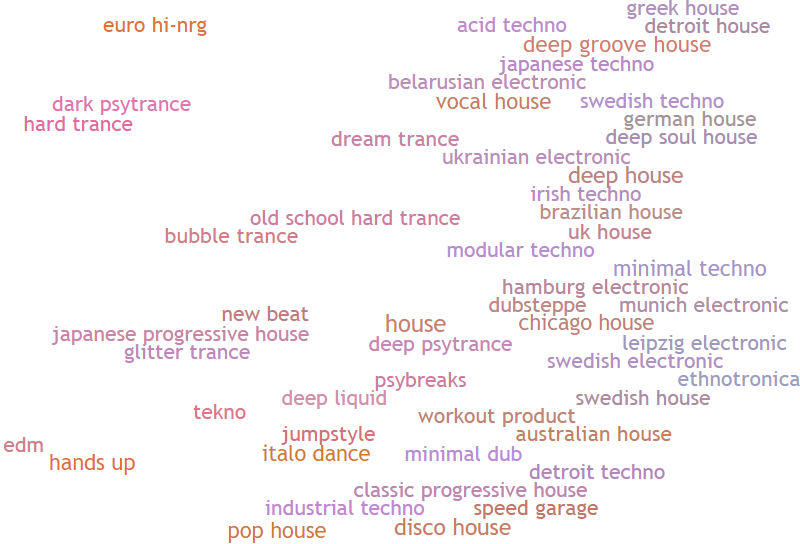
\includegraphics[width=0.8\textwidth]{images/everynoise.png}
        \caption{Minimalistická ukázka z obsáhlé poslouchatelné mapy hudebních žánrů.}
        \label{fig:everyNoise}
\end{figure}


% --------------------------------------------------------- %
\chapter{Generování fraktálů}

% Matematická definice tohoto pojmu zatím neexistuje. Nejblíže skutečnosti je patrně definice B. Mandelbrota:

% \begin{quote}
% "Fraktál je takový útvar, jehož Hausdorfova dimenze je větší než dimenze topologická."
% \end{quote}

% To znamená, že fraktál nemá jako krychle 3, či jako přímka 1 rozměr, ale jeho dimenze je neceločíselná. To nemusí platit vždy, např. Hilbertovy či Peanovy křivky vyplňují celou rovinu. Mimo Mandelbrotovy definice existuje i tzv. obecná definice podle níž je Fraktál je takový útvar, při jehož zvětšení dostaneme opět stejný obraz, bez ohledu na měřítko.
\begin{figure}[h]
    \centering
    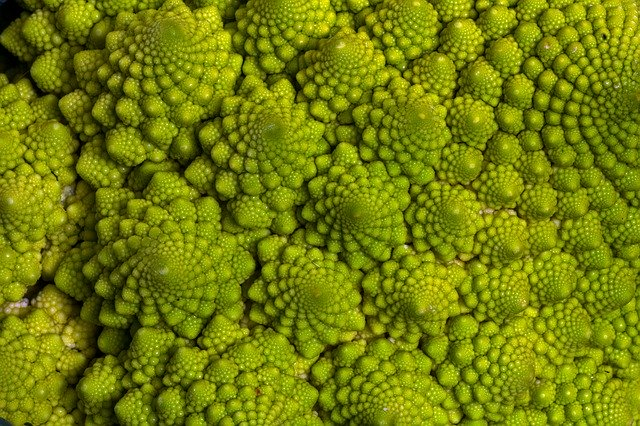
\includegraphics[width=220pt]{images/romanesco.jpg}
        \caption[Příklad fraktálu z přírody - zelenina romanesco.]{Příklad fraktálu z přírody - zelenina romanesco.}
        
        % https://farmarajecek.cz/detail/cz/nejkrasnejsi-zelenina-na-svete-romanesco-na-farme-rajecek

        \label{fig:romanesco}
\end{figure}


Fraktál je geometrický objekt, který po rozdělení na menší části vykazuje tvarovou podobnost s těmito částmi. Fraktálními objekty se zabývá samostatná vědní disciplína nazývaná fraktální geometrie \cite{resersePaus}. 


Fraktály jsou používané například pro modelování přírody a přírodních jevů (příklad na obrázku \ref{fig:romanesco}\footnote{Zdroj: \url{https://pixabay.com/cs/photos/zelenina-makro-květák-romanesco-659404/}}), inspirování se fraktálním uspořádání (fraktální antény, komprese dat atd.), či jen z estetických důvodů.

V této kapitole lze nalézt postupy generování fraktálů za účelem nalezení vhodných způsobů pro vizualizaci. Některé fraktály lze získat více postupy generování.
%Tato disciplína je intenzivně rozvíjena zhruba od šedesátých let minulého století. Za jejího zakladatele je dnes považován matematik Benoit B. Mandelbrot.

% \cite{Petyovsky}

\pagebreak



% https://www.youtube.com/watch?v=e0JaZuLfZ_0

% http://www.ksr.tul.cz/fraktaly/rozdeleni.html

\section{Programy pro generování fraktálů}

Pro počáteční inspiraci, jak se fraktály při generování chovají je možné vyzkoušet již existující software pro jejich vykreslování. Příkladem jsou specializované programy pro generování frakálů \textit{Chaotica}, \textit{Apophysis} a \textit{Mandelbulb 3D} pro trojdimenzionální fraktály (obrázek \ref{fig:mandelbulb}\footnote{Zdroj: \url{youtu.be/TTpbP5BVtiA}}). Generovat fraktály ale lze i grafickým programem \textit{GIMP} nebo dokonce v\textit{ MS PowerPoint}\footnote{Například tak, že slide odkazuje sám na sebe.}, pro zajímavost k vidění na obrázku \ref{fig:powerpoint}\footnote{Zdroj: \url{youtu.be/O8l_awjgoMI}}. 



\begin{figure}[h]
\centering
  \begin{subfigure}{0.55\textwidth}
    \includegraphics[width=\textwidth]{images/europa.png}
    \caption{Fraktály v \textit{Mandelbulb 3D}.}
    \label{fig:mandelbulb}
  \end{subfigure}
  \hspace{1pt}
  \begin{subfigure}{0.4\textwidth}
    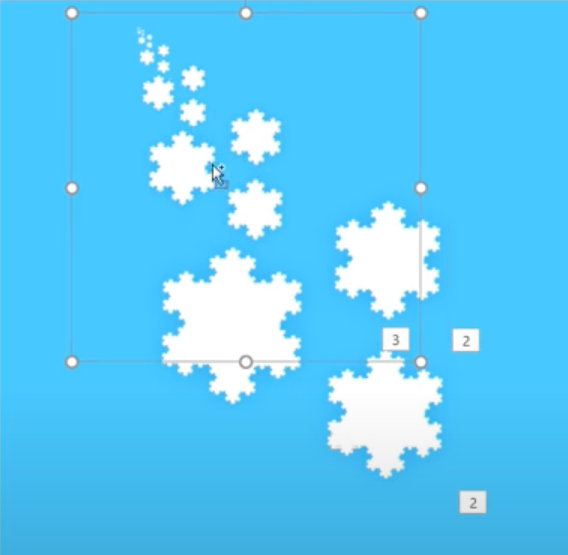
\includegraphics[width=\textwidth]{images/powerpoint.png}
    \caption{Fraktály v \textit{MS PowerPoint}.}
    \label{fig:powerpoint}
  \end{subfigure}
  
   
    \caption{ \label{fig:fractalPrograms}Generování fraktálů pomocí programů.}
\end{figure}


\note{V následujících poznámkách budou navrženy příklady způsobů, jak fraktály animovat a tím je využít pro hudební vizualizace. Triviálním způsobem, který může být aplikovaný pro řadu fraktálů je například prolínání výsledků iteračních kroků při konstrukci (což si lze představit jako časosběr při vykreslování).} 


% https://www.youtube.com/watch?v=O8l_awjgoMI


\section{IFS}

%  \todo[fancyline, color=green]{co takhle? (klidne smazte - nahore (92-102) je redefinice quote aby umela autory}


% \begin{quote}[Užití a zneužití fraktálů \cite{Wiesner}]{Robert Wiesner}
%   „Název IFS systémů je odvozen z původního anglického označení Iterated Function System, česky lze tento název přeložit jako systém iterovaných funkcí. První publikace, které se týkaly IFS systémů, vydali v roce 1985 Demko a následně pak v roce 1987 Barnsley. Tvorba obrázků pomocí IFS systémů patří mezi generativní metody vytváření fraktálů, kterou řadíme mezi metody deterministické. Algoritmus pro generování IFS fraktálů však může být jak deterministický, tak nedeterministický. Oboje paradoxně vede ke stejnému výslednému fraktálu, použijeme-li dostatečný počet iterací. Práce se systémy IFS představuje jednu z často používaných aplikací procedurálního modelování těles. Ve velkém množství případů se však jedná o pouhý podpůrný nástroj bez další návaznosti na celé trojrozměrné scény.“ 
% \end{quote}

% \cite{hajmova}

\textit{Iterated Function System}, neboli systém iterovaných funkcí je jedna z metod konstrukce fraktálů. Fraktály vznikají sjednocením několika kopií sama sebe, z nichž každá je transformovaná jinou funkcí ze systému. Tyto funkce jsou kontrahující, tj. obraz při této funkci je menší než jeho vzor. Celý fraktál je tedy složen z menších kopií sebe sama, které jsou také složeny z menších kopií sebe sama, atd. Je tedy soběpodobný.

Za transformační funkce se nejčastěji\footnote{Transformace mohou být i nelineární. Příkladem takových fraktálů je skupina \textit{Fractal flame}, které se dají vytvářet v již zmíněném programu \textit{Apophysis}.} používají afinní transformace, které provádějí s daným objektem následující operace: rotaci, zmenšování ve všech směrech a posun. Konstrukce IFS fraktálu znázorňuje \figurename~\ref{fig:ifsConstruction}\footnote{Zdroj: \url{https://en.wikipedia.org/wiki/Iterated_function_system}}. Efektivnějším algoritmem pro generování IFS fraktálů je stochastická metoda.

% Podle \cite{sixta} existuje několik způsobů generování. Na obrázcích \ref{fig:trisection} a \ref{fig:chaosGame} jsou různé způsoby generování Sierpińského trojúhelníka. Prvním z nich je stochastický způsob, někdy nazývaný chaotická hra.

\begin{figure}[h]
    \centering
    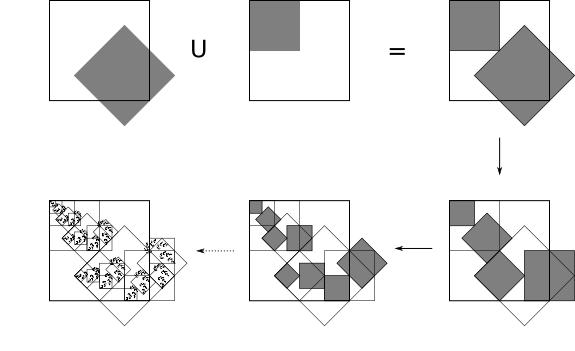
\includegraphics[width=0.8\textwidth]{images/Ifs-construction.png}
        \caption{Konstrukce fraktálu pomocí IFS.}
    \label{fig:ifsConstruction}
\end{figure}

\subsection*{Stochastická metoda}

Fraktál vzniká z počátečního bodu, na který se aplikuje sada transformačních pravidel. Jednotlivým pravidlům se přiřazuje určitá pravděpodobnost, pravidlo tudíž vybírá náhodnou (stochastickou) cestou. Podle \cite{sixta} se algoritmus někdy nazývá chaotická hra.

\begin{figure}[h]
    \centering
    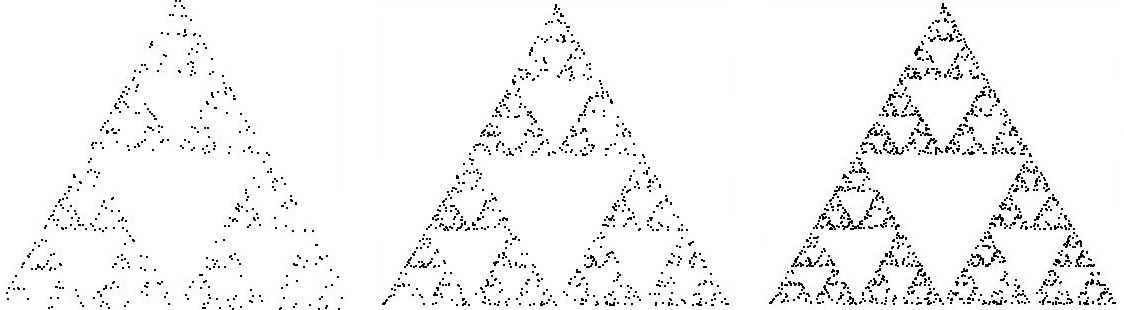
\includegraphics[width=0.9\textwidth]{images/sierpinskyChaos.jpg}
        \caption{Sierpińského trojúhelník pomocí chaotické hry. Výsledky po 500, 1000 a 2000 krocích.}
    \label{fig:chaosGame}
\end{figure}

\newpage

Jednotlivá transformační pravidla lze označit jako funkce  $w_{1},w_{2},w_{3},\ldots,w_{n}$, kde každé funkci se přiřadí pravděpodobnost $p_{1},p_{2},\ldots,p_{n}$. Jejich součet dává 1 (100\%). Funkce $w_i$ se dá matematicky vyjádřit rovnicí \ref{eq:3}, kde  $x, y$ jsou souřadnice bodu, parametry $a, b, c, d$ určují rotaci a parametry $e, f$ translaci\footnote{Přesnější popis parametrů lze nalézt například zde: \cite{bourke}, \cite{itnetwork}.}

\begin{equation} \label{eq:3}
{\displaystyle 
    w_i\begin{pmatrix}x\\y\end{pmatrix} = 
    \begin{pmatrix}a&b\\c&d\end{pmatrix}\begin{pmatrix}x\\y\end{pmatrix}+\begin{pmatrix}e\\f\end{pmatrix}
    } \enspace .
\end{equation}


Nový bod se stává opět počátkem pro další transformaci. Výsledek je obdržen po několika tisících iterací. Průběžné výsledky konstrukce Sierpińského trojúhelníku pomocí této metody je vidět na obrázku \figurename~\ref{fig:chaosGame}\footnote{Zdroj: \url{https://thatsmaths.com/2014/05/22/the-chaos-game/}}.





% Intuitivnější způsob konstrukce je iterativní metoda. Spočívá v aplikaci geometrických pravidel na nějaký základní obrazec (například trojúhelník a čtverec). Sierpińského trojúhelník lze zkonstruovat z počátečního vyplněného trojúhelníka vyjmutím trojúhelníka, který vznikne spojením středů stran původního trojúhelníka. Na nově vzniklé trojúhelníky se opakovaně aplikuje stejné pravidlo, jak je ukázáno na obrázku \ref{fig:trisection}.

% http://paulbourke.net/fractals/ifs/

% $a = r_1*cos(\phi), $
% $b = r_2*sin(\theta), $
% $c = -r_1*sin(\phi) $ a
% $d = r_2*cos(\phi) $ . 
% Podle  jsou úhly $\phi$ a $\theta$ otočení na osách \textit{x}
%  a \textit{y} přeškálované o parametry $r_1$ a $r_2$. Parametr $e$ je horizontální translace a parametr $f$ vertikální translace.

\begin{figure}[h]
\centering
    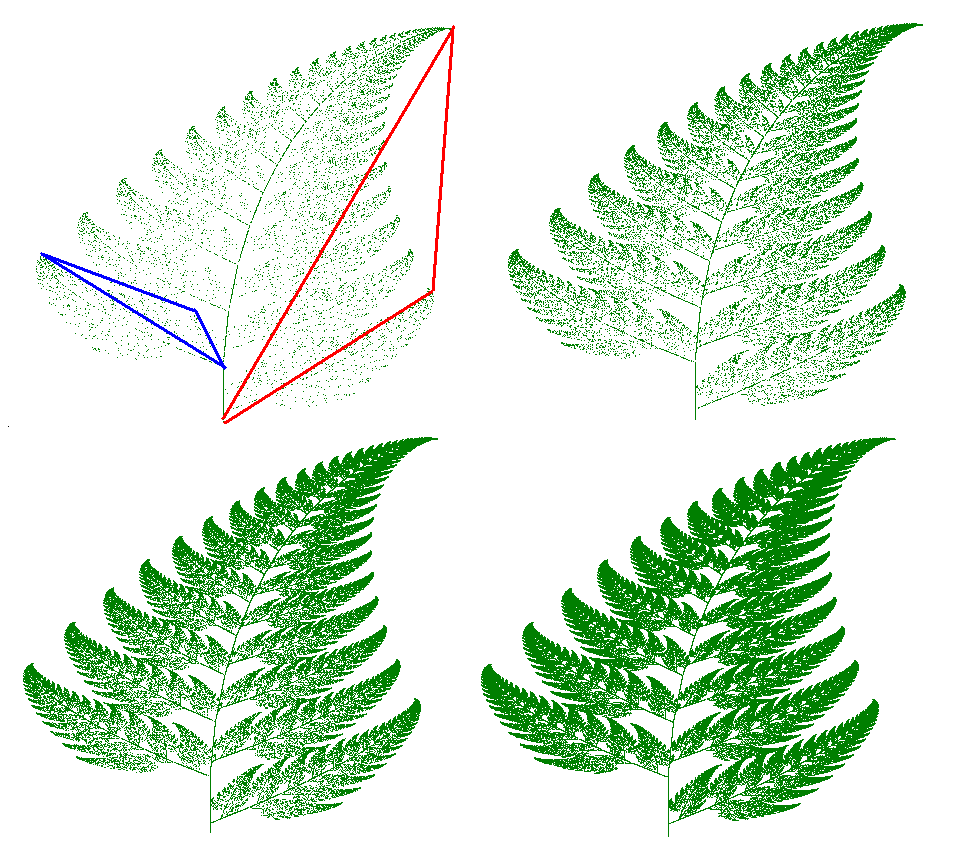
\includegraphics[width=0.9\textwidth]{images/barnsley.png}
      \caption{ \label{fig:fern}Generování fraktálů pomocí stochastického IFS.}
\end{figure}

\newpage

\begin{table}[h]
%   \begin{subtable}[]{1.0\linewidth}%
   \centering%
\begin{tabular}{@{}cccccc@{}}
\toprule
\textbf{} & \textbf{$w_1$} & \textbf{$w_2$} & \textbf{$w_3$} & \textbf{$w_4$} \\ \midrule
a         & 0.0            & 0.2            & -0.15          & 0.85           \\
b         & 0.0            & -0.26          & 0.28           & 0.04           \\
c         & 0.0            & 0.23           & 0.26           & -0.04          \\
d         & 0.16           & 0.22           & 0.24           & 0.85           \\
e         & 0.0            & 0.0            & 0.0            & 0.0            \\
f         & 0.0            & 1.6            & 0.44           & 1.6            \\
p         & 0.01           & 0.07           & 0.07           & 0.85           \\ 
generovaná část         & stonek           & levý list           & pravý list           &  menší lístky           \\ \bottomrule
\end{tabular}
%   \caption[]{Parametry funkcí pro kapradí.}

% \end{subtable}%
%   \begin{subtable}[]{1.0\linewidth}
% \centering
% \begin{tabular}{@{}cccccc@{}}
% \toprule
% \textbf{} & \textbf{$w_1$} & \textbf{$w_2$} & \textbf{$w_3$} \\ \midrule
% a         & 0.387          & 0.441          & -0.468         \\
% b         & 0.430          & -0.091         & 0.020          \\
% c         & 0.430          & -0.009         & -0.113         \\
% d         & -0.387         & -0.322         & 0.015          \\
% e         & 0.2560         & 0.4219         & 0.4            \\
% f         & 0.5220         & 0.5059         & 0.4            \\
% p         & 1/3            & 1/3            & 1/3            \\ \bottomrule
% \end{tabular}
%  \caption[]{Parametry funkcí pro větev.}

%   \end{subtable}
  \caption{\label{table:ifs}Příklady parametrů pro generování Barnsleyho kapradí.}
\end{table}

 Příklad parametrů ukazuje \tablename~\ref{table:ifs}. Tyto parametry generují známé Barnsleyho kapradí pojmenované po Michaelu Barnsleym, který jako první popsal tento fraktál ve své knize \cite{barnsley}. Zmíněnou pravděpodobnost\footnote{Lze se domnívat, že je to z důvodu rozložení překreslovacích pravidel (které nemusí být rovnoměrné). Kdyby všech $n$ iterací připadlo jednomu z pravidel, nebylo by dosaženo požadovaného výsledku, neb každé z pravidel by se dalo vykreslovat donekonečna.} udává v tabulce parametr $p$.
 
 \figurename~\ref{fig:fern}\footnote{Zdroj: \url{http://paulbourke.net/fractals/ifs/}} znázorňuje postupné generování Barnsleyho kapradí podle parametrů z tabulky.  \figurename~\ref{fig:fernStem} pro zajímavost ilustruje obměnu parametrů, konkrétně nenulový parametr $a$ vykreslující stonek, zapříčiňující vykreslování malého listu místo stonku.

\begin{figure}[h]
\centering
    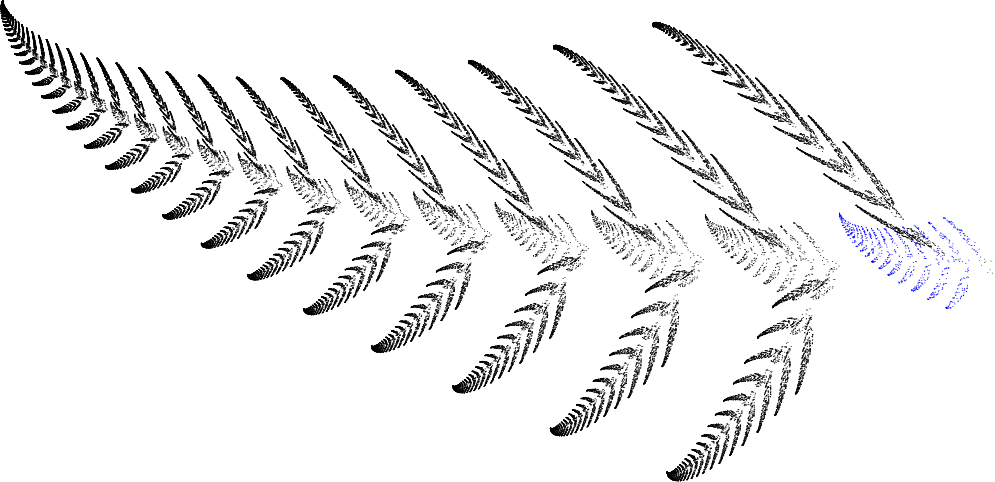
\includegraphics[width=0.5\textwidth]{images/fernA.png}
      \caption[Bernsleyho kapradí s nenulovým parametrem $a$.]{ \label{fig:fernStem}Bernsleyho kapradí s nenulovým parametrem $a$ (obrázek je otočen).}
\end{figure}


% \vspace{5pt}

% \begin{figure}[h]
%     \centering
%     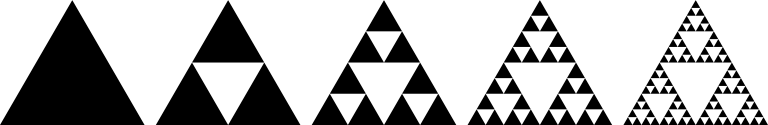
\includegraphics[width=0.7\textwidth]{images/sierpinskyGeometry.png}
%         \caption{Iterativní konstrukce Sierpińského trojúhelníka.}
%     \label{fig:trisection}
% \end{figure}


\hspace{5cm}



\note{Pro animace IFS fraktálů je možné upravovat hodnoty pravidel přidáním závislosti nějakého z parametrů na čase (například těch, upravujících rotaci).}
    
% \begin{figure}[ht]
%     \begin{minipage}[b]{0.45\linewidth}
%         \centering
%         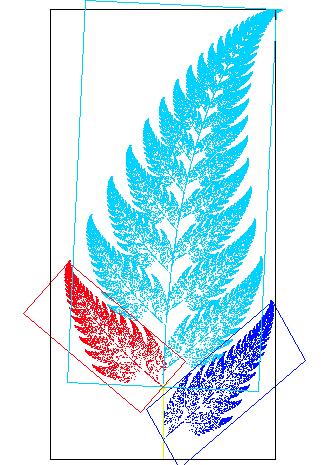
\includegraphics[width=\textwidth]{images/ifs1.png}
%         \caption{Fractal fern}
%         \label{fig:fern}
%         \end{minipage}
%         \hspace{0.5cm}
%         \begin{minipage}[b]{0.45\linewidth}
%         \centering
%         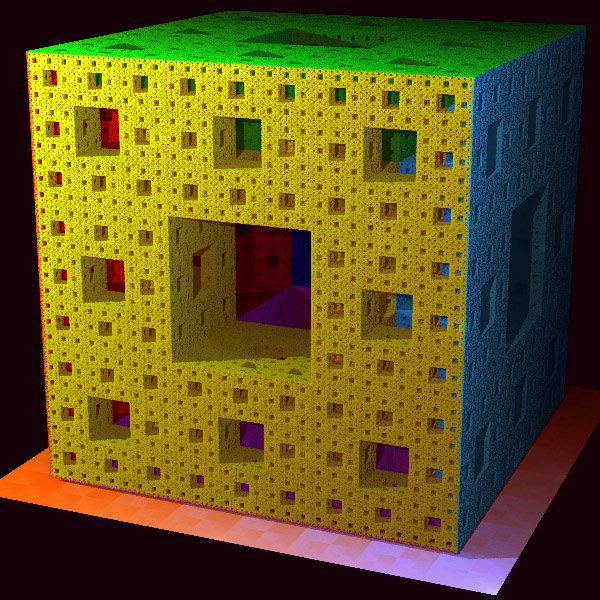
\includegraphics[width=\textwidth]{images/ifs2.jpg}
%         \caption{Menger sponge}
%         \label{fig:sponge}
%         \end{minipage}
% \end{figure}


% https://en.wikipedia.org/wiki/Iterated_function_system

% use fixed geometric replacement rules; may be stochastic or deterministic;[45] e.g., Koch snowflake, Cantor set, Haferman carpet,[46] Sierpinski carpet, Sierpinski gasket, Peano curve, Harter-Heighway dragon curve, T-square, Menger sponge


% \section{Chaos game}

% Fraktály IFS mohou být konstruovány i jiným způsobem. Termín \textit{chaos game} se v matematice původně odkazoval na metodu generování fraktálu s využitím polygonu a počátečního bodu na náhodné pozici uvnitř polygonu. Fraktál je vytvářen iterativním generováním sekvece bodů, původně začínající v počátečním náhodném bodě, ve kterém každý bod sekvence je dán zlomkem vzdálenosti mezi bodem předchozím a jedním z vrcholů polygonu. Vrchol je vybrán náhodně v každé iteraci. Opakováním tohoto iteračního procesu, náhodným výběrem vrcholu při každé iteraci a vyhazováním prvních několika bodů ze sekvence se často (ale ne vždy) vytvoří fraktální tvar. Použitím pravidelného trojúhelníku a faktoru 1/2 vznikne Sierpinského trojúhelník, zatímco vhoné uspořádání se čtyřmi body a faktorem 1/2 vytvoří Sierpinského čtyřstěn, trojrozměrnou analogii Sierpinského trojúhelníku. Příklad na obrázku \ref{fig:sierpinski}\footnote{Zdroj: https://thatsmaths.com/2014/05/22/the-chaos-game/}.

% In mathematics, the term chaos game originally referred to a method of creating a fractal, using a polygon and an initial point selected at random inside it. The fractal is created by iteratively creating a sequence of points, starting with the initial random point, in which each point in the sequence is a given fraction of the distance between the previous point and one of the vertices of the polygon; the vertex is chosen at random in each iteration. Repeating this iterative process a large number of times, selecting the vertex at random on each iteration, and throwing out the first few points in the sequence, will often (but not always) produce a fractal shape. Using a regular triangle and the factor 1/2 will result in the Sierpinski triangle, while creating the proper arrangement with four points and a factor 1/2 will create a display of a "Sierpinski Tetrahedron", the three-dimensional analogue of the Sierpinski triangle. As the number of points is increased to a number N, the arrangement forms a corresponding (N-1)-dimensional Sierpinski Simplex. WIKIPEDIA



% https://www.johndcook.com/blog/2017/07/08/the-chaos-game-and-the-sierpinski-triangle/

\newpage

\section{Kaleidoskopické IFS}\label{kaleidoscope}


V různých zdrojích (například \cite{fractalForums,roy}) lze nalézt konstrukci fraktálu pomocí iterativního přehýbání prostoru, nazvané Kaleidoscopic (kaleidoskopické) IFS.

Na obrázku \ref{fig:koch}\footnote{Zdroj: \url{http://datagenetics.com/blog/january12016/index.html}} je znázorněna klasická iterativní konstrukce Kochovy vločky. Kochova vločka vygenerovaná přehýbáním a zrcadlením prostoru je na obrázku \ref{fig:folding}. Výhody tohoto komplikovanějšího způsobu se projeví při aplikaci libovolné textury (například \ref{fig:london}), která po překládání prostoru vytvoří zajímavé obrazce (například \ref{fig:kaleidoskop}\footnote{Zdroj: \url{youtu.be/il_Qg9AqQkE}}), objasňující výraz kaleidoskopické.



% Kaleidoscopic (escape time) IFS. Příklad na obrázku \ref{fig:kifs}\footnote{Zdroj: http://www.fractalforums.com/sierpinski-gasket/kaleidoscopic-(escape-time-ifs)/80/}.

\begin{figure}[h]
    \centering
    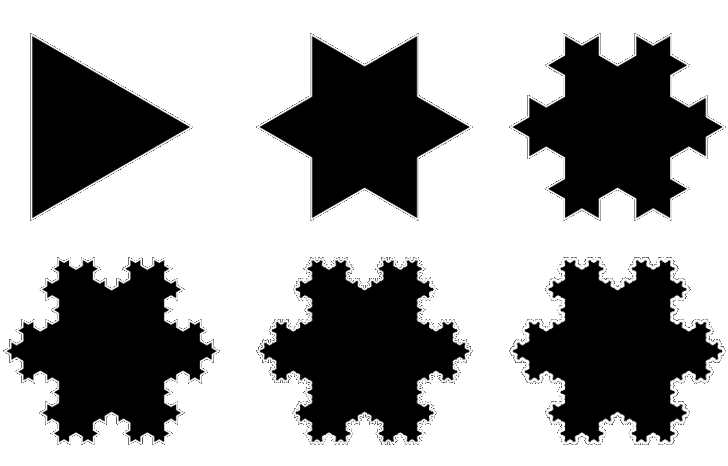
\includegraphics[width=200pt]{images/kp.png}
    % http://www.fractalforums.com/sierpinski-gasket/kaleidoscopic-(escape-time-ifs)/80/
        \caption{Iterativní konstrukce Kochovy vločky.}
        \label{fig:koch}
\end{figure}

\begin{figure}[h]

\centering

\mbox{
  \begin{subfigure}{0.27\textwidth}
    
\includegraphics[width=\textwidth]{images/koch_folding2.png}
    \caption{Kochova vločka.}
    \label{fig:folding}
  \end{subfigure}
}
\hspace{1pt}
\mbox{
  \begin{subfigure}{0.27\textwidth}
    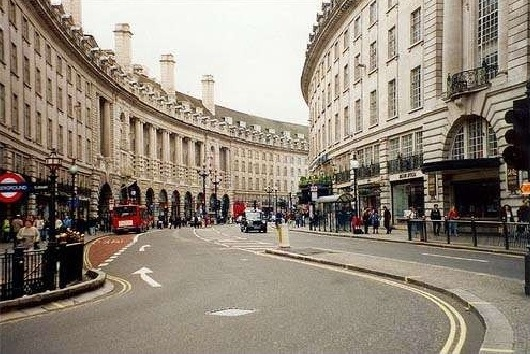
\includegraphics[width=\textwidth]{images/london.jpg}
    \caption{Foto z Londýna}
    % https://www.slideshare.net/theringgirl/london-cbd
    \label{fig:london}
  \end{subfigure}
}
\hspace{1pt}
\mbox{
  \begin{subfigure}{0.27\textwidth}
    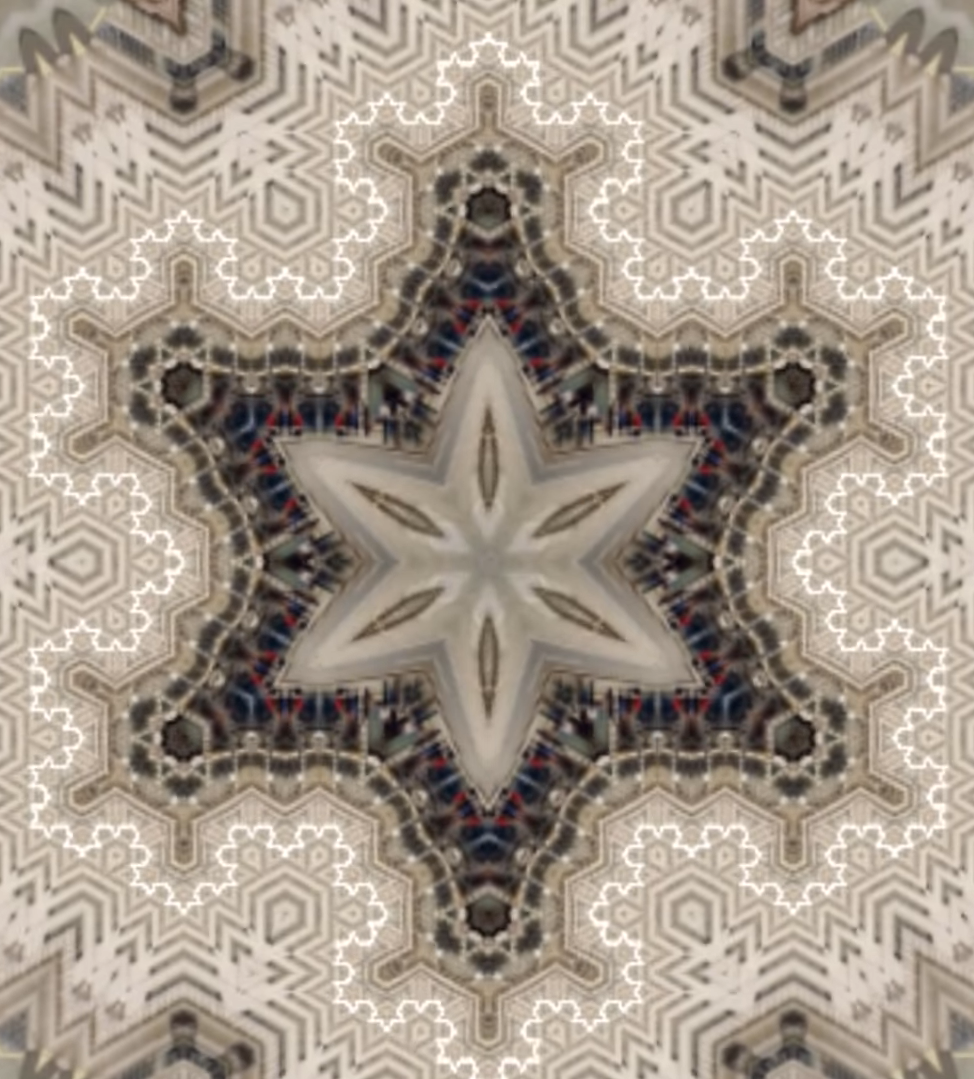
\includegraphics[width=\textwidth]{images/koch_folding3.png}
    \caption{Aplikace textury.}
    \label{fig:kaleidoskop}
  \end{subfigure}
}
   
    \caption{ \label{fig:kifs}Aplikace textury na kaleidoskopický IFS fraktál.}
    % \caption{ \label{fig:predecessors}.}
\end{figure}

\vspace{5pt}

\note{Fraktály tohoto typu mohou být animované například posunováním textury (či obecně obsahem zpřehýbaného prostoru), nebo změnou definic přehybání prostoru (přesně tak, jak funguje kaleidoskop).}
    
    
\newpage

% \subsection*{Hybridní 3D fraktály}

% A lot of great images have been made of the Mandelbulb, the Mandelbox, and the various kaleidoscopic IFS’s (the non-platonic non-solids). And it turns out that by combining these formulas (and stirring a few assorted functions into the mix), a variety of new, amazing, and surprising forms emerge.

% http://blog.hvidtfeldts.net/index.php/2010/04/folding-space-the-mandelbox-fractal/
% https://sites.google.com/site/mandelbox/what-is-a-mandelbox

% A multifractal system is a generalization of a fractal system in which a single exponent (the fractal dimension) is not enough to describe its dynamics; instead, a continuous spectrum of exponents (the so-called singularity spectrum) is needed.[1

% \newpage

\section{L-Systémy}

% use string rewriting; may resemble branching patterns, such as in plants, biological cells (e.g., neurons and immune system cells[26]), blood vessels, pulmonary structure,[47] etc. or turtle graphics patterns such as space-filling curves and tilings

L-systém nebo také Lindenmayerův systém je varianta formální gramatiky, vyvinutá pro modelování růstu rostlin. L-Systém je formálně definován trojicí $G=(\Sigma, S, P)$. Kde  $\Sigma$ je abeceda (neprázdná množina symbolů), $S$ je axiom (konečné slovo z abecedy definující počáteční stav systému) a $P$ je množina přepisovacích pravidel. Za bibli L-systémů se považuje kniha \cite{Lsys}, kterou publikoval Lindenmayer spolu s Prusinkiewiczem.


% Název L-systémy vznikl buďto z anglického sousloví LOGO-like turtle, nebo podle botanika Aristida Lindenmayera, který je použil již v roce 1968 pro simulaci vývoje mnohobuněčných organismů. Takže v některé literatuře jsou také označovány termínem Lindenmayerovy systémy. Pro L-systémy se někdy používá i označení fraktální křivky. Nicméně LOGO je programovací jazyk, ve kterém se pomocí jednoduchých příkazů dají pomocí želvy kreslit různé obrazce. Podstatou tvorby L-systémů je přepisování řetězců podle určitých pravidel (gramatik). Každému terminálnímu symbolu (znaku, jež se nepřepisuje) v řetězci je přiřazen jistý geometrický význam, například transformace či generování objektu.  \cite{Wiesner}

\begin{table}[h]
\centering
\begin{tabular}{@{}cccccc@{}}
\toprule
\multicolumn{2}{l}{\cellcolor[HTML]{F2F2F2}{\color[HTML]{202122} \textbf{gramatika}}}    \\ \midrule
{ \textbf{abeceda:}}           & {\color[HTML]{202122} F + -}        \\
{\textbf{axiom:}}             & {\color[HTML]{202122} F}            \\
{ \textbf{přepis. pravidla:}}  & {\color[HTML]{202122} F → F+F--F+F} \\ \midrule
\multicolumn{2}{l}{\cellcolor[HTML]{F2F2F2}{\color[HTML]{202122} \textbf{interpretace}}} \\ \midrule
{ \textbf{úhel otočení:}}      & {\color[HTML]{202122} 60°}         
\end{tabular}
\caption[L-systém - příklad pravidel pro tvorbu Kochovy křivky.]{ \label{table:lsys}L-systém - příklad pravidel pro tvorbu Kochovy křivky. Znaménka $+$ a $-$ reprezentují otočení doleva, či doprava. Axiom $F$ je instrukce pro nakreslení úsečky.}
\end{table}

V tabulce \ref{table:lsys} je příklad L-systému pro tvorbu Kochovy křivky (části Kochovy vločky, jejíž konstrukce pomocí jiných postupů byly popsány výše). Na obrázku \ref{fig:lsysKoch}\footnote{Zdroj: \url{https://cs.wikipedia.org/wiki/L-systém}} je shora znázorněna 0., 1., 2. a 3. generace vygenerovaná pomocí těchto pravidel.


\begin{figure}[h]
    \centering
    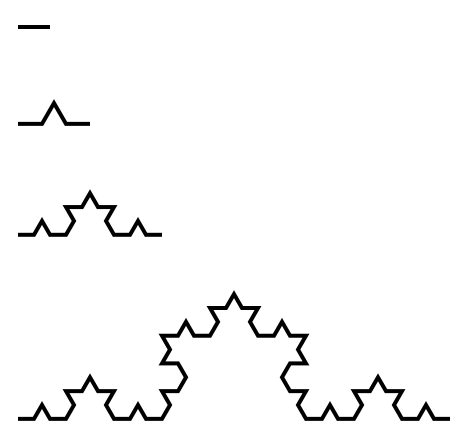
\includegraphics[width=150pt]{images/koch.png}
        \caption{Kochova křivka vygenerovaná pomocí L-systému.}
        \label{fig:lsysKoch}
\end{figure}



\note{Fraktály získané pomocí L-systémů lze animovat například upravováním úhlu v přepisovacích pravidlech.}


% L-systémy, v minulosti též známé pod názvem Lindenmayerovy systémy, jsou skupinou fraktálů definovaných ve své nejjednodušší podobě pomocí regulárních nebo bezkontextových přepisovacích gramatik. \cite{root}

%\begin{figure}[htbp]
%    \centering
%    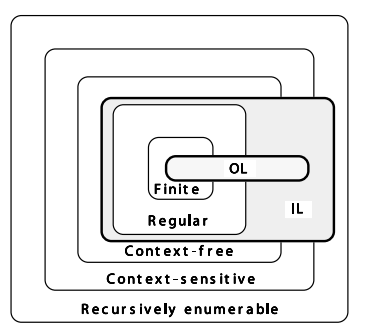
\includegraphics[scale=1]{images/chomsky_difference.png}
%        \caption[]{\label{}Relations between Chomsky classes of languages and language classes generated by L-systems. The symbols OL and IL denote language classes generated by context-free and context-sensitive L-systems, respectively.}
%\end{figure}


% http://algorithmicbotany.org/papers/algorithms-for-inferring-context-sensitive-l-systems.pdf

% Biomimetika je obor vědy, který zkoumá zajímavá konstrukční řešení v přírodě u živých organismů a snaží se je napodobit a využít k vývoji nových vynálezů, technických řešení a jejich široké využití pro pokrok atd. Wikipedie

\section{Využití chaosu a dynamiky}

%%%%%%%%%%%%% Puvodni verze::::::::::::::::::

% \subsection*{Atraktor}

% Atraktor\footnote{Zdroje čerpání: \cite{resersePaus} \cite{Wiesner} \cite{root3}.} dynamického systému je množina stavů, do kterých systém směřuje. Jedná se o množinu hodnot, kterých může nabývat stavový vektor dynamického systému po dostatečně dlouhém časovém úseku od počátečního impulsu. Atraktory lze dělit do několika skupin.
% % http://geraldine.fjfi.cvut.cz/~pausp/clanek/reserse
% % http://www.hungry-lord.wz.cz/data/chaos.php
% % https://www.root.cz/clanky/fraktaly-v-pocitacove-grafice-iii/


% \begin{description}
%     \item [Atraktorem jsou pevné body.] Systém se v nekonečném čase ustálil v nějakém stabilním stavu, který lze dopředu vypočítat.
%     \item [Atraktorem jsou periodické body.] Systém se ustálil tak, že osciluje mezi několika stavy.
%     \item [Atraktorem jsou kvaziperiodické body.] Systém rovněž osciluje mezi několika stavy.
%     \item [Chaotický atraktor] mají dynamické systémy jejichž výsledný stav systému nelze v podstatě nijak dopředu předpovědět, například protože je systém velmi citlivý na počáteční podmínky.
%     \item [Podivný atraktor] je z hlediska fraktální geometrie nejzajímavějším případem atraktoru. Tento typ atraktoru může vzniknout tehdy, je-li systém popsán minimálně třemi diferenciálními rovnicemi\footnote{V případě, že funkce použité v rovnicích není možné invertovat, může být rovnic i méně – příkladem je bifurkační diagram.}. Takový systém může mít velmi komplikovaný atraktor, který sice bude vykazovat vlastnosti pravidelného, ale současně i chaotického atraktoru.
% \end{description}


% \begin{quote}[Užití a zneužití fraktálů \cite{Wiesner}]{Robert Wiesner}
% "Dynamické systémy s fraktální strukturou existují i v komplexní rovině. Z těchto systémů jsou asi nejvíce známé \textit{Juliovy množiny} a \textit{Mandelbrotova množina}. Existuje i rozšíření Juliových množin a Mandelbrotovy množiny do hyperkomplexního prostoru. Dalším notoricky známým příkladem dynamického systému je \textit{Lorenzovo vodní kolo}. Existují i jiné fraktály generované pomocí dynamických systémů, například \textit{King’s dream}, který vymyslel Clifford Pickover čistě z estetického hlediska."
% \end{quote}


% https://www.sfu.ca/~rpyke/335/summary.html
% https://www.sfu.ca/~rpyke/335/summary.html
% https://www.sfu.ca/~rpyke/335/summary.html
% https://www.sfu.ca/~rpyke/335/summary.html
% https://www.sfu.ca/~rpyke/335/summary.html

%%%%%%%%%%%%% Nova verze::::::::::::::::::

Dynamický systém je matematický model, jehož stav je závislý na nějaké nezávislé veličině (nejčastěji to bývá čas). Je popsán pomocí dynamických podmínek, které popisují změnu tohoto systému v čase. Stav systému v libovolném časovém okamžiku je reprezentován stavovým vektorem.

% \footnote{Zdroje čerpání: \cite{resersePaus} \cite{Wiesner} \cite{root3}.}
Atraktor dynamického systému je množina stavů, do kterých systém směřuje. Jedná se o množinu hodnot, kterých může nabývat stavový vektor dynamického systému po dostatečně dlouhém časovém úseku od počátečního impulsu. 

Teorie chaosu\footnote{Chaos se v tomto kontextu myslí stochastické chování v deterministickém systému, neboli nepravidelné chování podle přesných pravidel. Zdroj: \cite{Stewart2009}.} vysvětluje proč některé fenomény jsou nepředvídatelné, i přesto, že jsou popsané matematickými rovnicemi. Fraktály jsou nekonečně členité geometrické objekty a tím tedy nekonečně komplexní. Podivné atraktory jsou spojením mezi chaosem a fraktály. Skutečnost, že dynamické systémy mají atraktory (anglicky \textit{attractor}, z původně latinského \textit{attrahere} - přitahovat) by se řečnicky dala vyjádřit tak, že atraktory přitahují řešení (nakonec tedy řešení bude tak komplikované jako samotný atraktor). Podivné atraktory mají tuto fraktální strukturu a jsou proto nekonečně komplikované.\footnote{Text volně přeložen z \cite{pyke}.}



\begin{quote}[Užití a zneužití fraktálů \cite{Wiesner}]{Robert Wiesner}
\uv{Dynamické systémy s fraktální strukturou existují i v komplexní rovině. Z těchto systémů jsou asi nejvíce známé \textit{Juliovy množiny} a \textit{Mandelbrotova množina}. Existuje i rozšíření Juliových množin a Mandelbrotovy množiny do hyperkomplexního prostoru. Dalším notoricky známým příkladem dynamického systému je \textit{Lorenzovo vodní kolo}. Existují i jiné fraktály generované pomocí dynamických systémů, například \textit{King’s dream}, který vymyslel Clifford Pickover čistě z estetického hlediska.}
\end{quote}

% https://www.youtube.com/watch?v=vfteiiTfE0c
% https://www.youtube.com/watch?v=vfteiiTfE0c
% https://www.youtube.com/watch?v=vfteiiTfE0c

\subsection*{Juliovy množiny}

Juliovy\footnote{Byly poprvé popsány Gastonem Juliou a Pierrem Fatouem.} množiny mohou být vytvářeny pomocí iterace funkce komplexní paraboly \ref{eq:julia}. Vygenerovat Juliovu množinu lze zvolením komplexního čísla $c$, které se pro jeden obrazec nemění. Následně pro každý bod komplexní roviny $z$ nutno zjistit, zda neustálým mocněním bodu $z$ a přičítáním konstanty $c$ diverguje. Pokud nediverguje, patří bod do množiny. 

\begin{equation} \label{eq:julia}
    {\displaystyle z_{n+1}=z_{n}^2+c}\enspace .
\end{equation}

% V praxi vypadá výpočet velmi snadno: Zkoumané číslo $z$ je umocněno a je k němu přičtena konstanta $c$. Pokud je výsledek v absolutní hodnotě větší než 2, bod nepatří do množiny. Pokud je menší, zopakuje se výpočet. Jestliže ani po několika iteracích nepřesáhne výsledek hodnotu 2, patří bod do Juliovy množiny. Na počtu provedených iterací (v ideálním případě nekonečno) závisí ostrost detailů zobrazené množiny. Podle počtu iterací, po kterých absolutní hodnota bodu z překročí 2, lze danému bodu přiřadit barvu a získat tak různé barevné přechody.

\subsection*{Mandelbrotova množina}

Mandelbrotova množina je narozdíl od Juliových množin\footnote{Volbou jiného komplexního čísla $c$ vznikne jiný obraz Juliovy množiny. Juliovy množiny mohou být generovány jiným předpisem.} jen jedna. K jejímu určení se používá zobrazení, které každému komplexnímu číslu $c$ přiřazuje určitou posloupnost komplexních čísel $z_{n}$. Tato posloupnost je určena následujícím rekurzivním předpisem:

\begin{equation} \label{eq:mandelbrot}
    {\displaystyle z_0=0,\enspace z_{n+1}=z_{n}^2+c}\enspace .
\end{equation}

Mandelbrotova množina je pak definována jako množina komplexních čísel $c$, pro která je posloupnost $z_{0},z_{1},z_{2},\dots$   omezená, tj. splňuje následující podmínku: existuje reálné číslo $m$ takové, že pro všechna $n$ je $|z_n| \leq m$. 


Mandelbrotova množina lze ovšem také definovat jako množina všech komplexních čísel $c$, kdy je Juliova množina $J_c$ souvislá. Tento vztah ukazuje \figurename~\ref{fig:js3}\footnote{Zdroj: \url{youtu.be/vfteiiTfE0c}}, kde je na levé straně Mandelbrotova množina a na pravé straně Juliova množina.



\begin{figure}[h]
    \centering
    \noindent
    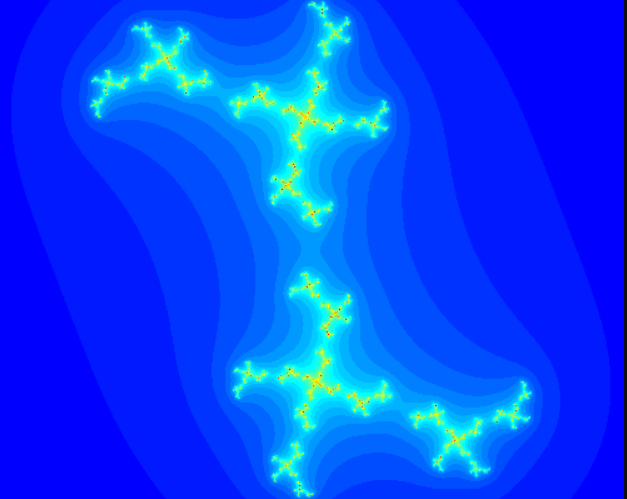
\includegraphics[width=0.3\textwidth]{images/julia1.png}\hspace{0.05\textwidth}%
    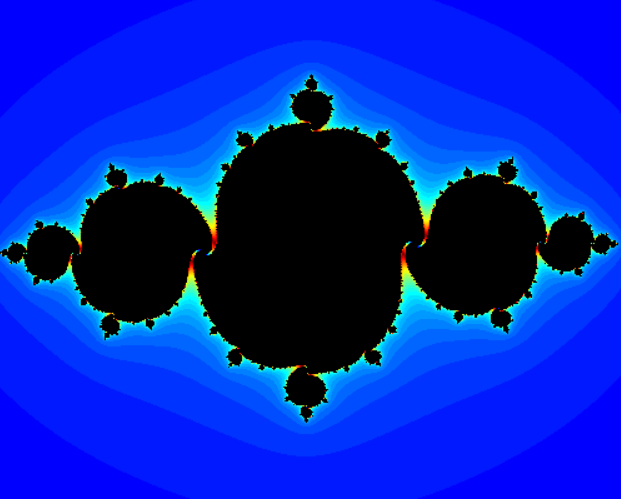
\includegraphics[width=0.3\textwidth]{images/julia35.png}\\[1em]
    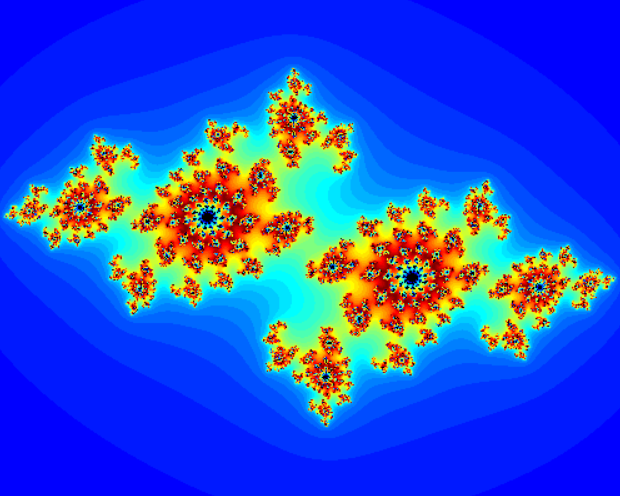
\includegraphics[width=0.3\textwidth]{images/julia36.png}\hspace{0.05\textwidth}%
    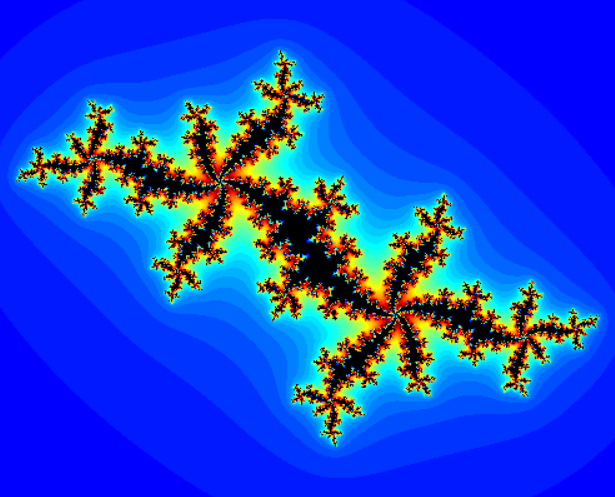
\includegraphics[width=0.3\textwidth]{images/julia4.png}\par
    \caption{Animace Juliových množin pomocí vztahu $fc(z)=z^2+C$.}
    \label{fig:julia}
\end{figure}

\note{Fraktály obdržené pomocí dynamických systémů vybízí pro animace použít veličinu, na které systém závisí - tedy často čas.}

\note{Juliovy množiny lze animovat volbou komplexního čísla $c$, například deklarováním $c = 0.7885\,e^{ia}$, kde $a$ nabývá hodnot od $0$ do $2\pi$. Průběh animace ukazuje \figurename~\ref{fig:julia}.}



% \footnote{Zdroj: \url{https://cs.wikipedia.org/wiki/Juliova_množina}}. 

\begin{figure}
\centering
  \begin{subfigure}[b]{1.0\textwidth}
    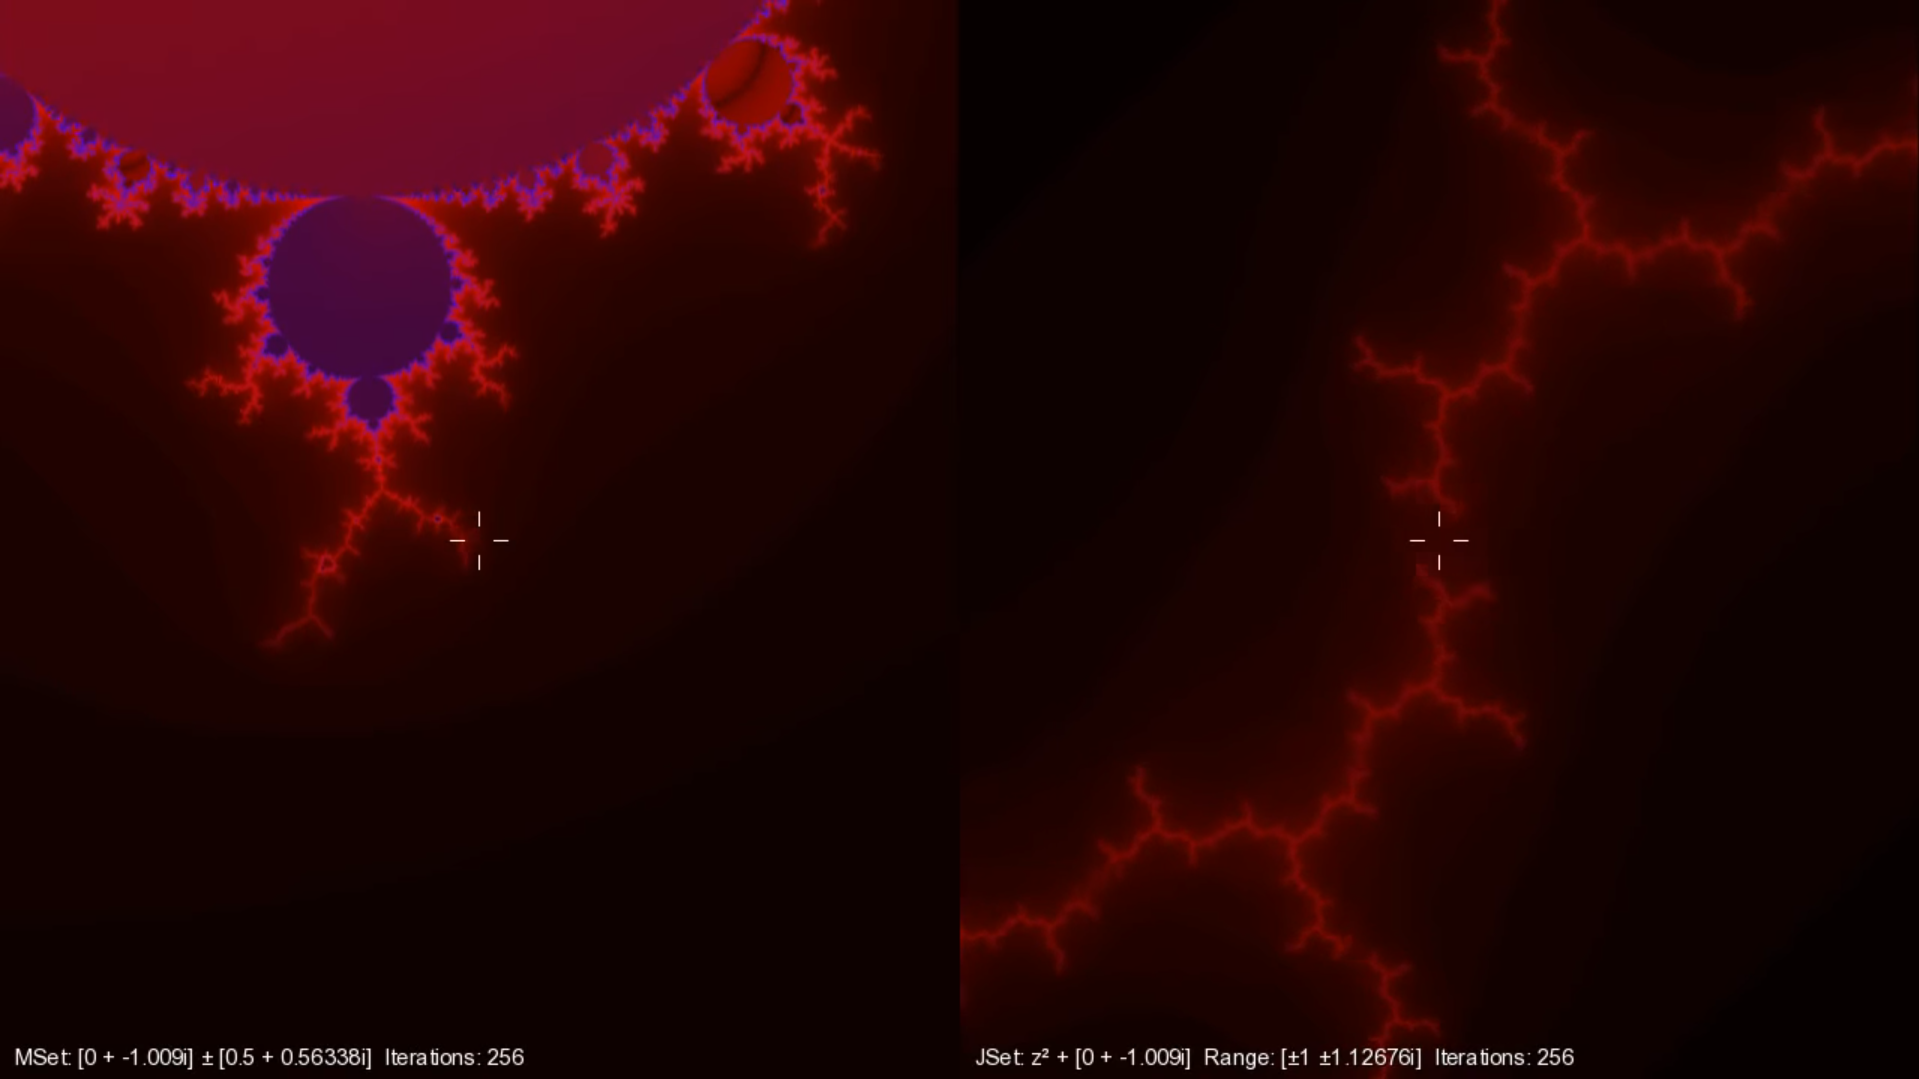
\includegraphics[width=\textwidth]{images/jmsets2.png}
    \caption[]{\label{fig:js1}MSet: $[0 + -1.009i]\pm[0.5+0.56338i]$ Iterace: $256$.\\JSet: $z^2+[0 + -1.009i]$ Range: $[\pm1 \pm1.12676i]$ Iterace: $256$.}
  \end{subfigure}
  \vspace{5pt}
  \begin{subfigure}[b]{1.0\textwidth}
    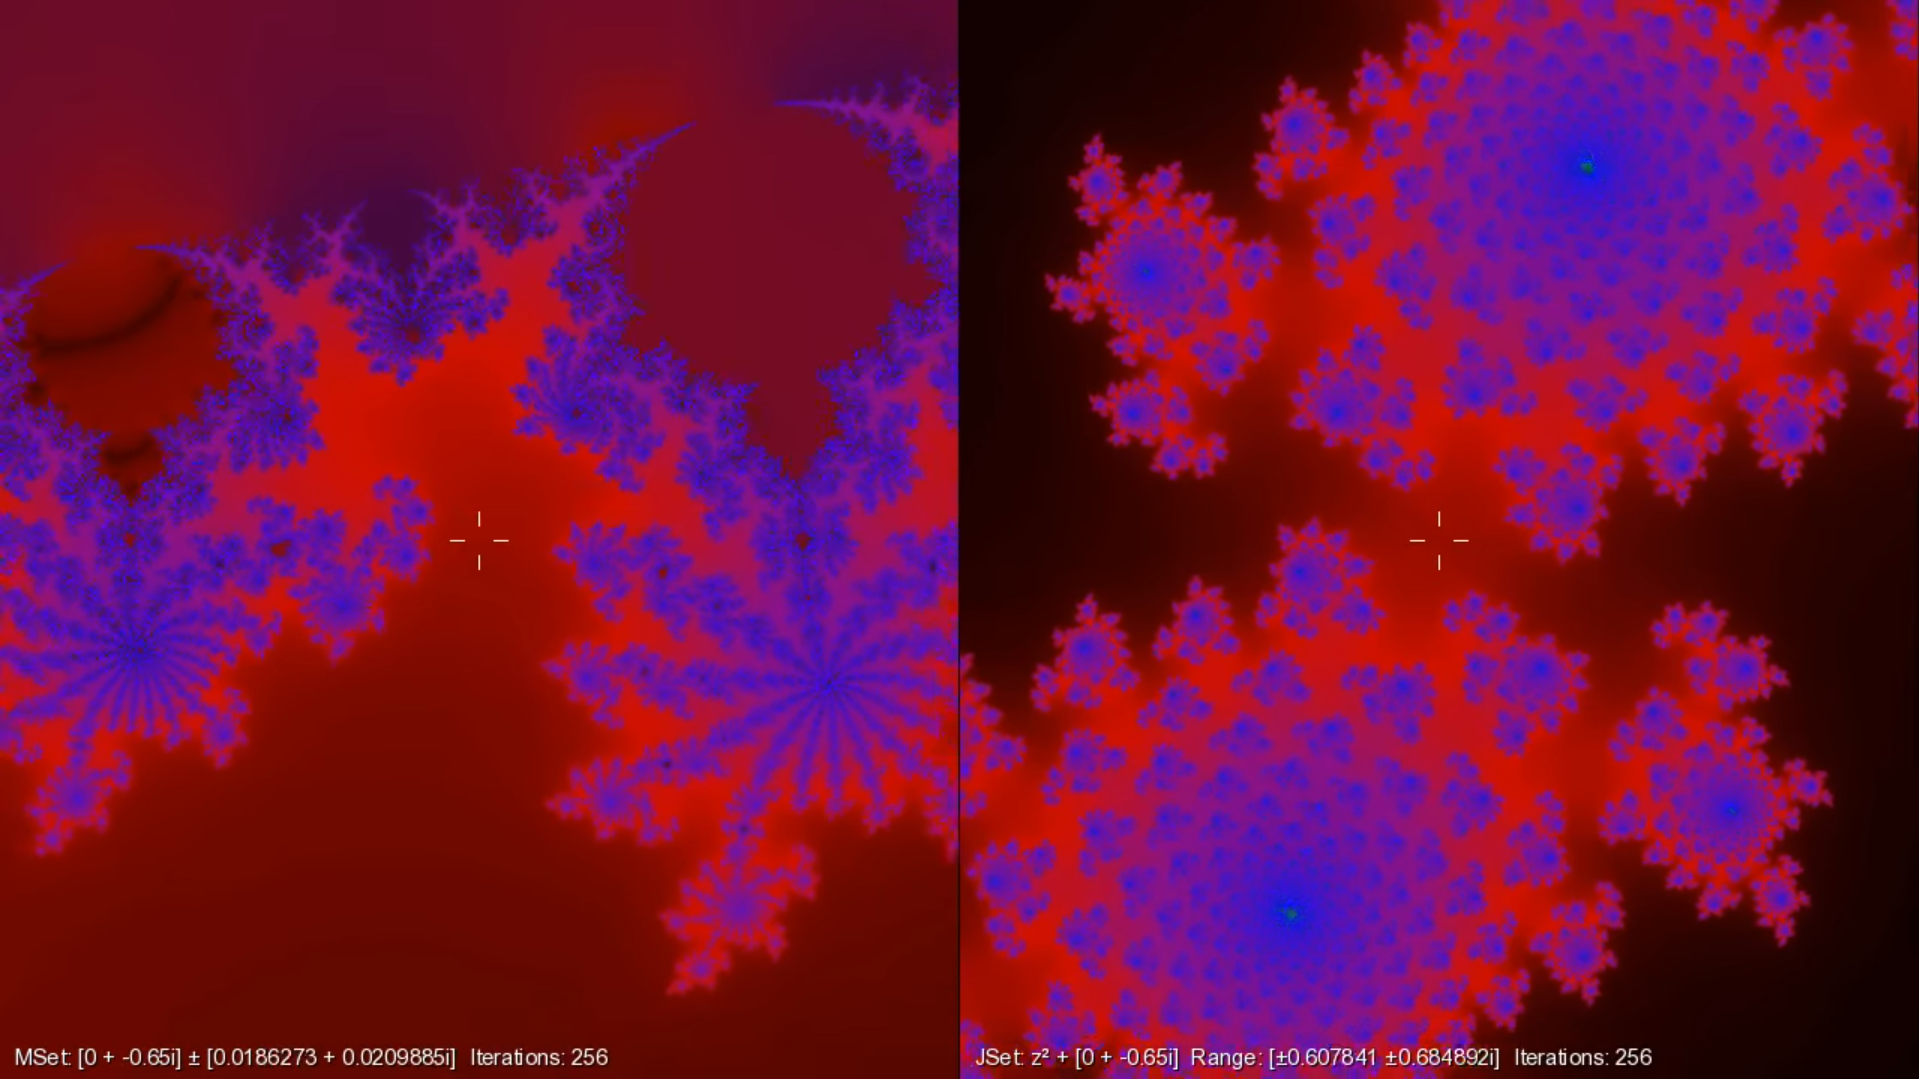
\includegraphics[width=\textwidth]{images/jmsets4.png}
    \caption[]{\label{fig:js2}MSet: $[0 + -0.65i]\pm[0.0186273+0.0209885i]$ Iterace: $256$.\\JSet: $z^2+[0 + 0.65i]$ Range: $[\pm0.607841 \pm0.684892i]$ Iterace: $256$.}
  \end{subfigure}
   
    \caption{ \label{fig:js3}Souvislost Mandelbrotovy množiny a Juliovy množiny.}
\end{figure}







% https://www.youtube.com/watch?v=fDSIRXmnVvk



% \subsection*{Bifurkace}

%
% \begin{figure}
%     \centering
%     \noindent
%     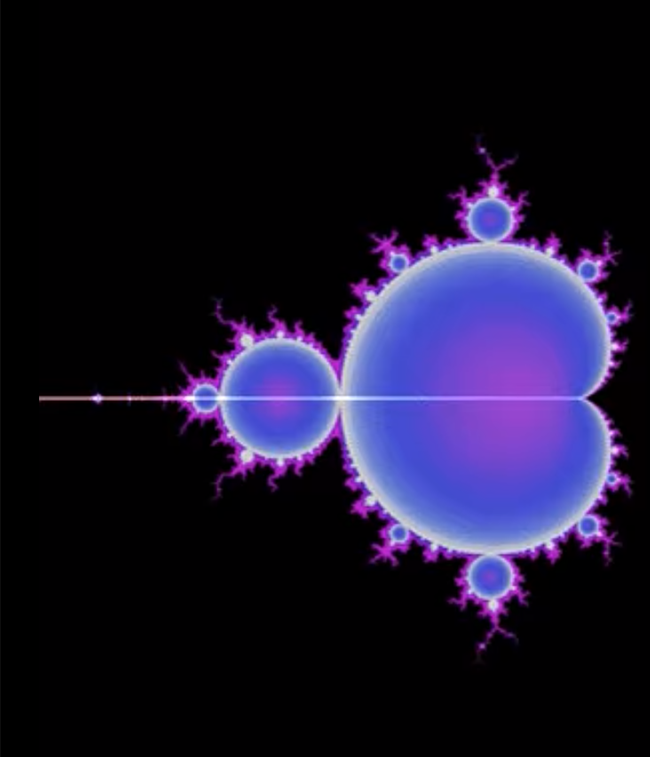
\includegraphics[width=0.45\textwidth]{images/hotentot1.png}\hspace{0.05\textwidth}%
%     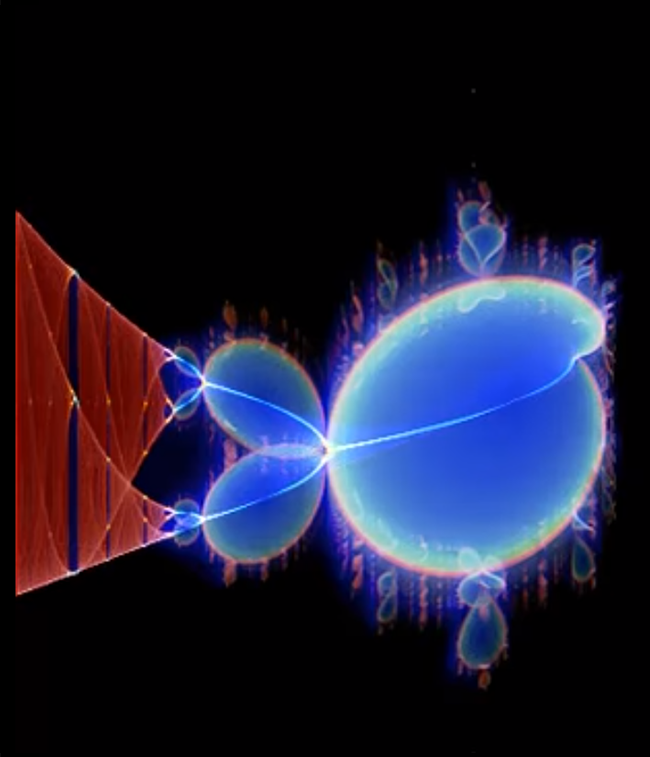
\includegraphics[width=0.45\textwidth]{images/hotentot2.png}\\[1em]
%     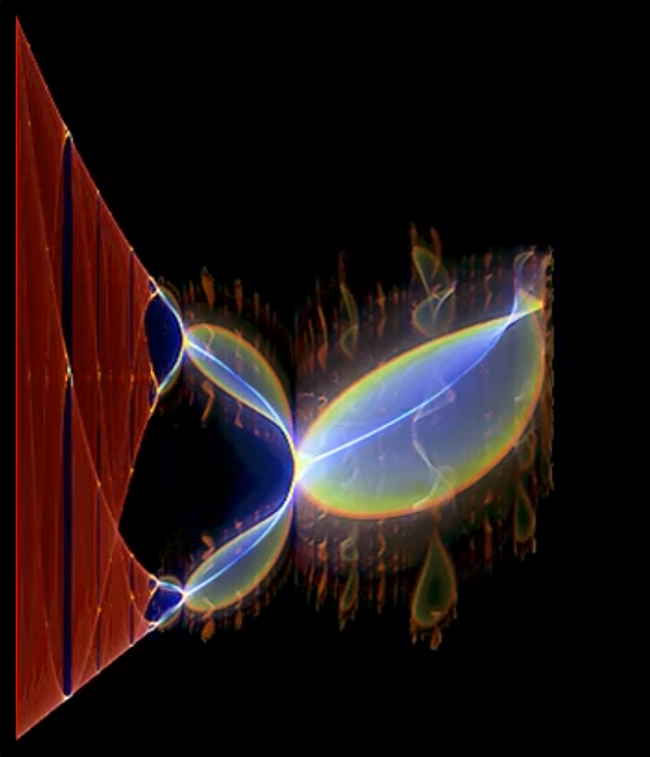
\includegraphics[width=0.45\textwidth]{images/hotentot3.png}\hspace{0.05\textwidth}%
%     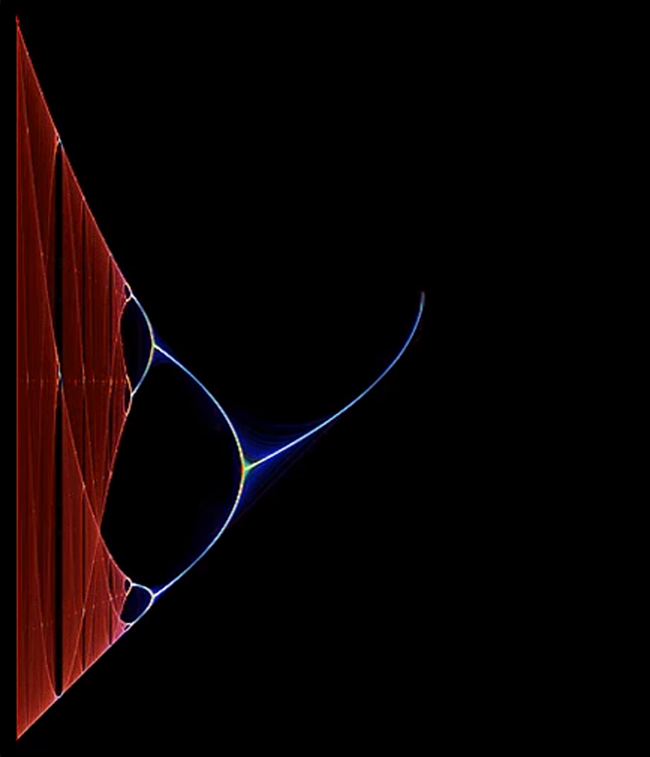
\includegraphics[width=0.45\textwidth]{images/hotentot4.png}\par
%     \caption{Mandelbrot bifurcation}
%     \label{fig:mandelbrot}
% \end{figure}

% \section{Escape-time fractals}


% use a formula or recurrence relation at each point in a space (such as the complex plane); usually quasi-self-similar; also known as "orbit" fractals; e.g., the Mandelbrot set, Julia set, Burning Ship fractal, Nova fractal and Lyapunov fractal. The 2d vector fields that are generated by one or two iterations of escape-time formulae also give rise to a fractal form when points (or pixel data) are passed through this field repeatedly.


\newpage

\section{Náhodné fraktály}

Náhodné fraktály se vyznačují tím, že jsou generovány algoritmy, do nichž je vnesena náhoda. Tím ztrácejí na symetričnosti a lépe tak odrážejí přírodní jevy. Výsledná podoba je ovlivněna způsobem, jak byla náhoda do generování zakomponována. Výhodou přidání náhody je i získání alternativ stejného fraktálu. \figurename~\ref{fig:lsysRand}\footnote{Zdroj: \url{https://cs.wikipedia.org/wiki/L-systém}} je příkladem několika alternativ stromů pomocí randomizovaného úhlu otočení.

\begin{figure}[h]
    \centering
    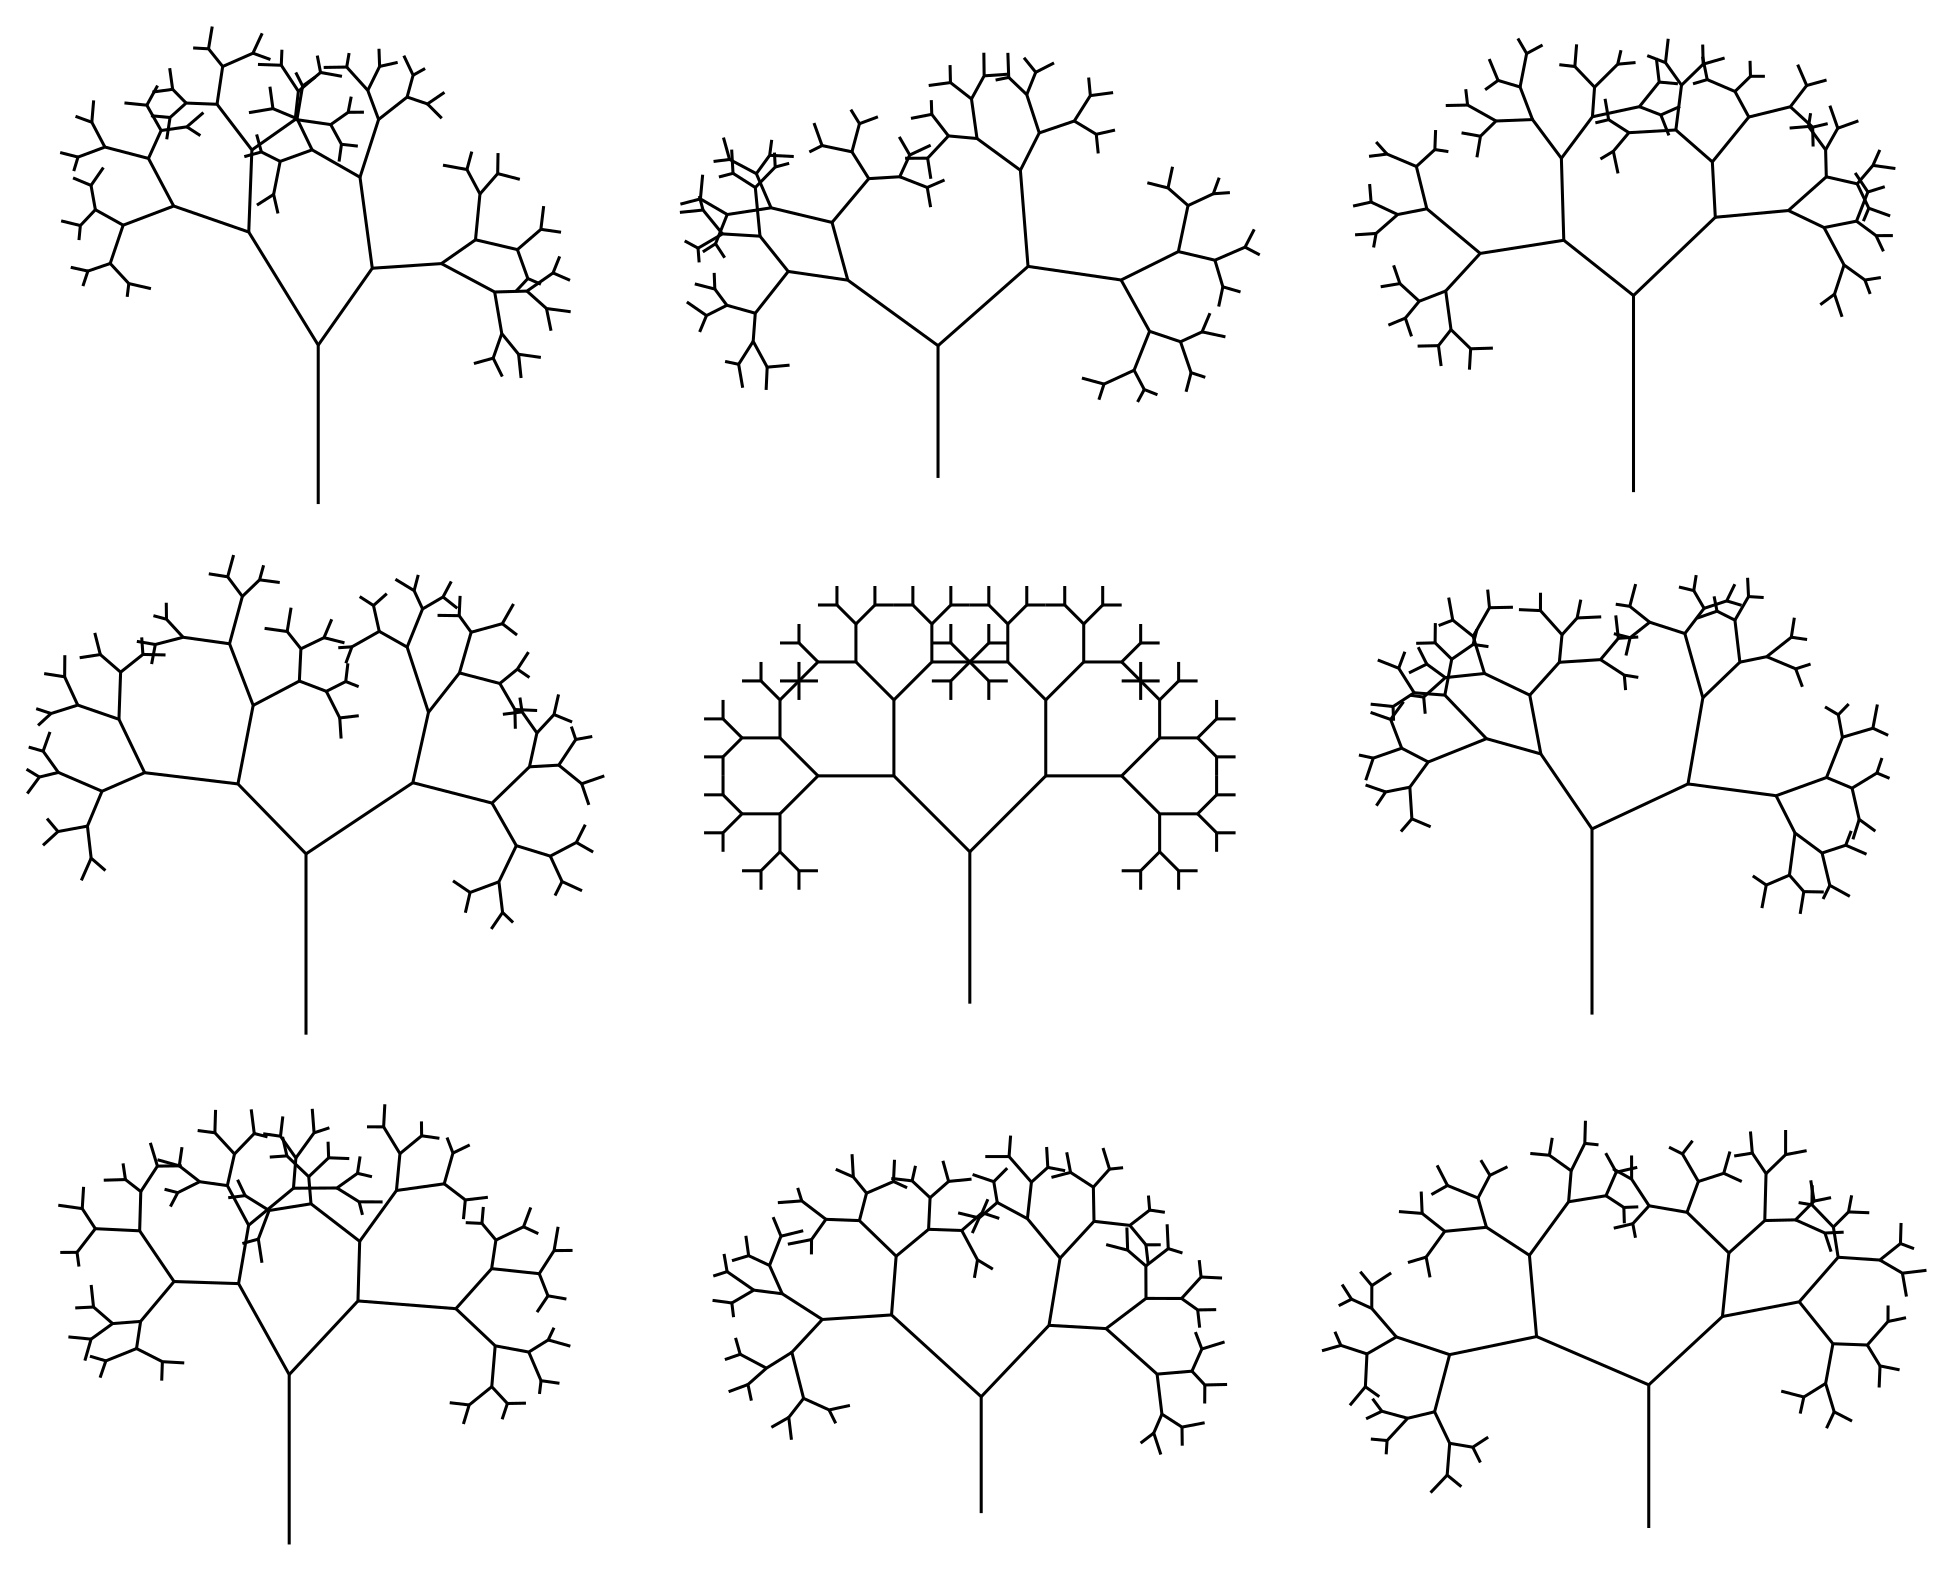
\includegraphics[width=300pt]{images/lsysRand.png}
        \caption{Stromy vygenerované pomocí L-systémů za použití randomizace.}
        \label{fig:lsysRand}
\end{figure}

\subsection*{Přírodní náhodné fraktály}

% https://cs.qwe.wiki/wiki/Diffusion-limited_aggregation


Fraktálem je i pobřeží (existuje i pojem "coastline paradox", neboli paradox pobřeží), neb má vlastnosti fraktální křivky, jejíž délka závisí na měřítku. Při přiblížení je možné naměřit délku navýšenou o struktury odhalené novým měřítkem. Pobřeží a obecně terén lze generovat pomocí počítačové grafiky, za využití například různých šumů, generátorů náhodných čísel a interpolace. Generováním fraktálního terénu se například věnuje práce \cite{kriz2019} z roku 2019. Mezi příklady náhodných fraktálů tedy patří:

\newpage

\begin{itemize}
  \item Brownův pohyb,
  \item \textit{Lévy flight} (Lévyho let - alternativa náhodné procházky),
  \item \textit{percolation clusters} (perkolační klastry),
  \item \textit{self avoiding walks} ("sobě se vyhýbající cesty"),
  \item fraktální krajiny,
  \item trajektorie Brownova pohybu a \textit{Brownian tree} (Brownovský strom), či
  \item dendritické fraktály modelovány agregací s omezenou difúzí (DLA).
\end{itemize}

Příklad fraktálu, který vznikl procesem difúzní limitní agregace zobrazuje \figurename~\ref{fig:dla}\footnote{Zdroj: \url{https://www.researchgate.net/figure/Distribution-of-particles-determined-by-a-diffusion-limited-aggregation-DLA-process_fig3_224053708}}

\begin{figure}[h]
    \centering
    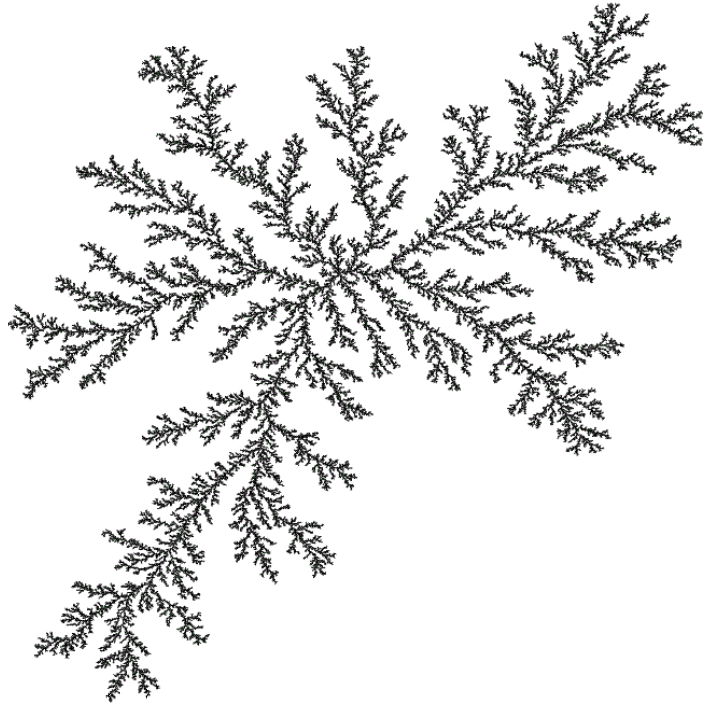
\includegraphics[width=260pt]{images/dla.png}
        \caption{Přírodní fraktál (proces difúzní limitní agregace).}
        \label{fig:dla}
\end{figure}


\note{V počítačové grafice je běžné vygenerovat vegetaci (například pomocí L-systémů) a rozpohybovat ji simulováním působení větru, atd.}

\newpage

% \section{Finite subdivision rules}

% Rekurzivní způsob rozdělování polygonu, nebo obecněji 2D útvaru na stále menší části.

% Metoda \textit{finite subdivision rules} dokáže popsat například \textbf{Penroseovo dláždění}.

% \textit{Barycentric subdivision}, neboli rozdělování z těžiště je příklad takového konečného rozdělovacího pravidla.

% Příkladem mimo počítačovou grafiku může být i \textit{teselace}, neboli plnění roviny pomocí jednoho nebo více geometrických útvarů bez překrývání a bez mezer. Často jde o různé vzory použité v keramických obkladech, například islámský dekorativní \textit{girih}, nebo díla nizozemského umělce M. C. Eschera.

% \begin{figure}[htbp]
%     \centering
%     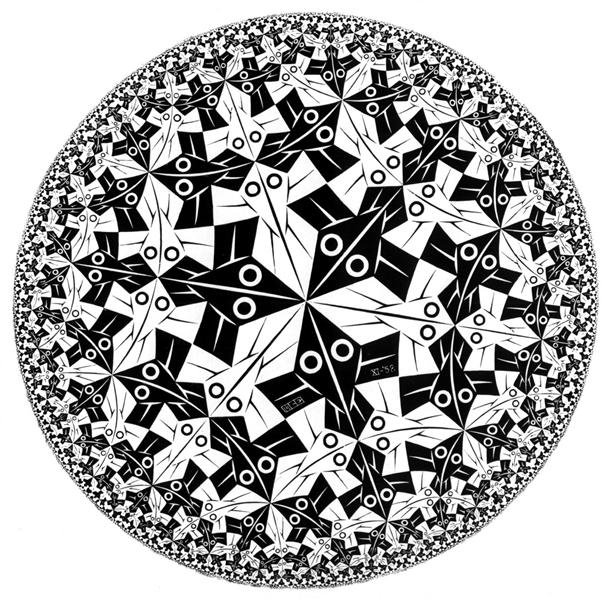
\includegraphics[width=200pt]{images/circle-limit.jpg}
%         \caption{Maurits Cornelis Escher - Circle limit I.}
%         \label{fig:escher}
% \end{figure}


% use a recursive topological algorithm for refining tilings[48] and they are similar to the process of cell division.[49] The iterative processes used in creating the Cantor set and the Sierpinski carpet are examples of finite subdivision rules, as is barycentric subdivision.



\section{Cohomology fractals}


\textit{Cohomology fractals}\footnote{Jde o práci z roku 2020 uvedenou zde spíše pro zajímavost.} popsali David Bachman, Saul Schleimer a Henry Segerman.  Jde o fraktály, tvořené různými 3D hyperbolickými varietami. \figurename~\ref{fig:coho}\footnote{Zdroj: \url{https://henryseg.github.io/cohomology_fractals/}} ilustruje pár možností nastavení parametrů.


\begin{figure}[h]
\centering
  \begin{subfigure}[b]{0.45\textwidth}
    
\includegraphics[width=\textwidth]{images/cohhom1.png}
    \caption[]{\label{fig:coho1}Fraktál v pohledovém módu vzdálenost.}
  \end{subfigure}
  \begin{subfigure}[b]{0.45\textwidth}
    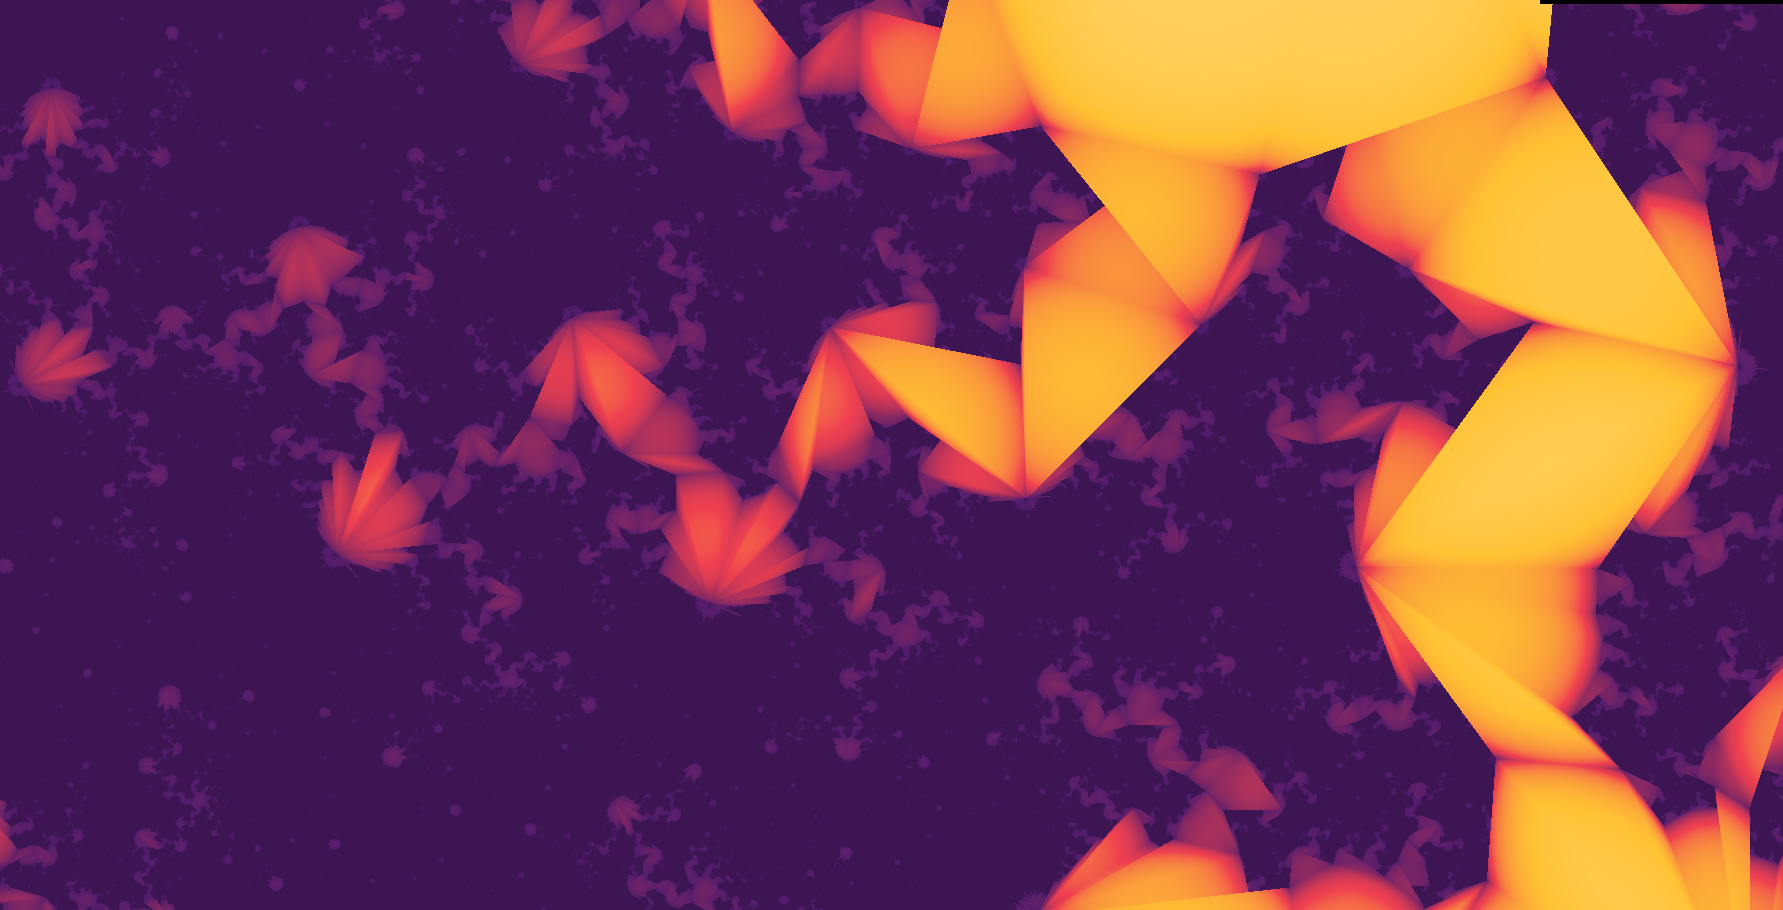
\includegraphics[width=\textwidth]{images/cohhom2.png}
    \caption[]{\label{fig:coho2}Fraktál pomocí jiné variety v pohledovém módu cohomology.}
  \end{subfigure}
   
    \caption{ \label{fig:coho}Cohomology fraktály.}
\end{figure}

% \begin{figure}
%     \centering
%     \noindent
%     
\includegraphics[width=0.45\textwidth]{images/1.jpg}\hspace{0.05\textwidth}%
%     
\includegraphics[width=0.45\textwidth]{images/2.jpg}\\[1em]
%     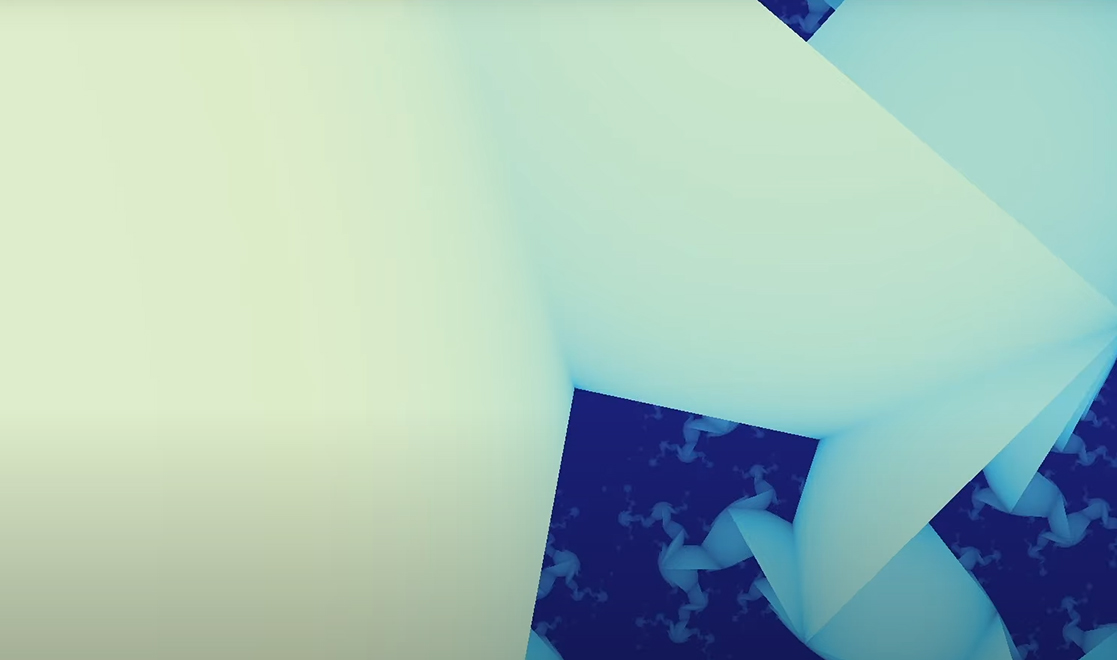
\includegraphics[width=0.45\textwidth]{images/3.jpg}\hspace{0.05\textwidth}%
%     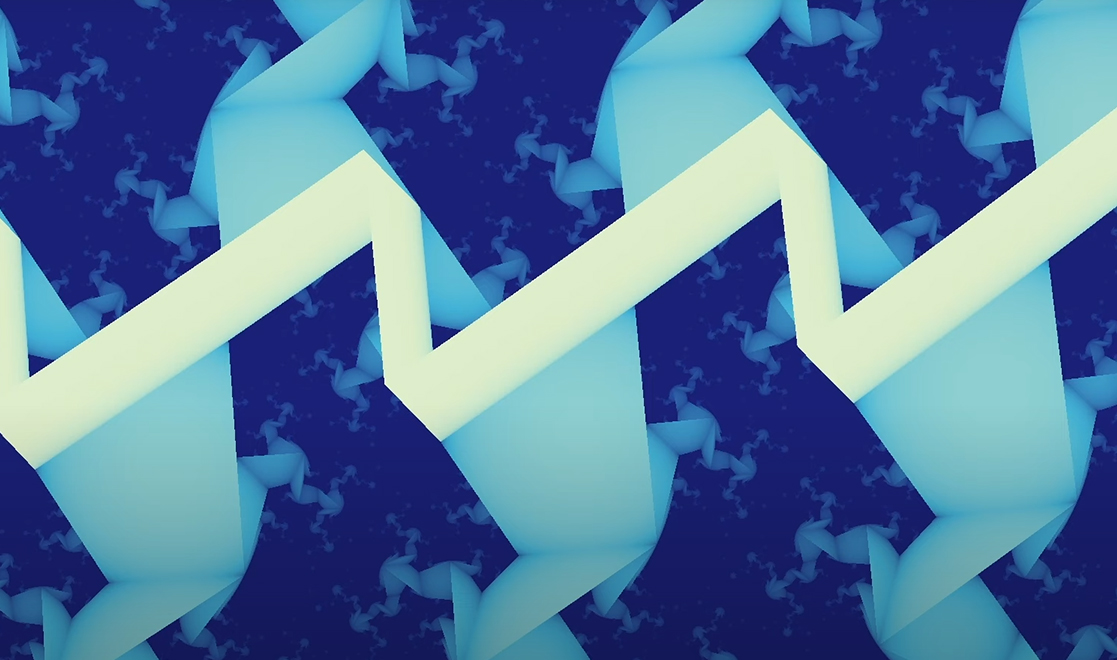
\includegraphics[width=0.45\textwidth]{images/4.jpg}\\[1em]
%     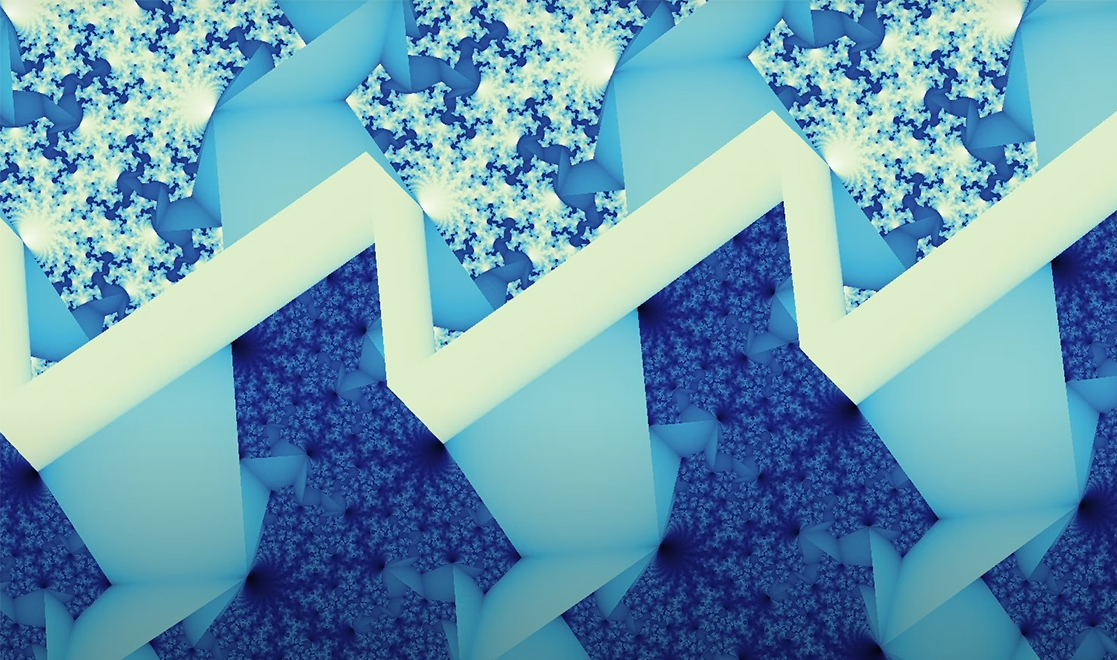
\includegraphics[width=0.45\textwidth]{images/5.jpg}\hspace{0.05\textwidth}%
%     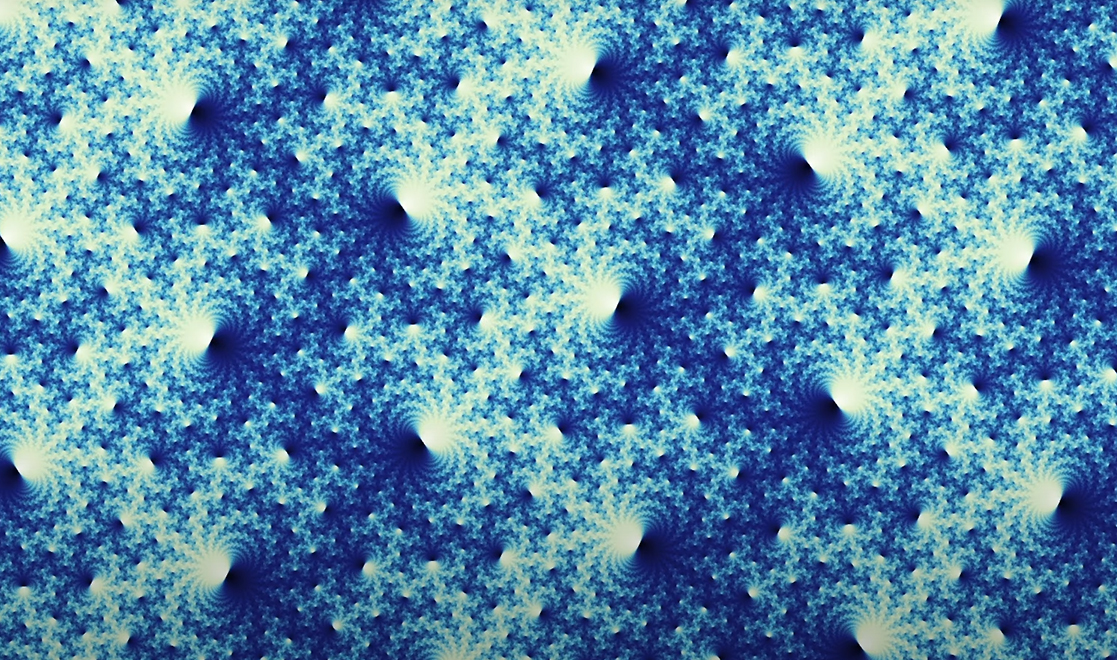
\includegraphics[width=0.45\textwidth]{images/6.jpg}\par
%     \caption{Postup konstrukce \textit{Cohomology fractals}}
%     \label{fig:cohomology}
% \end{figure}

% https://www.youtube.com/watch?v=fhBPhie1Tm0&feature=youtu.be


\begin{quote}[Cohomology fractals \cite{bachman2020cohomology}]{David Bachman}
"We introduce cohomology fractals; these are certain images associated to a cohomology class on a hyperbolic three-manifold. They include images made entirely from circles, and also images with no geometrically simple features. They are closely related to limit sets of kleinian groups, but have some key differences. As a consequence, we can zoom in almost any direction to arbitrary depth in real time. We present an implementation in the setting of ideal triangulations using ray-casting."
\end{quote}

\note{Jednoduchá "animace" \textit{cohomology} fraktálů by mohlo být přibližování a pohybování se v prostoru. Lze se domnívat, že dalších animací by šlo docílit jemnými přechody mezi definic variet.}

% --------------------------------------------------------- %
\newpage
\chapter{Příklady vizualizace hudby}

\begin{figure}[h]
    \centering
    \includegraphics[width=260pt]{images/rocketMan.png}
        \caption{Vizualizace skladby programu \textit{Windows Media Player}}
        \label{fig:mediaPlayer}
\end{figure}

Nápad vizualizovat hudbu zdaleka není novinkou. Existuje mnoho způsobů, jak toho docílit a proto bude výběr v této kapitole specifikován na netriviální způsoby. Těmi se pro účely této práce bude rozumět triviální zobrazení frekvenčního spektra. Příklad ukazuje \figurename~\ref{fig:mediaPlayer}\footnote{Zdroj: \url{https://www.windows-media-player.com/set-up-the-visualizations/}}.


\section{Vizualizace živé hudby}

Poptávka po vizualizacích k hudbě je žádaná při hudebních vystoupeních. Takové vizualizace by měly umět reagovat na právě hranou hudbu. To může mít na starost VJ (visual DJ) -- osoba zodpovědná za zobrazování vizualizací hodících se k hudbě v reálný čas. Další možností je vytvoření programu, který přizpůsobuje vizualizace hudbě. Tyto možnosti zkoumal již Vadim Petrov\cite{Petrov} ve své práci, kde vytvořil i vlastní aplikaci použitou ve svém vystoupení.

\begin{figure}
    \centering
    \includegraphics[width=300pt]{images/petrov.png}
        \caption{Živé představení Vadima Petrova}
        \label{fig:petrov}
\end{figure}


\section{Klasické vizualizéry hudby}

Za \emph{klasické vizualizéry hudby} jsou v této práci považovány programy přijímající jako vstup audio nahrávku, ke které v reálném čase generují doplňkové vizualizace.

\subsection*{Milkdrop 2.0}

\textit{Milkdrop} je \textit{plugin} programu na přehrávání hudby \textit{Winamp} vytvořený původně v roce 2001 Ryanem Geissem. Krása \textit{Milkdrop} spočívá v prolínavosti mezi neustále se měnícími vizuály, jak je ukázáno na obrázku \ref{fig:milkdrop}.

Podle dokumentace\cite{milkdrop} používá detekci rytmu, vyvolává nesčetné psychedelické efekty a vytváří bohatou vizuální cestu zvukem. \textit{MilkDrop} může pro vizualizace používat také živý vstup (mikrofon nebo line-in).

\begin{figure}
    \centering
    \noindent
    \includegraphics[width=0.45\textwidth]{images/winamp0.png}\hspace{0.05\textwidth}%
    \includegraphics[width=0.45\textwidth]{images/winamp1.png}\\[1em]
    \includegraphics[width=0.45\textwidth]{images/winamp2.png}\hspace{0.05\textwidth}%
    \includegraphics[width=0.45\textwidth]{images/winamp3.png}\par
    \caption{Plugin \textit{Milkdrop 2.0} pro program \textit{Winamp}}
    \label{fig:milkdrop}
\end{figure}


\subsection*{PySpace}
PySpace od CodeParade\cite{CodeParade} je hudební vizualizér. Je unikátní použitím rendereru \textit{Ray Marching} na vykreslování trojrozměrných fraktálů. Touto technikou je možné generovat fraktály v reálném čase a relativně lehce získat měkké stíny, \textit{ambient occlusion}, nebo dokonce kolize\footnote{Příklad ve videu: \url{youtu.be/9U0XVdvQwAI}}. Ukázka PySpace je k vidění na obrázku \ref{fig:pyspace}\footnote{Zdroj: \url{youtu.be/EkZsPcsV7yE}}.

% Distance Estimated 3D Fractals\\*
%  Je ve 4K\\*

\begin{figure}
    \centering
    \includegraphics[width=350pt]{images/3d_fractals.png}
    \caption{\label{fig:pyspace}Hudební vizualizér \textit{PySpace}}
\end{figure}

\pagebreak

\subsection*{Friktal}

Projekt \textit{Friktal}, mimo jiné i s aktivní komunitu na komunikační platformě \textit{Discord}, opět využívá trojrozměrné fraktály k vizualizaci. Uživatel prochází surrealistickým světem, který reaguje na hudbu. Projekt je k červenci roku 2020 stále ve vývoji.

Aplikace je interaktivní. Do vizuální projekce je možné použít i vstup z webové kamery v reálném čase a přispívat tak do vizuální produkce. Uživatel tak může například vidět svou tvář v kaleidoskopických fraktálovitých útvarech.

\figurename~\ref{fig:friktal}\footnote{Zdroj: \url{https://www.youtube.com/channel/UC66ZIkuYlxspf8NnmorFxqg}} je koláží ukázky z programu Friktal. V horních obrázcích byla použita interakce webkamery do vizualizací, obrázek vlevo dole znázorňuje navíc i živý vstup hraní na kytaru zachycený na mikrofon. Obrázek vpravo dole je klasický vstup z audio souboru bez webkamery.

\begin{figure}
    \centering
    \noindent
    \includegraphics[width=0.45\textwidth]{images/friktal0.png}\hspace{0.05\textwidth}%
    \includegraphics[width=0.45\textwidth]{images/friktal1.png}\\[1em]
    \includegraphics[width=0.45\textwidth]{images/friktal2.png}\hspace{0.05\textwidth}%
    \includegraphics[width=0.45\textwidth]{images/friktal3.png}\par
    \caption{Ukázka hudební vizualizace programu \textit{Friktal}.}
    \label{fig:friktal}
\end{figure}



%  https://friktal.com

\section{Souběžné generování hudby a vizualizací}

Tato sekce představí projekty, ve kterých je hudba s vizualizacemi úzce spjata. Jedná se o způsoby vytváření hudby zároveň poskytující obrazovou interpretaci procesu (\textit{Reactable}, \textit{SuperCollider}), či prakticky dokonalou vizualizaci hudby (\textit{Animusic}, \textit{Oscilloscope music}).

% Existují způsoby hudební produkce, mající za vedlejší efekt vizualizaci a vizualizace, které zároveň produkují hudbu. Tyto případy úzké provázanosti hudby a vizuální reprezentaci jsou zpravidla srozumitelné pro subjektivní interpretaci.

\subsection*{Reactable}

Reactable\cite{reactable} je elektronický hudební nástroj s fyzickým uživatelským rozhraním. Byl vyvinut \textit{Music Technology Group} na univerzitě v Barceloně. Projekt byl zahájen roku 2003 s cílem vyvinout nejlepší počítačový hudební nástroj nevázaný na konkrétní technologii.

Projekt ReacTable je jedním z možných použití \textit{tangible user interface} (TUI), neboli hmatatelným uživatelským rozhraním, jako nástroj kterým uživatel interaguje s digitální informací skrz fyzické prostředí. Jedním z průkopníků \textit{TUI} je Hiroshi Ishii, profesor Media Laboratory na MIT\footnote{Massachusetts Institute of Technology}. 

\begin{figure}[h]
\centering
\begin{minipage}{.5\textwidth}
  \centering
  \includegraphics[width=0.9\linewidth]{images/reactable.jpg}
  \captionof{figure}{Eletronický hudební nástroj \textit{Reactable}.}
  \label{fig:reactable}
\end{minipage}%
\begin{minipage}{.5\textwidth}
  \centering
  \includegraphics[width=0.9\linewidth]{images/sonicpi.png}
  \captionof{figure}{Živé vystoupení pomocí nástroje \textit{Sonic Pi}.}
  \label{fig:collider}
\end{minipage}
\end{figure}




% https://en.wikipedia.org/wiki/Tangible_user_interface



% \begin{figure}[h]
%     \centering
%     \includegraphics[width=230pt]{images/reactable.jpg}
%     \caption[]{\label{fig:reactable}Reactable}
% \end{figure}


% https://www.upf.edu/web/mtg/reactable

% http://www.nerdgen.net/2010/03/04/reactable-une-table-lumineuse-musicale.html

\subsection*{SuperCollider}
% https://www.youtube.com/watch?v=xXNB1BbKY8A

\textit{SuperCollider} je platforma pro syntézu zvuku a algoritmickou kompozici. Je používán hudebníky, umělci a ve výzkumu zvuku. Může být použit pro živé programování hudby. \figurename~\ref{fig:collider}\footnote{Zdroj: \url{youtu.be/G1m0aX9Lpts}} ukazuje použití programu podobného typu jako nástroje při živém vystoupení.

% https://supercollider.github.io

% \begin{figure}[]
%     \centering
%     \includegraphics[width=350pt]{images/super4.png}
%     \caption{\label{fig:collider}Živé vystoupení pomocí nástroje \textit{Sonic Pi}.}
% \end{figure}

\newpage

\section{Oscilloscope Music}

% Stranka ke se s tim da hrat => https://academo.org/demos/vectorscope/

Myšlenka za \textit{oscilloscope music}\footnote{Hudba používající osciloskop.} je vytvořit audiovizuální zážitek s úzkou korelací mezi obrazem a zvukem. Vizuály jsou proto vytvářeny stejnými zvukovými vlnami, jako hudba.

Pomocí osciloskopu lze měřit a vykreslovat časový průběh měřeného napěťového signálu. V případě \textit{oscilloscope music} je použit vektroskop, který umožňuje zobrazovat dva signály proti sobě na vertikální a horizontální ose. Vykreslován je zde levý a pravý audiokanál.

Tak by se dalo popsat nastavení, ve kterém lidé, věnující se \textit{oscilloscope music} zobrazují jejich hudbu. Jakákoliv hudba může být na osciloskop vykreslena, klíčem umělců jako Jerobeam Fenderson je většinou vymodelovat pomocí hudby konkrétní animované scény.

% \todo[fancyline]{tohle jeste poladit, hlavne posledni odstavec. dotaz - jdou skutecne smer hudba = > obraz  nebo spis neopak?}

% oscilloscope art

% Oscilloscope music - music that looks good when displayed on oscilloscope

% The idea behind that is to create audiovisual experience with closest possibel correlation between image and sound. Visuals are created from the exact same waveforms that you hear at the same time 

% oscilloscope is a piece of electrical testing equipement
% it does only one thing - it measures voltages and displays them on the screen

%there are several types of oscilloscopes - digital, analog

%he set it to x-y mode
%abd added second channel

% Magická kreslící tabulka Grafo (nebo jen Grafo) 

%difference to oscilloscope art - it is more about audio visual experience - images are drawn with the same waveforms that person hears 

% any music can be played on oscilloscope, the goal of many including Jerobeam Fenderson is to create music with interesting visual interpretation on oscilloscope

% https://oscilloscopemusic.com/tech.php

\begin{figure}
    \centering
    \noindent
    \includegraphics[width=0.45\textwidth]{images/osc1.png}\hspace{0.05\textwidth}%
    \includegraphics[width=0.45\textwidth]{images/osc2.png}\\[1em]
    \includegraphics[width=0.45\textwidth]{images/osc4.png}\hspace{0.05\textwidth}%
    \includegraphics[width=0.45\textwidth]{images/osc5.png}\par
    \caption[\textit{Oscilloscope music}]{\label{fig:oscilloscope}Oscilloscope music}
\end{figure}

% https://www.youtube.com/watch?v=B5ftW9GJff8
% https://www.youtube.com/watch?v=rtR63-ecUNo

\section{Animusic}

\textit{Animusic} je americká společnost založena roku 1995 specializujíc se na 3D vizualizace hudby. Společnost je známá pro počítačem generované animace, které vycházejí z \gls{midi} událostí, které mají vliv jak na hudbu, tak na vizuální efekty. Nástroje připomínají roboty hrající sami na sebe a animace se vyznačují dramaticky osvětlenými pokoji, nebo krajinou. V hudbě se nevyskytují vokály a většina zvuků je generovaná syntetizéry. \figurename~\ref{fig:animusic}\footnote{Zdroj: \url{https://www.animusic.com}} je příkladem takových animací.

% \begin{figure}[h]
%   \centering
%   \includegraphics[width=350pt]{images/animusic1.jpg}
%   \caption{Animusic}
%   \label{fig:animusic}
% \end{figure}

\begin{figure}[h]
\centering
  \begin{subfigure}[b]{1.0\textwidth}
    \includegraphics[width=\textwidth]{images/animusic1.jpg}
    % \caption[]{\label{fig:coho1}Fraktál v pohledovém módu vzdálenost.}
  \end{subfigure}\\
  \vspace{5pt}
  \begin{subfigure}[b]{1.0\textwidth}
    \includegraphics[width=\textwidth]{images/animusic2.jpg}
    % \caption[]{\label{fig:coho2}Fraktál pomocí jiné variety v pohledovém módu cohomology.}
  \end{subfigure}
   
    \caption{ \label{fig:animusic}Animusic}
\end{figure}



% --------------------------------------------------------- %

% ========================================================= %
\part{Realizace}

\chapter{Rozbor možností implementace}

Při rozhodování který konkrétní přístup použít k implementaci, byla provedena následující úvaha výhod a nevýhod z užšího výběru možností.\footnote{Již ze zadání se uvažují pouze možnosti audio nahrávky, nikoliv živého vstupu.}

\section{Možnosti analýzy audio souboru}

V teoretické části práci byly představeny některé možnosti přístupu k analýze hudební nahrávce. Jedním z nich je oddělit stopy vokálů a nástrojů (případně nástroje rozdělit na více typů), například pomocí formátu \textit{stem}. Dalším je pak použití reprezentace v \gls{midi} formátu. Další možností je vhodně tyto přístupy kombinovat.

\subsection*{Využití rozdělení kanálu}

Využitím rozdělení audia do více stop by se různé skupiny nástrojů izolovaly a získala by se tak nad nimi větší kontrola.

\begin{itemize}
    \item Výhody:
        \begin{itemize}
            \item Možnost vizualizovat odděleně vokály a doprovod. 
            \item Možnost rozlišit doprovod na bicí, basy, klavír a ostatní.
            \item Analýza a vizualizace takto oddělených stop by byla přesnější.
        \end{itemize}
    \item Nevýhody
        \begin{itemize}
            \item Delší implementační čas. Výsledná analýza by byla pravděpodobně podobná jako při sjednocených kanálech.
            \item Problematika získávání vstupu. Musí být provedena analýza dostupnosti skladeb ve formátu \textit{stem}.
            \item Získat oddělení stop pomocí softwaru (například \textit{Spleeter}) není úplně přesné.
        \end{itemize}
\end{itemize}
\subsection*{Využití \gls{midi}}

Reprezentace pomocí \gls{midi} by rozhodně měla přijít v úvahu, jelikož jde o dokonalé vyjádření hudebních událostí.

\begin{itemize}
    \item Výhody
        \begin{itemize}
            \item Možnost vizualizovat přesné frekvence a konkrétní nástroje, které zvuky hrají.
            \item Možnost vizualizovat výstup z \gls{midi} zařízení v reálném čase na živé vystupování.
            \item K některým skladbám existuje jejich dostupná \gls{midi} reprezentace.
        \end{itemize}
    \item Nevýhody
        \begin{itemize}
            \item Problematika získávání \gls{midi} - ne vše lze získat, reprezentace není pro všechny.
            \item Pro automatickou konverzi získání \gls{midi} reprezentace je vhodnější mít oddělené stopy všech nástrojů a všech hlasů
%  https://www.youtube.com/watch?v=tffLG4i4wjU
        \end{itemize}
\end{itemize}


\section{Spotify API}

Možnosti \textit{Spotify \gls{api}} byly diskutovány v sekci \ref{spotify}. Jiné existující \gls{api} v této práci není uvedeno, jelikož byla posuzována pouze \gls{api} služeb streamujících hudbu a to od Spotify\footnote{Vlastnící firmu \textit{The Echo Nest}, která se specializuje na vývoj v oblasti hudby.} se zdá být nejrozsáhlejší.

\begin{itemize}
    \item Výhody
        \begin{itemize}
            \item Jedná se o již existující řešení.
            \item Při integraci \textit{Spotify \gls{api}} se získá i objemná databáze skladeb.
            \item Jednoduchá možnost oddělení vizualizací a přehrávání tzn. zařízení pro vizualizaci a pro přehrávání nemusí být stejné a není třeba implementovat vlastní přehrávač. \textit{Spotify} umožňuje vybrat zařízení pro přehrávání a díky tomu je i jednoduché použití velké promítací stěny, která nemusí mít zapojeny reproduktory.
        \end{itemize}
    \item Nevýhody
        \begin{itemize}
            \item Pro přehrávání celých skladeb nutnost účtu \textit{Spotify}.
            \item Riziko nedostupnosti a změn \textit{Spotify} služeb.
        \end{itemize}
\end{itemize}


% \todo[]{taky by to melo byt "rozhodnuti", resp. nejaky dalsi komentar k tomu co se kdy kde pouzilo, ne moc textu, ale alespon 1-2 odstavece by tu byt mely}

% \todo[]{on tu chybi navrh - minimalne bych sem vrazil nejaky wireframe, nebo rucne kresleny obrazek te klasicke verze "cesty z fraktalnich stromu" a k nemu opet popis. Aby bylo videt, jak se te verzi postupne priblizujete.}


\section{Závěr}

Bylo rozhodnuto pro využití \textit{Spotify \gls{api}}, která umožní soustředit se na grafickou stránku, poskytne databázi skladeb a jednoduchou možnost prezentování. Je zde rovněž možnost do budoucna změnit způsob získávání dat z hudby a benefitovat z existující implementace vizuálů a zkušeností s tím, na co se v implementaci vlastní analýzy zaměřit.

\figurename~\ref{fig:fravizVize} znázorňuje původní grafický návrh aplikace jako "surrealistické krajiny" s fraktály reagujícími na vizualizace. Byla zde i představa rozšíření do "galaxie planet", každá s jinými vizualizacemi hudby. Nad obzorem mělo vycházet a zapadat slunce (případně měsíc) podle časového postupu v hudbě. Vizí byla i trajektorie průletu po manifoldu a možnost při přetáčení skladby se vrátit na stejné místo ve vizualizacích.


\begin{figure}[h]
\centering
    \includegraphics[width=\textwidth]{images/fravizVize.png}
    \caption{ \label{fig:fravizVize}Počáteční návrh aplikace \textit{Fraviz}.}
\end{figure}



\chapter{Postupný vývoj prototypu}
\label{evolution}

V rámci této práce vznikalo množství verzí prototypů postupně se přibližující původní vizi. Některé z nich v této kapitole budou popsány, jakožto podklady pro nadcházející verze prototypů.

\section{Předchozí verze}

Za předchůdce nápadu vizualizace hudby pomocí fraktálů by se daly považovat velmi naivní \textit{pluginy} autorky této práce triviálně vizualizující frekvenční spektrum dané skladby na SAGE\footnote{Framework (aplikační rámec) umožňující účastníkům přístup, zobrazení a sdílení informací v řadě rozlišení a formátů z více zdrojů na telestěnách, zpravidla z více monitorů.} a jednoduchý generátor fraktálovitých objektů podle parametrů. 
% \figurename~\ref{fig:predecessors} obsahuje oba jednoduché pluginy.

\begin{figure}[h]
\centering
%   \begin{subfigure}[b]{0.45\textwidth}
%     \includegraphics[width=\textwidth]{images/previous_versions/00.png}
%     \caption{Plugin pro SAGE}
% % https://www.evl.uic.edu/datsoupi/420/docs/SAGE2intro.pdf
%     \label{fig:sage}
%   \end{subfigure}
%   %
%   \begin{subfigure}[b]{0.45\textwidth}
    \includegraphics[width=0.5\textwidth]{images/previous_versions/01.png}
    \caption{Plugin pro Blender}
    \label{fig:blender}
%   \end{subfigure}
   
    % \caption{ \label{fig:predecessors}Předchůdci nápadu vizualizace hudby pomocí fraktálů.}
\end{figure}

% https://gitlab.fit.cvut.cz/BI-PGA/stud/hoskorad/blob/master/semestralka_sage/Audio_Visualizer.js
% \begin{verze}
% {Přehrávač pro \textit{SAGE}}
% {0.1}
% {HTML + Web Audio API}
% {nahrávka ve formátu mp3}
% {images/previous_versions/00.png}
% {Prvotní verze pouze zobrazovala frekvenční\\ spektrum a časový postup skladbou.}
% \end{verze}


\subsection*{Verze využívající audio soubor}

Všechny prototypy byly navrženy pro webové rozhraní z důvodu jednoduchého nasazování softwaru pro přístup veřejnosti. Pro vizualizace byla použita\footnote{Kromě prvního pokusu jednoduché mřížky bez knihoven.} \textit{javascriptová} knihovna \textit{Threejs}. Ve všech případech animace mají evokovat průlet krajinou. K tomu slouží pohybující se mřížky směrem k pozorovateli. 

% \todo[]{jak? - reaguji na konkretni frekvence(?co to bylo?) hudby (lisi se dla barev objektu) svym zvetsenim, ci zmensenim} V prvotních verzích (zobrazených na obrázcích \ref{fig:firstVersions}) to byly jednoduché geometrické útvary, které se měly časem nahradit fraktály.

% \begin{verze}
% {První Threejs verze reagující na zvukový input}
% {1.2}
% {Threejs + Web Audio API}
% {změna kamery, výběr z pár přednastavených skladeb}
% {images/previous_versions/fraviz04.png}
% {Pro vizualizace byly prvně použity jednoduché \\
% mnohostěny rozdělené na tři skupiny podle barvy, které \\
% reagovaly na \textit{beaty} v hudbě. Největší a nejvzdálenější tmavě\\
% modrý mnohostěn reprezentoval \textit{beaty} basů, prostřední \\
% růžové objekty středy a přední bílé mnohostěny \textit{beaty} výšek.\\
% Souvislý tyrkysový pruh měnil svou tloušťku podle \\
% hlasitosti. Rovněž rychlost průletu byla závislá \\
% na hlasitosti skladby.}
% \end{verze}


% \begin{figure}
% \centering
%   \begin{subfigure}[b]{0.45\textwidth}
%     \includegraphics[width=\textwidth]{images/previous_versions/fraviz07.png}
%     \label{fig:prev2}
%   \end{subfigure}
%   \begin{subfigure}[b]{0.45\textwidth}
%     \includegraphics[width=\textwidth]{images/previous_versions/fraviz04.png}
%     \label{fig:prev1}
%   \end{subfigure}
%   %
   
%     \caption{ \label{fig:firstVersions}Prvotní verze využívající pro vizualizaci audio soubor.}
% \end{figure}





% \subsection*{Web \gls{api}}

% Jednou z uvažovaných variant možných využití technologií bylo \textit{Web \gls{api}}\footnote{Zde je příklad takových aplikací: \url{https://webaudio.github.io/demo-list/}.}, umožňující ovládat právě hranou skladbu a tím vytvářet její alternovanou verzi. Tím by tak vznikla vysoce interaktivní aplikace umožňující interagovat i s hudbou.
% Zásahem uživatele by bylo možné získat další vstup pro vizualizace - přímo prováděnou transformaci hudby. Byl prototypován triviální přehrávač umožňující ovládat směr hudby z levého, či pravého reproduktoru.

\begin{figure}
  \centering
  \includegraphics[width=0.85\textwidth]{images/previous_versions/fraviz055.png}
  \caption{Ukázka změny pohledu kamery}
  \label{fig:cameraPerspective}
\end{figure}

\subsection*{Spotify \gls{api}}

Problémem předchozích přístupů bylo získání skladeb pro přehrávání. Jedním z řešení se nabízelo dovolit nahrát uživateli soubor z počítače, či využít \gls{api} existujících služeb pro streamování hudby zdarma, jako je například služba \textit{Soundcloud}. Byla zvolena služba \textit{Spotify} umožňující navíc využít \gls{api} pro analýzu skladeb popsanou v sekci \ref{spotify} a zároveň dovolujíc se tak více zaměřit na samotné vizualizace. 

% \begin{verze}
% {Implementace spotify API}
% {2.0}
% {v 1.2 + Threejs, Spotify API, spotify-viz}
% {hlasitost, bary, beaty, segmenty, tatumy a sekce}
% {images/previous_versions/fraviz10.png}
% {Všechny intervaly jsou zobrazeny pomocí škálování koule \\
%  poměrem celkové délky intervalu ku uplynulé délce.\\
% Díky tomu je možné ze začátku intervalu sledovat \\
% puls, který postupem intervalu mizí. Jedná se předem \\
% o verzi pro testování dat získaných ze \textit{Spotify \gls{api}}.\\
% Vektor frekvencí aktuálního segmentu popisovaný \\
% v \ref{spotify} je zobrazen pomocí dvanácti sloupců.\\
% Tyto sloupce jsou zrcadlově otočeny proti sobě \\
% a mění se s příchodem nového segmentu.}
% \end{verze}


\begin{figure}[b]
\centering
    \includegraphics[width=0.6\textwidth]{images/previous_versions/fraviz088.png}
    \caption{Přiblížení verze 2.0}
    \label{fig:dvanula}
\end{figure}
\newpage

% \begin{figure}[h]
% \centering
%     \includegraphics[width=0.8\textwidth]{images/previous_versions/fraviz10.png}
%     \caption{ \label{fig:firstThreejs}První verze Threejs vizualizací pomocí \textit{Spotify \gls{api}}.}
% \end{figure}



% \figurename~\ref{fig:firstThreejs2} využívá interpolaci barev podle \textit{beatu} a tím tak mění barvu abstraktních obrazců. Ty se otáčejí a škálují podle segmentů, beatů a barů. Verze byla poměrně chaotická a brzy se přešlo na jiný druh vizuálů.

% \begin{figure}[h]
% \centering
%     \includegraphics[width=0.8\textwidth]{images/previous_versions/fraviz09.png}
%     \caption{ \label{fig:firstThreejs2}Abstraktní stromy animované do hudby.}
% \end{figure}

% \begin{verze}
% {Abstraktní stromy animované do hudby}
% {2.2}
% {v 2.0 + d3-interpolate}
% {v 2.0 + index baru a beatu}
% {images/previous_versions/fraviz09.png}
% {Tato verze využívá interpolaci barev podle \textit{beatu}\\
% a tím tak mění barvu abstraktních obrazců. Ty se otáčejí \\
% a škálují podle segmentů, beatů a barů. Verze byla poměrně\\
% chaotická a brzy se přešlo na jiný druh vizuálů.}
% \end{verze}



%%%%%%%%



\subsection*{Fraktálovité stromy}\label{fractalLikeTrees}

První serióznější verze používá pro vizualizace objekty, připomínající fraktálovité stromy. Tyto stromy mění svou barvu při změně \textit{baru} a kývají se ze strany na stranu. Směr animace kývání je určován podle parity indexu \textit{baru}\footnote{Což vede k nerovnoměrnému pohybu ze strany na stranu, který ke konci skladby někdy vedl k zamotání celého stromu. Strom se totiž pohyboval trochu jako rameno robota - měl složené rotace větví.}. Jedna strana stromů se pohybovala na pulsy \textit{beatů}, druhá na pulsy \textit{barů}. 

Verze opět využívá chromatický vektor frekvencí pro každý nový segment. V této verzi je ovšem statický a mění se jen pozice, či škála sloupců. Jejich umístění má za účel evokovat hory. Tyto hory mění svou barvu a způsob vykreslování s každou sekcí. Sloupce jsou konstantních rozměrů a mění se jen jejich pozice na ose \textit{y}, nebo se škálují na ose \textit{y}. V tom případě se ještě vizualizace mohou lišit způsobem zarovnání (na střed sloupce, nebo spodní stranu sloupce).

Ve vizualizaci jsou další drobné experimentální prvky. Jedním jsou dvě malé sférické objekty obíhající konstantní trajektorii a pulsující do rytmu (původně mělo jít o světla). Druhým jsou pulsující stromy na horizontu. Pulsuje (nastaví průhlednost na maximum a postupně ji opět ztrácejí na minimum) pokud je jistota (\textit{confidence}) určeného \textit{beatu} větší, než hodnota 0.5. Závěrem různě testovaných hodnot bylo zjištění, že míra sepnutí této animace na základě přesnosti nelze dobře zobecnit pro všechny skladby.

Byla využita třída pro zobrazování statistik výkonu aplikace z důvodu ladění a pro informování uživatele o stavu aplikace. Lze vidět počet snímků za sekundu (FPS), doba renderování jednoho obrazu (ms) a využití paměti (MB).



% \todo[color=green]{super, presne ten text tu ma byt. Idealne formatvan, ale hlavni je, aby tu byl :)}

% \todo[]{a taky se zvetsovaly a hybaly - jak} \todo[]{alternativou pak bylo prime zobrazeni z API ziskanych informaci o prubehu useku bar, beat... atp. jendoducho formou pulzujicich sfer, ktere se ukazaly pro uzivatele na zaklade testovani jako jendoduchy, jasny a srozumitelny (a ciste informativni) zpusob vizualizace techto parametru.}


% \begin{verze}
% {Fraktálovité stromy}
% {3.3}
% {v 2.2 + stats.module}
% {v 2.2 + index sekce, jistota odhadu beatu}
% {images/previous_versions/fraviz11.png}
% {Tyto stromy mění svou barvu při změně \textit{baru}\\
% a kývají se ze strany na stranu. Podrobnější textový\\
% popis lze nalézt v podsekci "Fraktálovité stromy".}
% \end{verze}



\begin{figure}
    \centering
    \noindent
    \includegraphics[width=0.45\textwidth]{images/previous_versions/fraviz13.png}\hspace{0.05\textwidth}%
    \includegraphics[width=0.45\textwidth]{images/previous_versions/fraviz12.png}\\[1em]
    \includegraphics[width=0.45\linewidth]{images/previous_versions/tr6.png}\hspace{0.05\textwidth}%
    \includegraphics[width=0.45\linewidth]{images/previous_versions/tr5.png}\par
    \caption{Vizualizace pomocí fraktálovitých stromů.}
    \label{fig:fractalTrees}
\end{figure}


\newpage


\subsection*{Využití shaderů} \label{subs:vs}

Využití klasických trojdimenzionálních objektů vyplněných souvislou barvou se neukázalo jako optimální řešení pro tvorbu fraktálů a účely této aplikace\footnote{Připadalo v úvahu generovat trojdimenzionální fraktály pomocí L-systémů.}. Z toho důvodu dosavadní materiály vystřídaly shadery\footnote{Počítačové programy upravující jednotlivé programovatelné části zobrazovacího řetězce grafické karty.}, umožňující větší kontrolu nad vizualizacemi.

Kochova vločka, nebo alespoň křivka se objevuje na všech následujících vizualizacích. Je generována pomocí kaleidoskopických IFS, způsobu generování fraktálů přehýbáním prostoru popsaným v sekci \ref{kaleidoscope}. Pozdější verze aplikují měnící se texturu a tím tak utváří dojem kaleidoskopu.

\begin{figure}[h]
\centering
    \includegraphics[width=0.6\textwidth]{images/previous_versions/shader02.png}
    \caption{ \label{fig:shader}Využití shaderů v aplikaci.}
\end{figure}
\section{Popis uživatelského rozhraní}

Pro výběr a ovládání skladeb se používá přehrávač aplikace Spotify. Aplikace Spotify může být spuštěna ve webovém prohlížeči, nebo ji lze stáhnout do jiného zařízení (tablet, mobil, počítač, atd.).

Dalším prvkem pro ovládání je skrytí, či zobrazení minimalistického uživatelského rozhraní, které se provádí mezerníkem. V uživatelském rozhraní je možné vidět již zmíněné statistiky výkonu aplikace společně s interpretem a názvem skladby.

Aplikace má administrátorské rozhraní, které je pro uživatele skryto. Jedná se o pomocné rozhraní pro umísťování objektů do scény a nastavování hranic pro vizualizace (například vlnová délka a amplituda mřížky). Toto rozhraní nebylo testováno.


\begin{figure}[h]
\centering
    \includegraphics[width=0.4\textwidth]{images/previous_versions/stats.png}
    \caption{ \label{fig:shader}Statistiky výkonu aplikace.}
\end{figure}

\clearpage

% \begin{verze}
% {Bubliny}
% {2.2}
% {threejs + Spotify API}
% {spektum + volume, tatum, segment, beat, bar, section}
% {images/previous_versions/fraviz10.png}
% {tady muze byt \\ hafo textu o verzi}
% \end{verze}

%\section{Přehled klíčových verzí aplikace}

\begin{verze}
{Přehrávač pro \textit{SAGE}}
{0.1}
{HTML + Web Audio API}
{nahrávka ve formátu mp3}
{images/previous_versions/00.png}
{Prvotní verze pouze zobrazovala frekvenční\\ spektrum a časový postup skladbou.}
\end{verze}


\begin{verze}
{První Threejs verze reagující na zvukový input}
{1.2}
{Threejs + Web Audio API}
{změna kamery, výběr z pár přednastavených skladeb}
{images/previous_versions/fraviz04.png}
{Pro vizualizace byly prvně použity jednoduché \\
mnohostěny rozdělené na tři skupiny podle barvy, které \\
reagovaly na \textit{beaty} v hudbě. Největší a nejvzdálenější tmavě\\
modrý mnohostěn reprezentoval \textit{beaty} basů, prostřední \\
růžové objekty středy a přední bílé mnohostěny \textit{beaty} výšek.\\
Souvislý tyrkysový pruh měnil svou tloušťku podle \\
hlasitosti. Rovněž rychlost průletu byla závislá \\
na hlasitosti skladby.}
\end{verze}

\begin{verze}
{Implementace spotify API}
{2.0}
{v 1.2 + Threejs, Spotify API, spotify-viz}
{hlasitost, bary, beaty, segmenty, tatumy a sekce}
{images/previous_versions/fraviz10.png}
{Všechny intervaly jsou zobrazeny pomocí škálování koule \\
 poměrem celkové délky intervalu ku uplynulé délce.\\
Díky tomu je možné ze začátku intervalu sledovat \\
puls, který postupem intervalu mizí. Jedná se předem \\
o verzi pro testování dat získaných ze \textit{Spotify \gls{api}}.\\
Vektor frekvencí aktuálního segmentu popisovaný \\
v \ref{spotify} je zobrazen pomocí dvanácti sloupců.\\
Tyto sloupce jsou zrcadlově otočeny proti sobě \\
a mění se s příchodem nového segmentu.}
\end{verze}


\begin{verze}
{Abstraktní stromy animované do hudby}
{2.2}
{v 2.0 + d3-interpolate}
{v 2.0 + index baru a beatu}
{images/previous_versions/fraviz09.png}
{Tato verze využívá interpolaci barev podle \textit{beatu}\\
a tím tak mění barvu abstraktních obrazců. Ty se otáčejí \\
a škálují podle segmentů, beatů a barů. Verze byla poměrně\\
chaotická a brzy se přešlo na jiný druh vizuálů.}
\end{verze}

\clearpage

\begin{verze}
{Fraktálovité stromy}
{3.3}
{v 2.2 + stats.module}
{v 2.2 + index sekce, jistota odhadu beatu}
{images/previous_versions/fraviz11.png}
{Tyto stromy mění svou barvu při změně \textit{baru}\\
a kývají se ze strany na stranu. Podrobnější textový\\
popis lze nalézt v podsekci "Fraktálovité stromy".}
\end{verze}


\begin{verze}
{Kochovy tóniny}
{4.0}
{v 3.3 + GLSL shadery}
{v 3.3 + tonalita}
{images/previous_versions/fraviz16.png}
{Společně s vizuálním posunem, aplikace nyní umožňuje \\
přizpůsobit barevné schéma tonalitě skladby. Teplé barvy\\
jsou pro durovou tonalitu a studené pro mollovou tonalitu.\\
Barvy se opět střídají se změnou sekce.}
\end{verze}
    
\begin{verze}
{Taneční parket}
{4.1}
{v 4.0}
{v 4.0 + danceability}
{images/previous_versions/shader00.png}
{Nově přibyly vizualizace fraktálů generovaných pomocí\\
 L-Systémů, které se otáčejí s postupem času a od začátku\\
   taktu se rozpadají. Stromy po stranách navíc mizí\\
  v dáli. Zároveň byl zakomponován atribut danceability,\\
 který když je větší, než daná hodnota, objeví se povrch,\\
 který má simulovat taneční plochu. Skladba \\
splňující tuto hodnotu je například \textit{The Prodigy - Breathe}.}
\end{verze}
    
\begin{verze}
{Živé publikum}
{4.2}
{v 4.0}
{v 4.1 + liveness}
{images/previous_versions/shader08.png}
{Kaleidoskopická kochova vločka byla popsána v druhém \\
odstavci u "Využití shaderů". Dále u skladeb s parametrem\\
liveness větší, než je daná hodnota je více fraktálů\\
v popředí. Tím mají simulovat živé publikum. Jev lze vidět\\
na skladbě \textit{Traband - Viděl Jsem Člověka}.}
\end{verze}
    
    \clearpage
    
    
% \begin{figure}
% \centering
%   \begin{subfigure}[b]{0.45\textwidth}
%     \includegraphics[width=\textwidth]{images/previous_versions/fraviz16.png}
%     \caption{Mollová modalita.}
%     \label{fig:minor}
%   \end{subfigure}
%   %
%   \begin{subfigure}[b]{0.45\textwidth}
%     \includegraphics[width=\textwidth]{images/previous_versions/fraviz18.png}
%     \caption{Durová modalita.}
%     \label{fig:major}
%   \end{subfigure}
   
%     \caption{ \label{fig:shader}Vizualizace pomocí shaderů.}
% \end{figure}

%%%%%%%%%%%%%%%%%%%%%%



%%%%%%%%%%%%%%%%%%%%%%


% \todo[]{tady je moc hezkych obrazku a jsou moc male, resp. pokud pozdeji nekde budou ty finalnejsi verze ve vetsim, pak ok. k obrazkum 6.4 a 6,5 to chce vic popisne informace - co vsechno tam je a jak to reaguje...}

% \newpage

% \section{Detailnější popis Spotify API}

% Finální prototyp zakomponovává \textit{Spotify \gls{api}}. Pro vizualizace byly využity dva jeho koncové body, které byly popsány v teoretické části.

% \subsection*{Využití \textit{Get Audio Features for a Track}}

% Bližší vysvětlení atributů a jejich použití bude debatováno zde. Při interpretaci bylo vycházeno z přednášky\cite{spotifyLecture} o \textit{Spotify \gls{api} } a grafů v Příloze \ref{ch:C}.

% \paragraph{\textit{Acousticness}, \textit{speechiness}, a \textit{instrumentalness}}

% jsou atributy vhodné pro detekování absence zkoumaného jevu a původně byly zamýšleny jako binární klasifikátory. Lze díky tomu vyřadit skladby, které nejsou čistě akustické, skladby které určitě neobsahují převážně mluvené slovo\footnote{Což je velmi užitečné při automatizovaném přehrávání hudby pro vyřazení projevů, bonusových skladeb, atd.} a nebo skladby které s velkou pravděpodobností obsahují nějaké vokály.

% \paragraph{\textit{Danceability}, \textit{energy} a \textit{Tempo}}

%  se více přibližují normálnímu rozdělení a jsou proto vhodné pro vizualizace.





% \paragraph{Rekapitulační popis implementace atributů}

% \begin{itemize}
%     \item Barevné schéma podle modality. Teplé barvy pro durovou a studené pro mollovou.
%     \item Rychlost podle odhadovaného celkového tempa
%     \item Zvýšený úhel pohybu, pokud je skladba označena jako pravděpodobně vhodná pro tanec
%     \item Vyšší hodnoty energie pro více objektů ve scéně
% \end{itemize}

% \subsection*{Využití \textit{Audio Analysis Object}}

% \begin{itemize}
%     \item Sekce znázorňují jinou povahu či fázi hudby, proto vizualizace v různé sekce jsou navzájem odlišné
%     \item V každém segmentu se vizualizuje dominance jednotlivých tónů na chromatické stupnici
%     \item Zvlášť výrazné vizualizace, pokud je posuzovaný atribut odhadnut s velkou pravděpodobností
%     \item Návaznost beatů a barů
% \end{itemize}

% \subsection*{"Umělecký" záměr}

% Abstraktní fraktály jsou nejspíše vhodný pro co nejpřesnější hloubkové zobrazení všech hudebních nuancí a pro jemně plynulé přechody. Záměrem bylo ovšem vystavění scény, která bude připomínat průlet krajinou. Přidáním 3. rozměru by uživatel aplikace měl získat časový rámec a tedy představu toho, co bylo předtím a co potom. Celý zážitek by se měl dát připodobnit jízdě autem bez nutnosti ho řídit, krajinou, která se před očima proměňuje do rytmu hudby. Z toho důvodu byly zvoleny L-Systémy, jakožto jednoduché \textit{stromy}.



% \subsection*{Problém synchronizace}


% Aplikace při ovládání právě bežící skladby ztrácí synchronicitu a nefunguje definovaně.


% It seems that synchronization is not currently practical, because while the docs say that the "timestamp" field signifies when the API gave you the data, it actually does not do what it says because of some issue on their side: https://github.com/spotify/web-api/issues/1073

% Instead the timestamp seems to change only when there is a new song starting, pause, or seek. This means that as it is, we cannot know when the API response was generated.

%https://stackoverflow.com/questions/59029450/how-to-synchronize-clock-with-spotify-servers





% https://github.com/zachwinter/spotify-viz

% \begin{figure}[h]
% \centering
%     \includegraphics[width=0.4\textwidth]{images/previous_versions/stats.png}
%     \caption{ \label{fig:shader}Statistiky výkonu aplikace.}
% \end{figure}

% \section{Popis uživatelského rozhraní}

% Pro výběr a ovládání skladeb se používá přehrávač aplikace Spotify. Aplikace Spotify může být spuštěna ve webovém prohlížeči, nebo ji lze stáhnout do jiného zařízení (tablet, mobil, počítač, atd.).

% Dalším prvkem pro ovládání je skrytí, či zobrazení minimalistického uživatelského rozhraní, které se provádí mezerníkem. V uživatelském rozhraní je možné vidět již zmíněné statistiky výkonu aplikace společně s interpretem a názvem skladby.




\chapter{Použité technologie}

Pro lehký přístup přes internet byl prototyp napsán jako webová aplikace. V následující kapitole bude popsáno, jaké webové technologie byly použity. Finální prototyp používá \textit{Spotify \gls{api}} a pro usnadnění práce s touto službou je tento prototyp rozšířením existujícího repozitáře na stránce \textit{github.com}. Aplikace je napsaná v programovacím jazyce JavaScript.

% \section{Web Audio API}

% Web Audio API je specifikace vyvíjená W3C a popisuje JavaScriptové API pro zpracování a syntetizování zvuku ve webových aplikacích. Myšlenka spočívá ve vytvářání objektů, které definují produkci zvuku, dávajíc tak vývojářům možnost ve webových aplikacích zvuk upravovat i vytvářet. Je možné například přidávat více audio zdrojů najednou (což se hodí ve hrách), získávat data pro audio vizualizace, přidávání efektů do zvuku, nebo upravovat prostorové efekty (jako je přecházení z levého a pravého reproduktoru).

% source :  https://www.w3.org/TR/webaudio/


% Low-level JavaScript API based on the OpenGL ES 2.0 specification.

\section{Programovací a značkovací jazyky}

Ve stručnosti zde budou vyjmenovány programovací a značkovací jazyky pomocí kterých je napsán finální prototyp.

\paragraph*{HTML5}

je verze značkovacího jazyka \textit{\gls{html}} sloužícího pro tvorbu webových stránek. Proti předchozí verzi \textit{HTML4} z roku 1997 přináší podstatné změny, přičemž mezi nejdůležitější patří přímá podpora přehrávání multimédií v prohlížeči a podpora pro aplikace, které fungují i bez připojení k Internetu.

\paragraph*{Sass}
je preprocesorový a skriptovací jazyk \textit{syntactically awesome style sheets}, který je interpretován nebo kompilován do kaskádových stylů (\gls{css}) starajíc se o způsob zobrazení stránek psaných v \textit{HTML}. Oproti samotnému \gls{css} umožňuje psát kratší a přehlednější kód.


\paragraph*{JavaScript}

je multiplatformní, objektově orientovaný, \textit{event-driven} skriptovací jazyk. Odpovídá specifikaci \textit{ECMAScript}. Patří do skupiny vyšších programovacích jazyků a multiparadigmatických programovacích jazyků. Často využívá \textit{just-in-time} kompilaci.

\section{Vizualizace}

K vizualizacím se již od prvních verzí používala knihovna \textit{Three.js}, později se v \textit{Three.js} začalo využívat i shaderů.

\paragraph*{Three.js}

je JavaScriptová knihovna a aplikační rozhraní sloužící k vytváření a zobrazování 3D animací ve webovém prohlížeči. Využívá aplikační rozhraní \textit{WebGL}. \textit{Three.js} umožňuje do webové stránky začlenit 3D animace akcelerované přes grafický procesor (GPU). Knihovnu vytvořil Ricardo Cabello, aka Mr.Doob, a je na \textit{GitHubu} od roku 2010. Nyní je počet přispívajících uživatelů přes 1200.

% Three.js was created by Ricardo Cabello, aka Mr.Doob, and has been on gitHub since 2010. Since that time, it has received added help from many contributors and its user base has grown to a large size. Three.js provides several different draw modes and can fall back to the 2D rendering context if WebGL is not supported. Three.js is a well-designed library and fairly intuitive to use. Default settings reduce the amount of initial work or “boilerplate” needed. Settings can be overridden as parameters passed in upon object construction or by calling the appropriate object methods after \cite{Danchilla}.

\paragraph*{OpenGL Shading Language}

(zkráceně GLSL) je vyšší programovací jazyk pro psaní shaderů, který vychází ze syntaxe jazyka C pro všeobecné použití. Umožňuje ovládat programovatelnou část zobrazovacího řetězce.

\paragraph*{Knihovna d3-interpolate}

byla použita pro interpolaci číselných hodnot a barev. Díky \textit{d3-interpolate} je možné například zadat barevné spektrum dvěma barvami a získat tak postupné barevné přechody podle zadaných parametrů.

\section {Nasazení aplikace}

Byl použit repozitář zaštiťující \textit{back endovou} (serverovou) stránku aplikace a služba \textit{Heroku} pro nasazení.

\paragraph*{Repozitář \textit{spotify-viz}}

slouží jako základ aplikace. Je dostupný na stránce \textit{github.com} od uživatele \textit{zachwinter} zveřejněn s licencí MIT. Repozitář umožňuje autentizaci uživatele pomocí přesměrování na stránky služby \textit{Spotify} a tím tak začne poslouchat přehrávaná data z účtu přihlášeného uživatele. Repozitář má připravenou šablonu pro vizualizace. Výsledná stránka po přihlášení je pouze \textit{HTML} element \textit{canvas}, připravený na vykreslování dat z přehrávané hudby, která jsou obdržena pomocí dotazů (\textit{request}). Repozitář používá \textit{Node.js} framework \textit{Express.js} a balíčkovací správce (\textit{package manager}) \textit{npm}. Detailnější informace lze nalézt na stránce\cite{spotifyViz} projektu.


\paragraph*{Heroku}

je platforma umožňující rychlé nasazování webových aplikací. Původně podporovala pouze \textit{Ruby}, nyní podporuje jazyky \textit{Java}, \textit{Node.js}, \textit{Scala}, \textit{Clojure}, \textit{Python}, \textit{PHP} a \textit{Go}. Je ve vývoji od roku 2007, jako jedna z prvních cloudových platforem. Název je spojením slov "heroic" a "haiku".

Aplikace je dostupná na webové adrese: \url{http://fraviz.herokuapp.com}.


% \subsection*{Babylon.js}

% Realtime 3D engine používající JavaScript pro zobrazování 3D grafiky ve webovém prohlížeči, který využívá HTML5. Je napsán v programovacím jazyce TypeScript, jelikož umožňuje psaní dostatečně robustního kódu. TypeScript je dále transcompilován na JavaScript. Babylon.js 3D engine je nativně interpretován všemi prohlížeči podporující standard HTML5 a WebGL provádějící 3D rendering. 

% Babylon.js poskytuje možnost si na webu vyzkoušet interaktivní fragment a shader editor, sdílet výtvory a vygenerovat z poskládaných nodes javascriptový kód.

% \subsection*{WebGPU}

% WebGPU je název budoucího webového standartu a JavaScriptového API pro akceleraci grafiky. Projekt je vyvíjen \textit{W3C GPU for Web Community Group} s vývojáři z Apple, Mozilla, Microsoft, Google a dalšími. Technologie je stále ve vývoji a měla by nahradit WebGL.

% The promise behind WebGPU is an awesomely faster API providing lower level control to the graphic resources from Javascript.

%  https://github.com/BabylonJS/Documentation/blob/master/content/extensions/WebGPU/webGPU.md

% JavaScriptové frameworky jako Babylon.js již připravují podporu WebGPU.

% --------------------------------------------------------- %
\chapter{Testování}

Tato kapitola obsahuje závěry z průběžného uživatelského testování. Výsledky těchto poznatků byly podkladem pro soustavné zlepšování aplikace v rámci jednotlivých verzí. Primárně byly testovány verze 2.0 až 3.0. 

\section{Persony}

Byly vytvořeny dvě abstraktní persony pro uživatelské testování aktuálního stavu aplikace tak, aby reprezentovaly velkou část z celkové skupiny možných uživatelů.

\subsection*{Persona A: Student informatiky}

Persona studenta, jehož věk je zhruba 20 let. Na počítači tráví většinu svého času a rozumí informatice. Občas poslouchá hudbu a rád by také ji také produkoval.

\subsection*{Persona B: Nadšenkyně do hudby}

Persona ženy, které je zhruba 45 let se zájmem o hudbu. Počítač používá pouze uživatelsky a informatice se nevěnuje. Za to ráda poslouchá hudbu, zpívá a hraje na kytaru.

\subsection*{Persona C: Umělec}

Persona umělce, jemuž je zhruba 30 let a věnuje se výtvarnému umění. Věnuje se i počítačovým vizualizacím, tudíž si rozumí s počítačem.

\section{Scénáře testování}

Testování bylo rozděleno na dvě skupiny. První je ovladatelnost aplikace. Možnými úkony jsou přihlášení do aplikace a ovládání skladeb. Přihlašovací systém je formou přesměrování na stránku \textit{Spotify} a ovládání skladeb je formou \textit{Spotify} přehrávače. Testování této skupiny nebylo hodnoceno, jelikož využívá uživatelské rozhraní třetí strany (\textit{Spotify}). 

Druhou skupinou testování, bylo subjektivní vnímání vizualizací a celkový dojem z aplikace. Osoby vyzvané k testování měly pozorovat vizualizace a sdílet své myšlenky o fungování aplikace, ty pak byly průběžně použity v rámci vývoje jednotlivých verzí.


\subsection*{Poznatky}


Testovací subjekt A upozornil na neúměrně vysoké (především paměťové) nároky aplikace (verze 2.2), které by se měly optimalizovat. Participantovi rovněž nebyla jasná trajektorie pulsujícího a pohybujícího se sférického objektu. Na základě těchto poznatků byla trajektorie zvýrazněna duplikováním objektu, který byl krátce zpožděn a tím tak vynikla trajektorie. Problém optimalizace aplikace byl vyřešen minimalizováním objektů a především používáním shaderů (verze 4.0 a výše). Subjekt A spolu se subjektem C okomentovali "nízkou fraktálnost" vizualizace, jež vedla k aplikaci L-systémů (verze 4.2).

Z vizuálního hlediska (persona C) byla jako pozitivní hodnocena vizualizace hudby jakožto průletu nad údolím stromů, stejně jako responzivita mobilního rozhraní. Jako možný další podnět bylo navrženo zvýšení intenzity vykreslování, které by však mělo špatný vliv na čas vykreslení a paměťové nároky. 

Z hlediska uživatelského rozhraní (osoba B) se nejproblematičtější částí ukázala (především v mobilním rozhraní) nutnost souběhu se \textit{Spotify} aplikací a anglické varianty ovládacích popisků.  


Při testování aplikace se subjekty byla hodnocena i správnost získaných atributů ze \textit{Spotify}. Subjekty (především A a B) nesouhlasily s detekovanými atributy, především danceability. 

Při vlastním testování skutečně některé z atributů od \textit{Spotify} určeny nebyly, například mylné detekování přítomnosti publika (jednalo se například o skladbu Pink Floyd - Wish You Were Here).


Z výše zmíněného vyplynulo, že základní principy vizualizace jsou pro většinu participantů pochopitelné, ale vyskytují se typické nejasnosti ve vizualizaci, kterými trpí především kratší intervaly. Některé testovací subjekty (persona C) bez většího hudebního vzdělání/cítění nedokázaly dostatečně rozpoznat abstraktnější atributy (tónina, danceability apod.). Na základě tohoto se zdá jako ideální vytvořit databázi typických ukázek pro jednotlivé parametry vizualizace (tutoriál, guide) a tím neznalému uživateli umožnit porozumět všem modalitám vizualizace na hlubší úrovni. 






%nekde byz zminil: Pro testování byly použity verze aplikace X aź Y. 

%Některé ze zmíněných atributů \textit{Spotify} API se ukázaly ve vizualizacích jako obtížněji rozeznatelné (jmenovitě X a Y)


%persona A - testovaci subjekt se vyjadril k nizke "fraktalnosti" vizualizace a nahodnosti nekterych prvku (pohyb fraktalnich stromu ve v 2.2 a k nejiste vychazejici analyze trajektorie stredove bile kulicky, zakladni prvny hudby (rytmika, zmena u jine skladby, reakce na hlasitost) jsou rozpoznatelne a sedici. Participant pak dodatecne analyzovala i webove prostredi aplikace, jz vedly k optimalizaci bla bla lba -> optimalizace
%persona x - testovaci subjekt mel prvotne problem se scenarem vyzadujicim spusteni spotify aplikace, ktera musi bezet paralelne k webove aplikaci. Subjekt vyjadril nejistotu ohledne nekterych atributu (napr- bar), naopak zakladni rytmika (beat) byla zrejma a sednouci k hudbe. 
%persona C




%Poznatky persony A, která sama vyvíjí software vedly k optimalizaci aplikace. %ano, alespon takto - hlavni aby to tu bylo

%persona C - podnety k vizualizacni casti, pridana moznost volby verze a nastaveni nekterych parametru. 
%persona B - podnety testera vedly k vytvoreni ciste informativni verze a vyssimu zapojeni barev (napr. pro toninu)

% Poznatky od persovy B vedlky k uprave verze 3 a zdurazneni aspektu X a Y. Na zaklade podnetu pak byla pridana i vizualizace rozpoznane toniny hudby. 



%\section{Ukázky z aplikace}


% \begin{figure}[h]
% \centering
%     \includegraphics[width=0.4\textwidth]{images/previous_versions/stats.png}
%     \caption{ \label{fig:shader}Statistiky výkonu aplikace.}
% \end{figure}

\begin{figure}
    \centering
    \noindent
    \includegraphics[width=0.45\textwidth]{images/previous_versions/kaleidoscope0.png}\hspace{0.05\textwidth}%
    \includegraphics[width=0.45\textwidth]{images/previous_versions/kaleidoscope1.png}\\[1em]
    \includegraphics[width=0.45\linewidth]{images/previous_versions/kaleidoscope2.png}\hspace{0.05\textwidth}%
    \includegraphics[width=0.45\linewidth]{images/previous_versions/kaleidoscope3.png}\par
    \caption{Přiblížení ukázky kaleidoskopické Kochovy vločky.}
    \label{fig:kalei}
\end{figure}



% \todo[]{uzivatelske testy minimalizujte, zminte ze co diky nim v jednotlivych berzich zmneilo, dke byly problemy. vic se soustredte na testovani samotny aplikace - asi nemame vizualaci celych pisni, ale muzete zminit s jakymi skladbani se co zkuselo, jak to u piste X vydetekovalo recitativ, jak to v pisne Y poznalo toninu a jak to vypada... Jak vypadaji jednotlive prvky pri necem (kdyz se strom rozevre, kdyz je to hlasite, kdyz vyskoci na spektografu vysky...) }


% ========================================================= %

\begin{conclusion}

% Cílem práce je navrhnout způsob získání dat z audio nahrávky hudby rozšiřující hudební zážitek a k získaným datům
% generovat vizuální odezvu s využitím fraktálů.
% 1) Proveďte rešerši
% &#160; a) v oblasti MIR, způsoby získání dat z hudby přínosných pro člověka;
% &#160; b) použití fraktálů pro vizualizování získaných dat z hudební audio nahrávky.
% 2) Analyzujte současná softwarová řešení pro vizualizaci hudby využívající netriviální způsob získávání dat, nebo vizualizace.
% 3) Navrhněte způsob, jakým získaná data z hudební audio nahrávky pomocí fraktálů vizualizovat.
% 4) Implementujte prototyp realizující toto řešení esteticky a netriviálně.
% 5) Otestujte na vhodných datech a debatujte výhody a rozdíly jednotlivých vizualizací.

Před rešeršní práci v oblasti \textit{MIR} byl sepsán úvod do digitalizace zvuku a načrtnuta základní analýza hudebních signálů. Následně byla přiblížena oblast \textit{MIR} společně s pár vybranými vědeckými prácemi a byly zmíněny organizace a události věnující se tomuto odvětví.

% existuje způsob jak se zde kulantně předem omluvit za případné nedostakty ve znalsti hudby/fraktálů? předpokládám, že se nedostatky projeví (kdyby omylem tu práci někdo četl), protože jsem se většinu naučila až při psaní této práce

V rešerši fraktálů byly diskutovány některé z možných způsobů získávání fraktálů pomocí počítačové grafiky. Záměrem bylo soustředit se spíše na různé způsoby, kterými docílit generování fraktálovitých útvarů a jak takové útvary animovat, než na definice jejich vlastností.

V analýze současných řešení byly představeny některé existující projekty využívající fraktály k vizualizaci hudby a zároveň poukázat na řešení, kde hudební produkce a vizualizace jsou úzce spjaty. Lze se domnívat, že taková řešení budou vysoce vypovídající o vztahu hudby a vizuálů.

Zpočátku nebylo jasné, jaký způsob získávání hudebních dat bude pro vizualizace využit. Bylo otestováno získávání hudebních dat z audio nahrávky a pomocí mikrofonu. Nakonec bylo použito \textit{Spotify API} pro jeho možnosti analýzy vlastností hudební nahrávky a pro možnost získání atributů, které vznikly z (nejspíš největší existující) databáze skladeb mezi sebou. Tato volba zároveň umožnila soustředit se na vizuální stránku díky možnosti přehrát jakoukoliv (v databázi přítomnou) skladbu  a odstranila tak i problém jak získávat hudební stopy pro vizualizace.

V rámci práce vzniklo mnoho prototypů, z nichž ty nejvýznamnější prezentuje Kapitola 6, kde je uveden postupný vývoj a přidávané funkce. Výsledný prototyp vizualizuje netriviálně data získaná z hudby, která vychází nejen z analýzy konkrétní skladby (doba, takt, hlasitost, sekce, segment, tonalita), ale i komplexnějších atributů jakými jsou například \textit{danceability} (tancovatelnost), energie a tempa. Výsledek má stále prostor pro zlepšení a to zejména optimalizaci výkonnosti vizualizací.

%pripadne vytvoreni ukazak funkce jednotlivych atrinutu a moznoosti vizualizaci

% \todo[]{V ramci prace vznikla celá plejáda prototypů, z nichz ty nejvyznamejsi prezentuje kapitola 6. Vysledná vizualizace komplexne, vizualne zajimavym zpusobem a presto informativne, pracuje s X ruznymi parametry od hlasitosti hudby, rytmiky, až po tóninu. }








% \section*{Aktuální stav aplikace}

% \href{https://hoskra.github.io/fraviz/visuals/threejs03/index.html}{Zde} (https://hoskra.github.io/fraviz/visuals/threejs03/index.html) je možné nahlédnout na aktuální stav aplikace. Aplikace je ve stavu kdy přijímá jako vstup výstup z několika málo audio nahrávek a nebo mikrofonu. Zatím ještě neproběhla integrace do platformy SAGE2. Aplikace zatím vizualizuje 3 stupně frekvencí a celkovou hlasitost.


\end{conclusion}

\bibliographystyle{src/csn690}
\bibliography{ref}

\appendix

%\chapter{Seznam použitých zkratek}
\printglossaries
%\begin{description}
%	\item[GUI] Graphical user interface
%	\item[XML] Extensible markup language
%\end{description}


\chapter{Obsah přiloženého CD}

\begin{figure}
	\dirtree{%
		.1 readme.txt\DTcomment{stručný popis obsahu CD}.
		.1 exe\DTcomment{adresář se spustitelnou formou implementace}.
		.1 src.
		.2 impl\DTcomment{zdrojové kódy implementace}.
		.2 thesis\DTcomment{zdrojová forma práce ve formátu \LaTeX{}}.
		.1 text\DTcomment{text práce}.
		.2 thesis.pdf\DTcomment{text práce ve formátu PDF}.
		.2 thesis.ps\DTcomment{text práce ve formátu PS}.
	}
\end{figure}

\chapter{Grafy detekovaných atributů skladby} \label{ch:C}

Následující grafy jsou grafy atributů debatovaných v rešeršní části práce v sekci o \textit{Spotify API}. Opírá se o ně realizace prototypu.

% \label{spotify}
% \label{evolution}

\begin{figure}[b]
\def\svgwidth{1.0\textwidth}
    \centering
    \input{images/acousticness.eps_tex}
        \caption[]{
        Distribuce hodnot atributu \textit{accousticness}.}
    \label{fig:accousticness}
\end{figure}

\begin{figure}[b]
\def\svgwidth{1.0\textwidth}
    \centering
    \input{images/danceability.eps_tex}
        \caption[]{
        Distribuce hodnot atributu \textit{danceability}.}
    \label{fig:danceability2}
\end{figure}

\begin{figure}[b]
\def\svgwidth{1.0\textwidth}
    \centering
    \input{images/energy.eps_tex}
        \caption[]{
        Distribuce hodnot atributu \textit{energy}.}
    \label{fig:energy}
\end{figure}

\begin{figure}[b]
\def\svgwidth{1.0\textwidth}
    \centering
    \input{images/instrumentalness.eps_tex}
        \caption[]{
         Distribuce hodnot atributu \textit{instrumentalness}.}
    \label{fig:instrumentalness}
\end{figure}

\begin{figure}[b]
\def\svgwidth{1.0\textwidth}
    \centering
    \input{images/liveness.eps_tex}
        \caption[]{
        Distribuce hodnot atributu \textit{liveness}.}
    \label{fig:liveness}
\end{figure}

\begin{figure}[b]
\def\svgwidth{1.0\textwidth}
    \centering
    \input{images/loudness.eps_tex}
        \caption[]{
         Distribuce hodnot atributu \textit{loudness}.}
    \label{fig:loudness}
\end{figure}

\begin{figure}[b]
\def\svgwidth{1.0\textwidth}
    \centering
    \input{images/speechiness.eps_tex}
        \caption[]{
         Distribuce hodnot atributu \textit{speechiness}.}
    \label{fig:speechiness}
\end{figure}

\begin{figure}[b]
\def\svgwidth{1.0\textwidth}
    \centering
    \input{images/tempo.eps_tex}
        \caption[]{
         Distribuce hodnot atributu \textit{tempo}.}
    \label{fig:tempo}
\end{figure}

\begin{figure}[b]
\def\svgwidth{1.0\textwidth}
    \centering
    \input{images/valence.eps_tex}
        \caption[]{
         Distribuce hodnot atributu \textit{valence}.}
    \label{fig:valence}
\end{figure}

\end{document}
